Here all the procedure of the system are given in caption of the pictures.
A user will come into his home page after successful login. All information regarding Network ISP are given in home page and 
\begin{figure}[h]
    \centering
    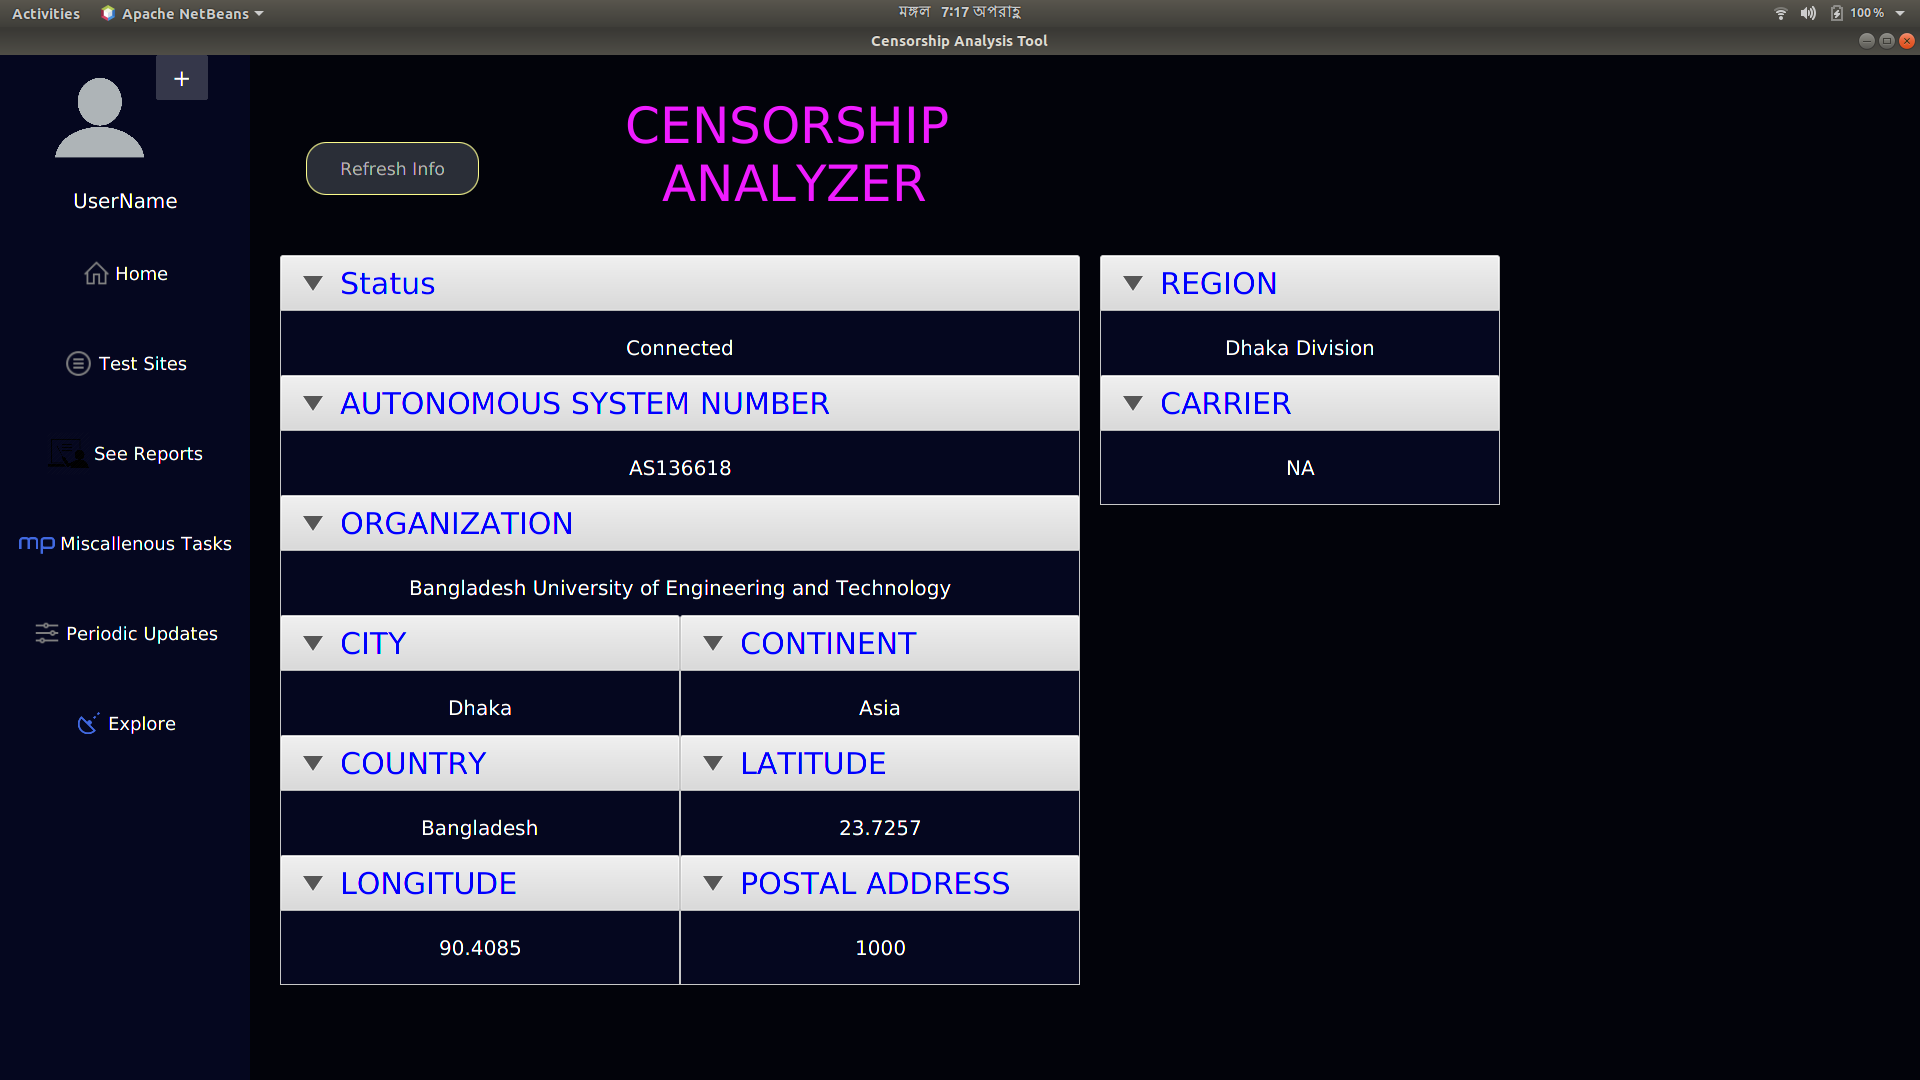
\includegraphics[width=\textwidth]{usersite/home.png}
    \caption{Home page at desktop app}
    \label{fig:user0}
\end{figure}

A user can see his previous reports by clicking \emph{See Reports} button of home page.
He will see all the reports . He can apply various filter on it and after clicking \emph{Refresh} button, he will see filtered test.

\begin{figure}[h]
    \centering
    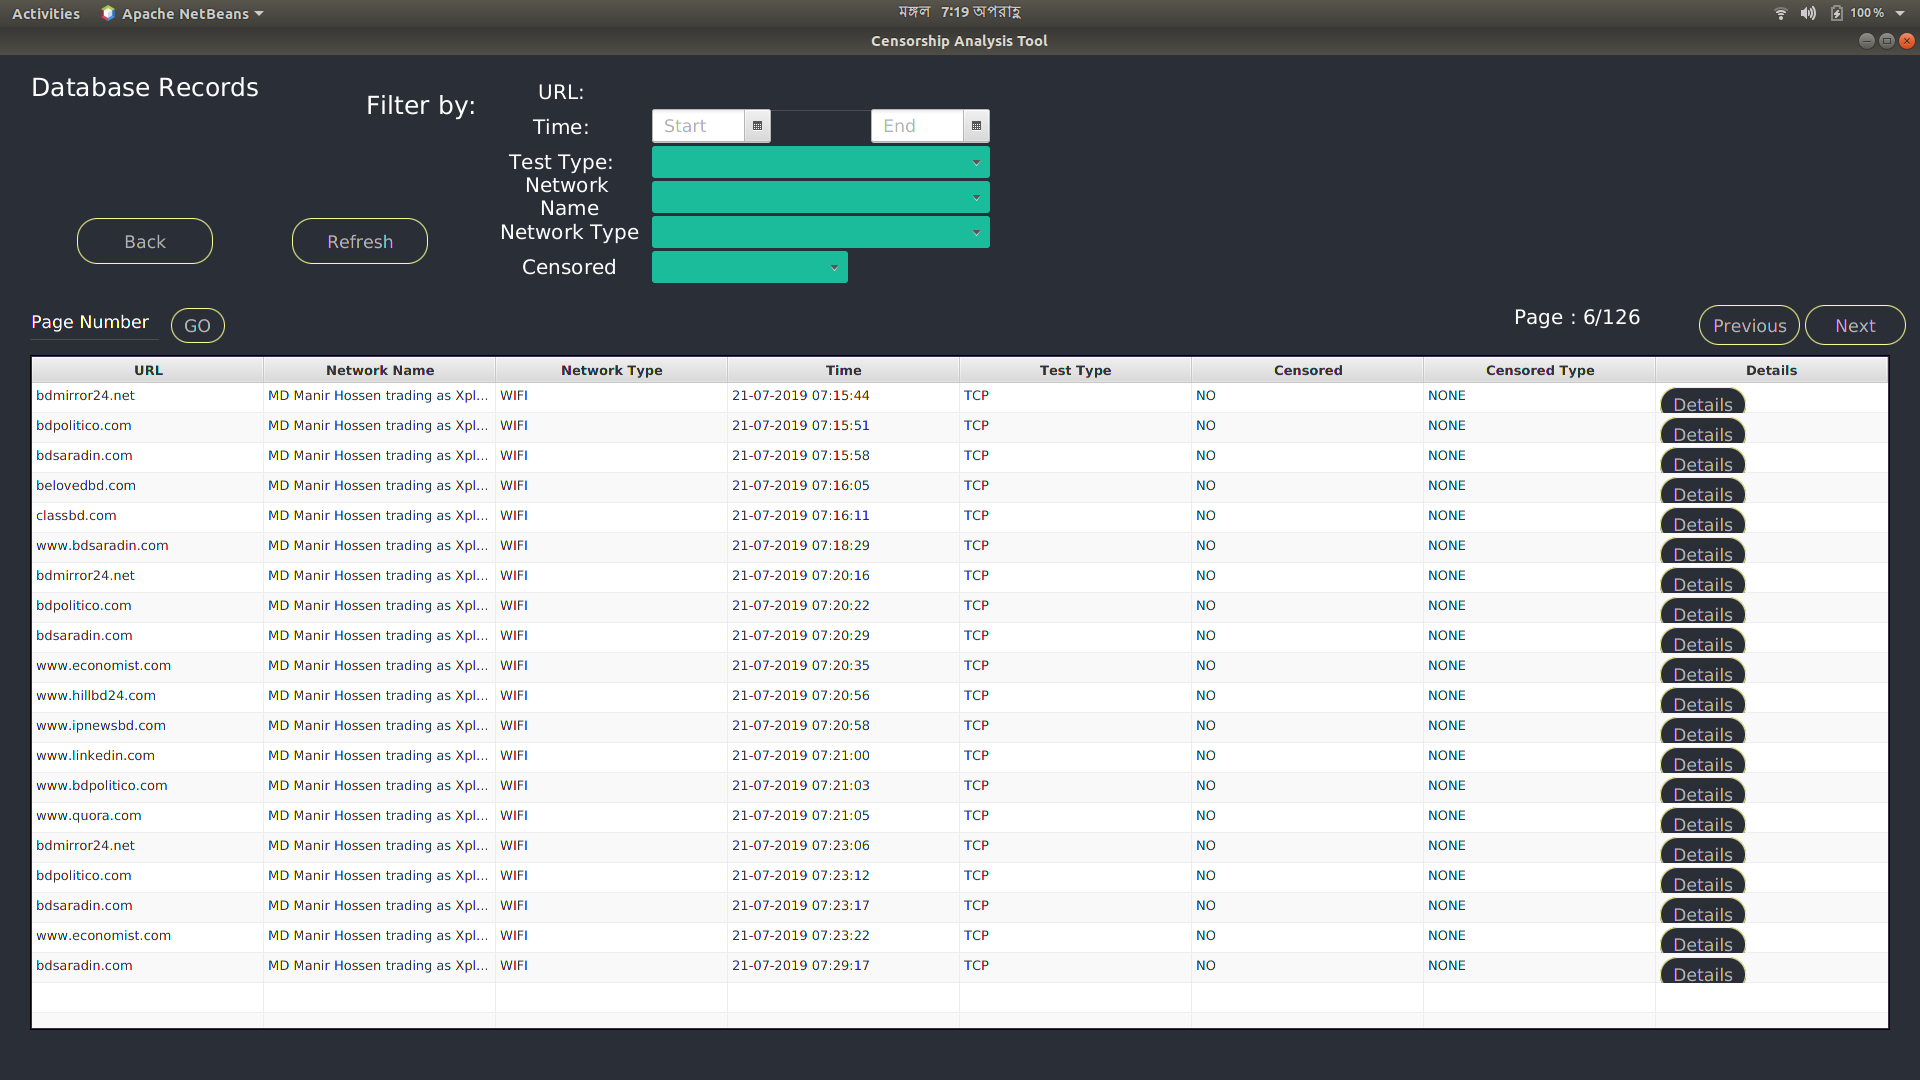
\includegraphics[width=\textwidth]{usersite/1recordswithoutfilter.png}
    \caption{Records without filtering}
    \label{fig:user1}
\end{figure}

\begin{figure}[h]
    \centering
    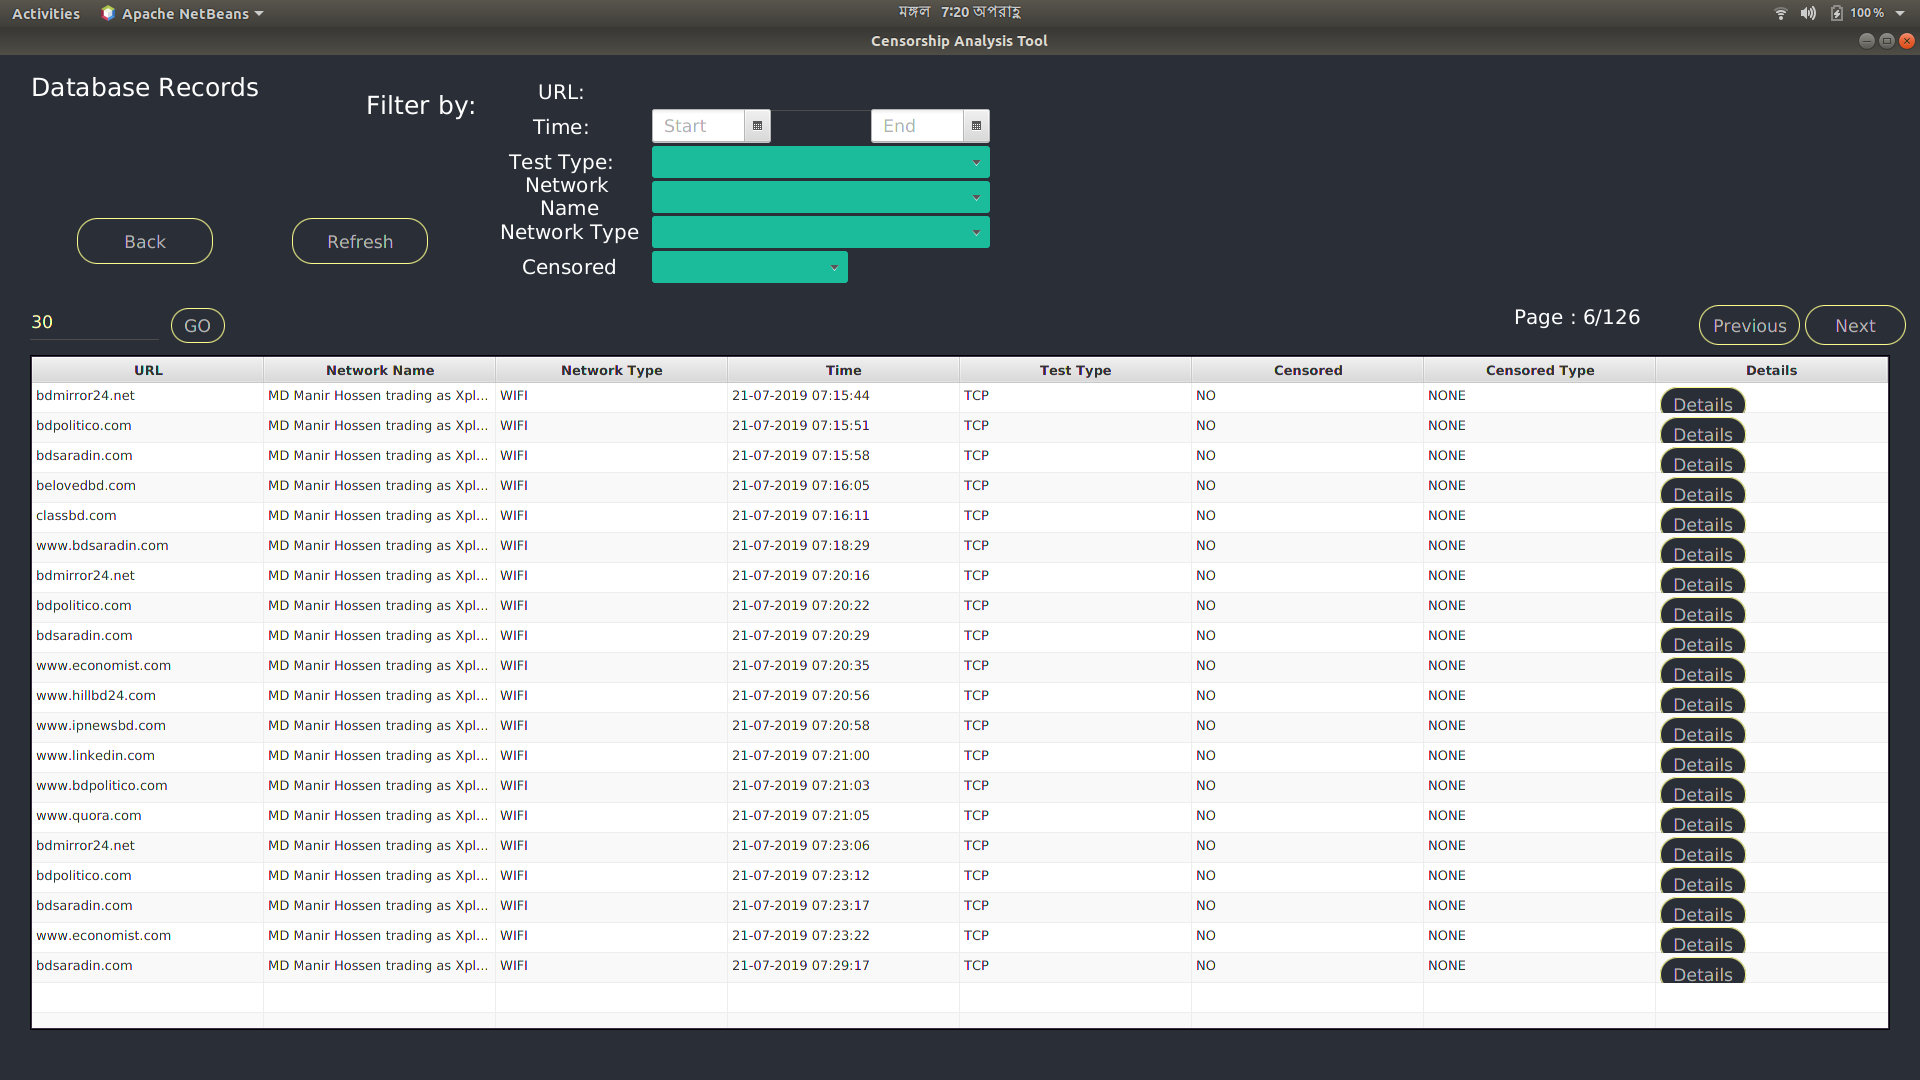
\includegraphics[width=\textwidth]{usersite/2pageinput.png}
    \caption{Inserting page 30}
    \label{fig:user2}
\end{figure}

\begin{figure}[h]
    \centering
    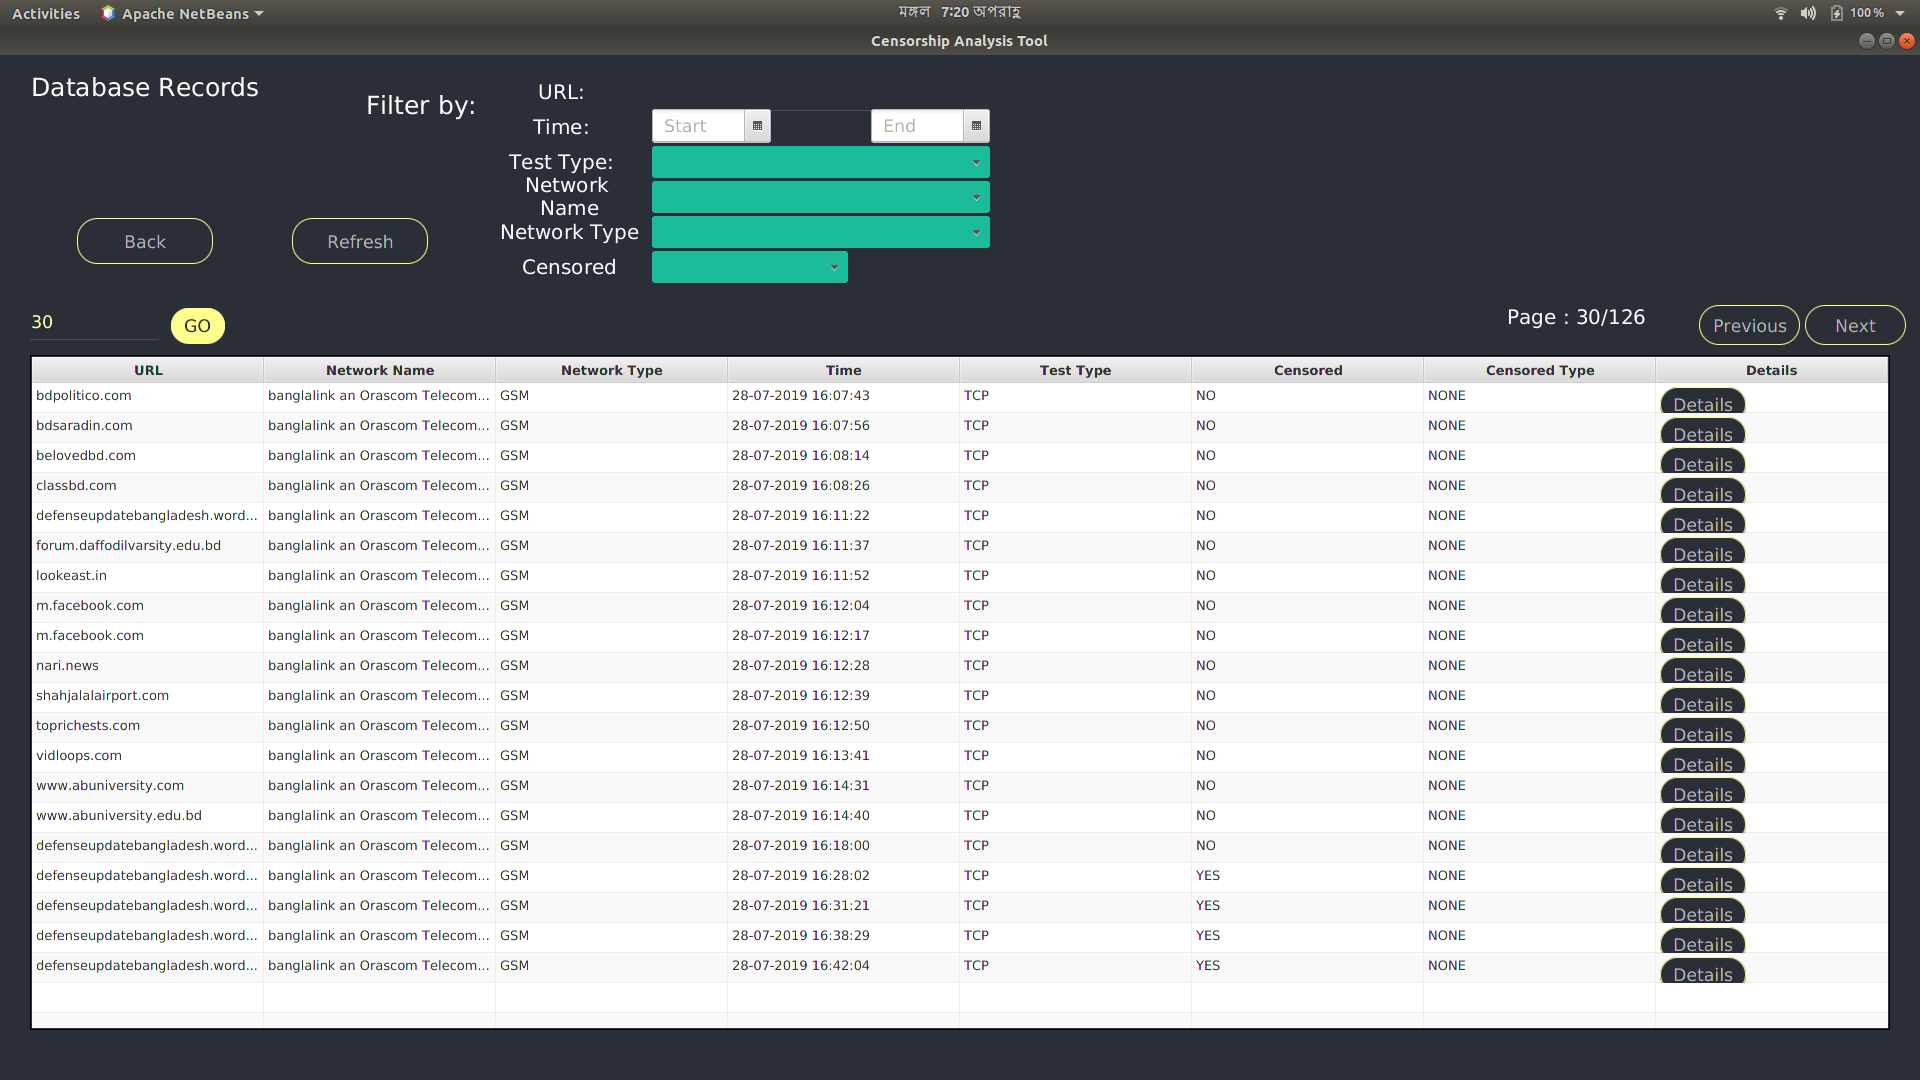
\includegraphics[width=\textwidth]{usersite/3pageoutput.png}
    \caption{At page 30}
    \label{fig:user3}
\end{figure}

\begin{figure}[h]
    \centering
    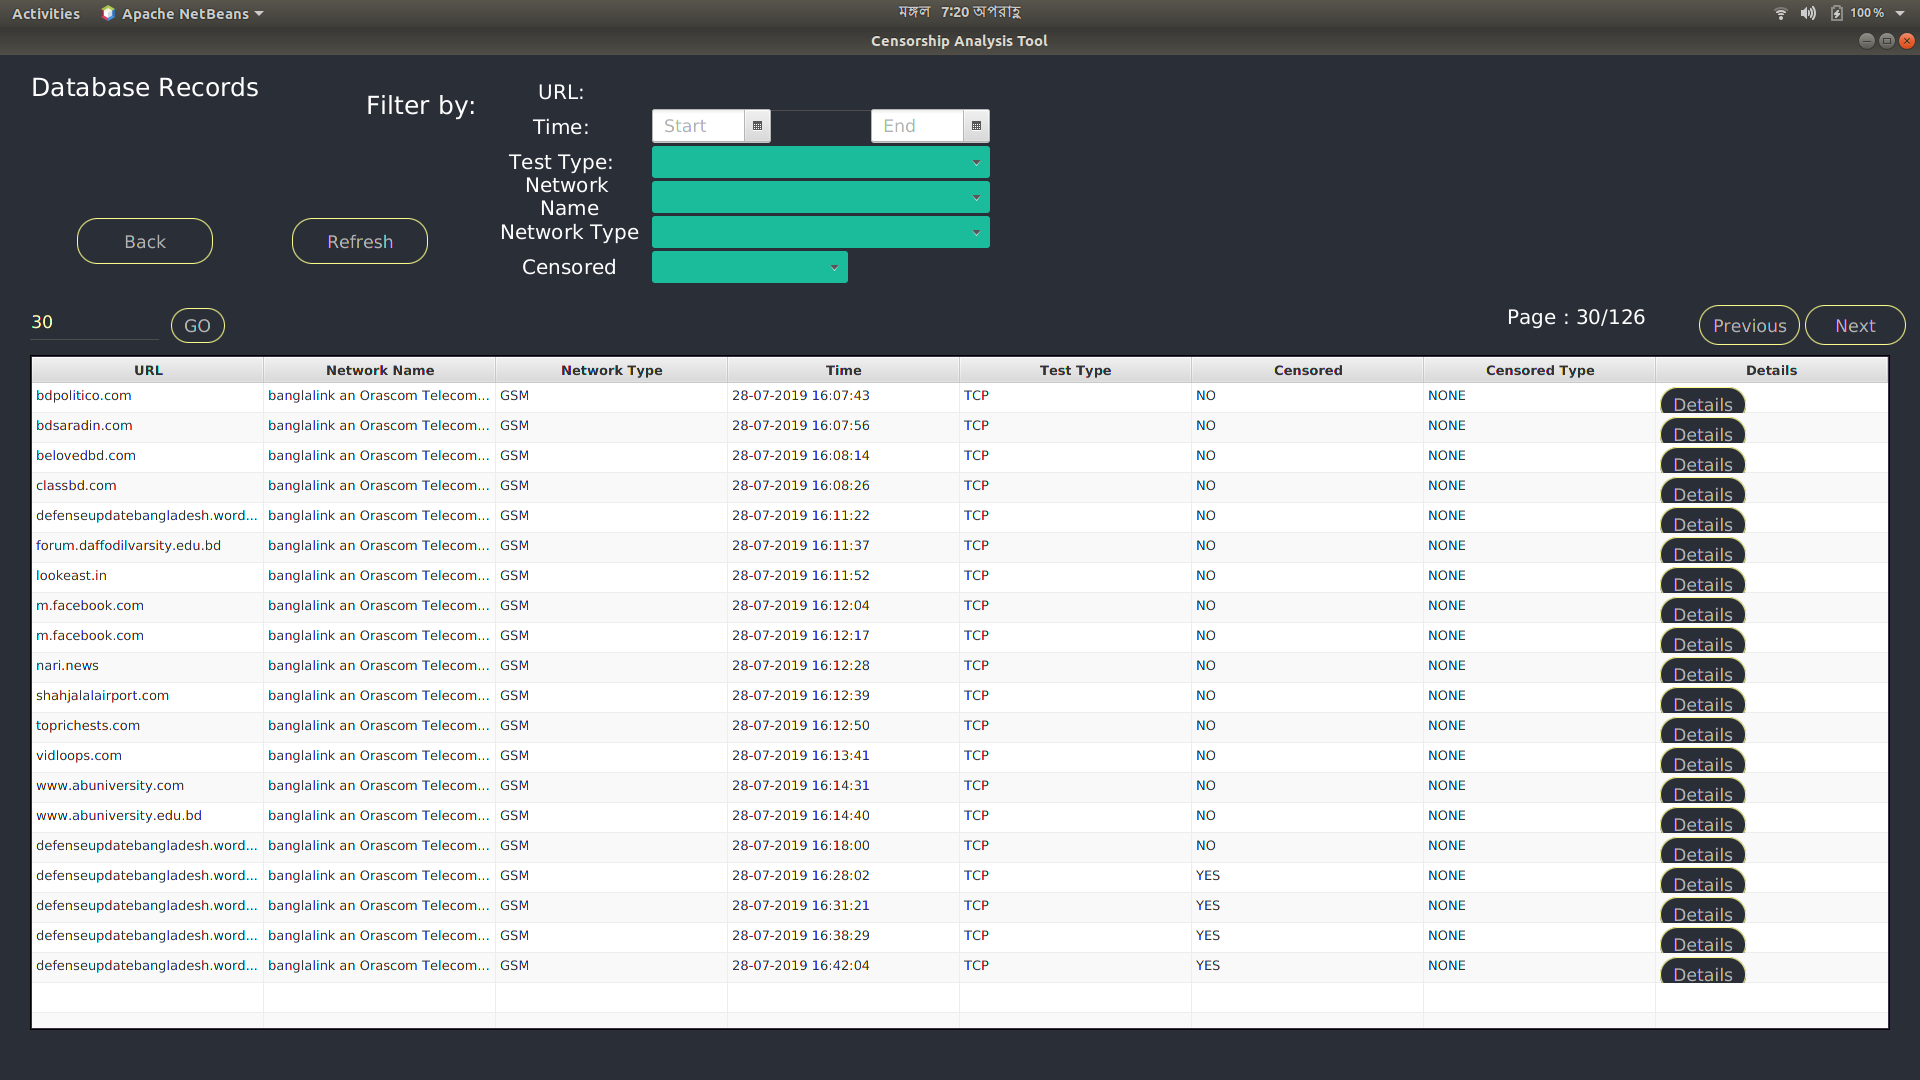
\includegraphics[width=\textwidth]{usersite/4withoutfilter.png}
    \caption{Agin test are without filter}
    \label{fig:user4}
\end{figure}

\begin{figure}[h]
    \centering
    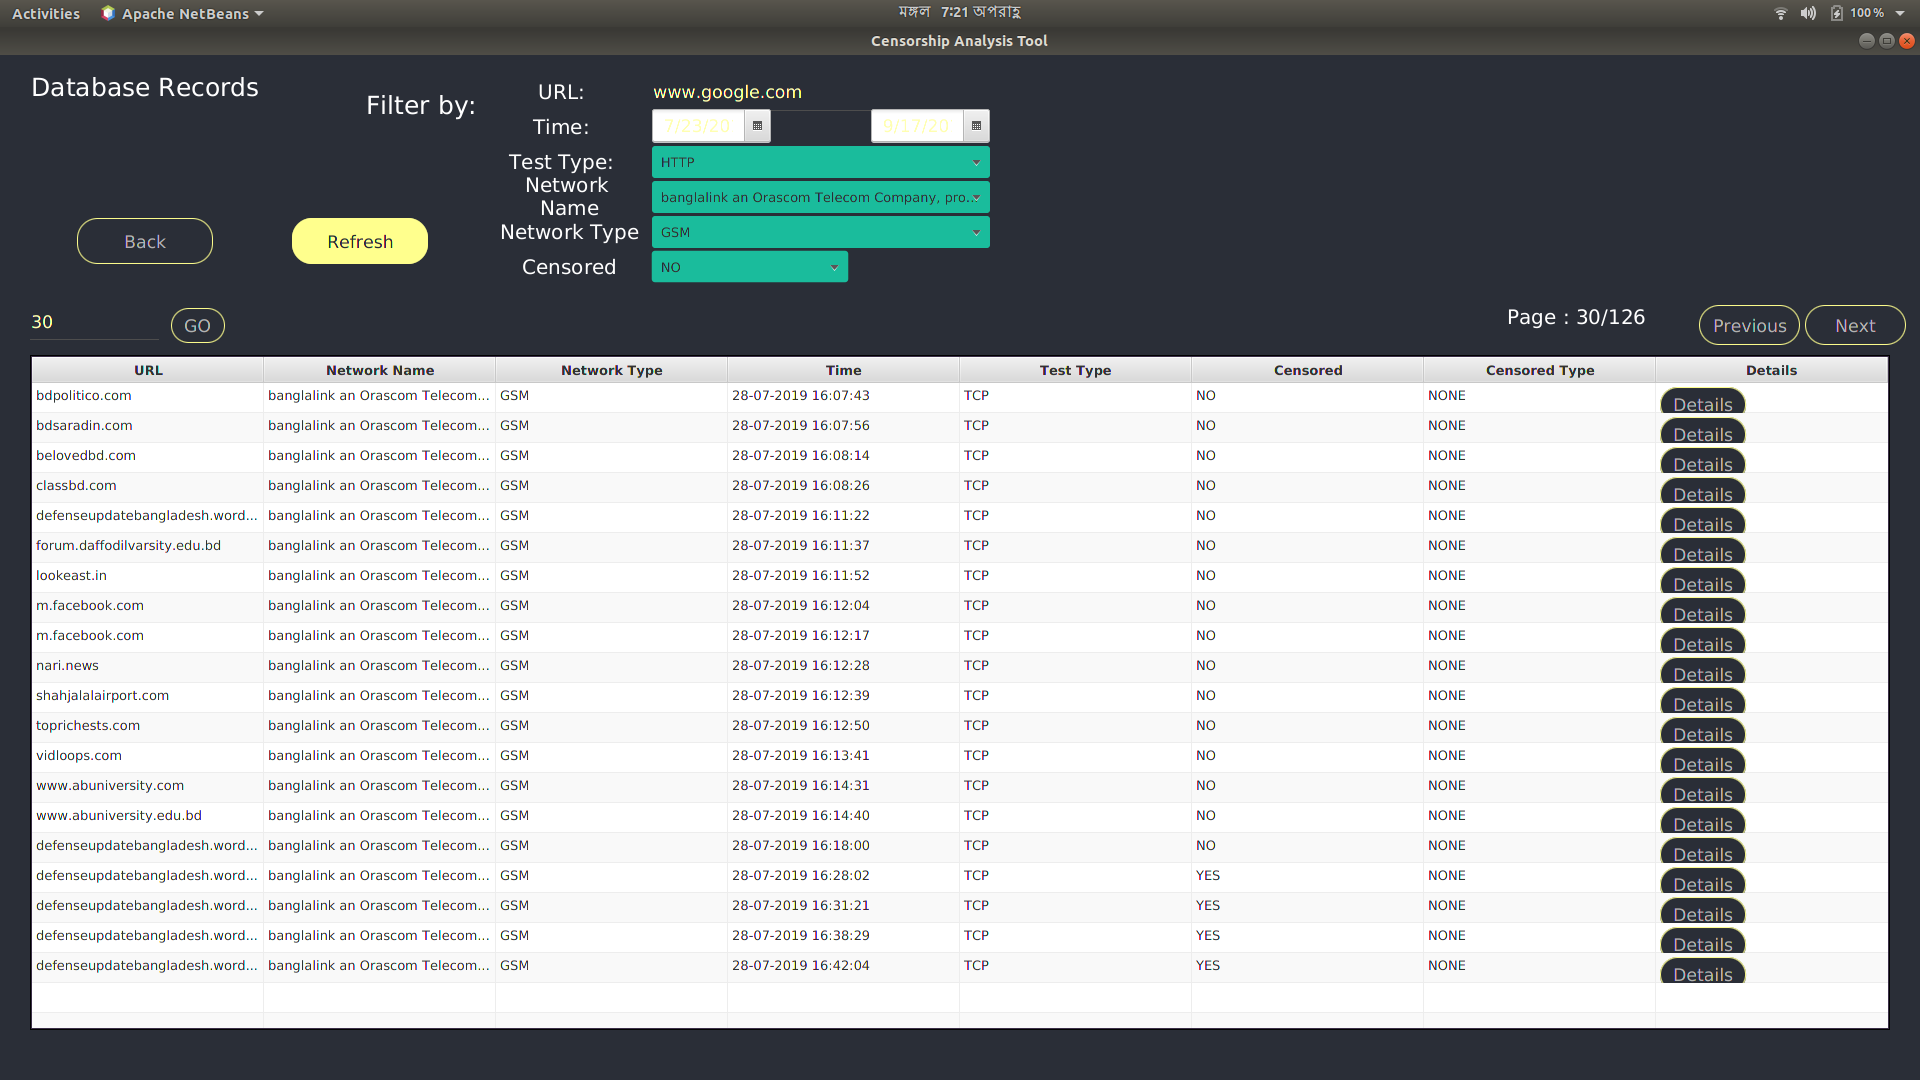
\includegraphics[width=\textwidth]{usersite/5beforefilter.png}
    \caption{Before applying filter}
    \label{fig:user5}
\end{figure}

\begin{figure}[h]
    \centering
    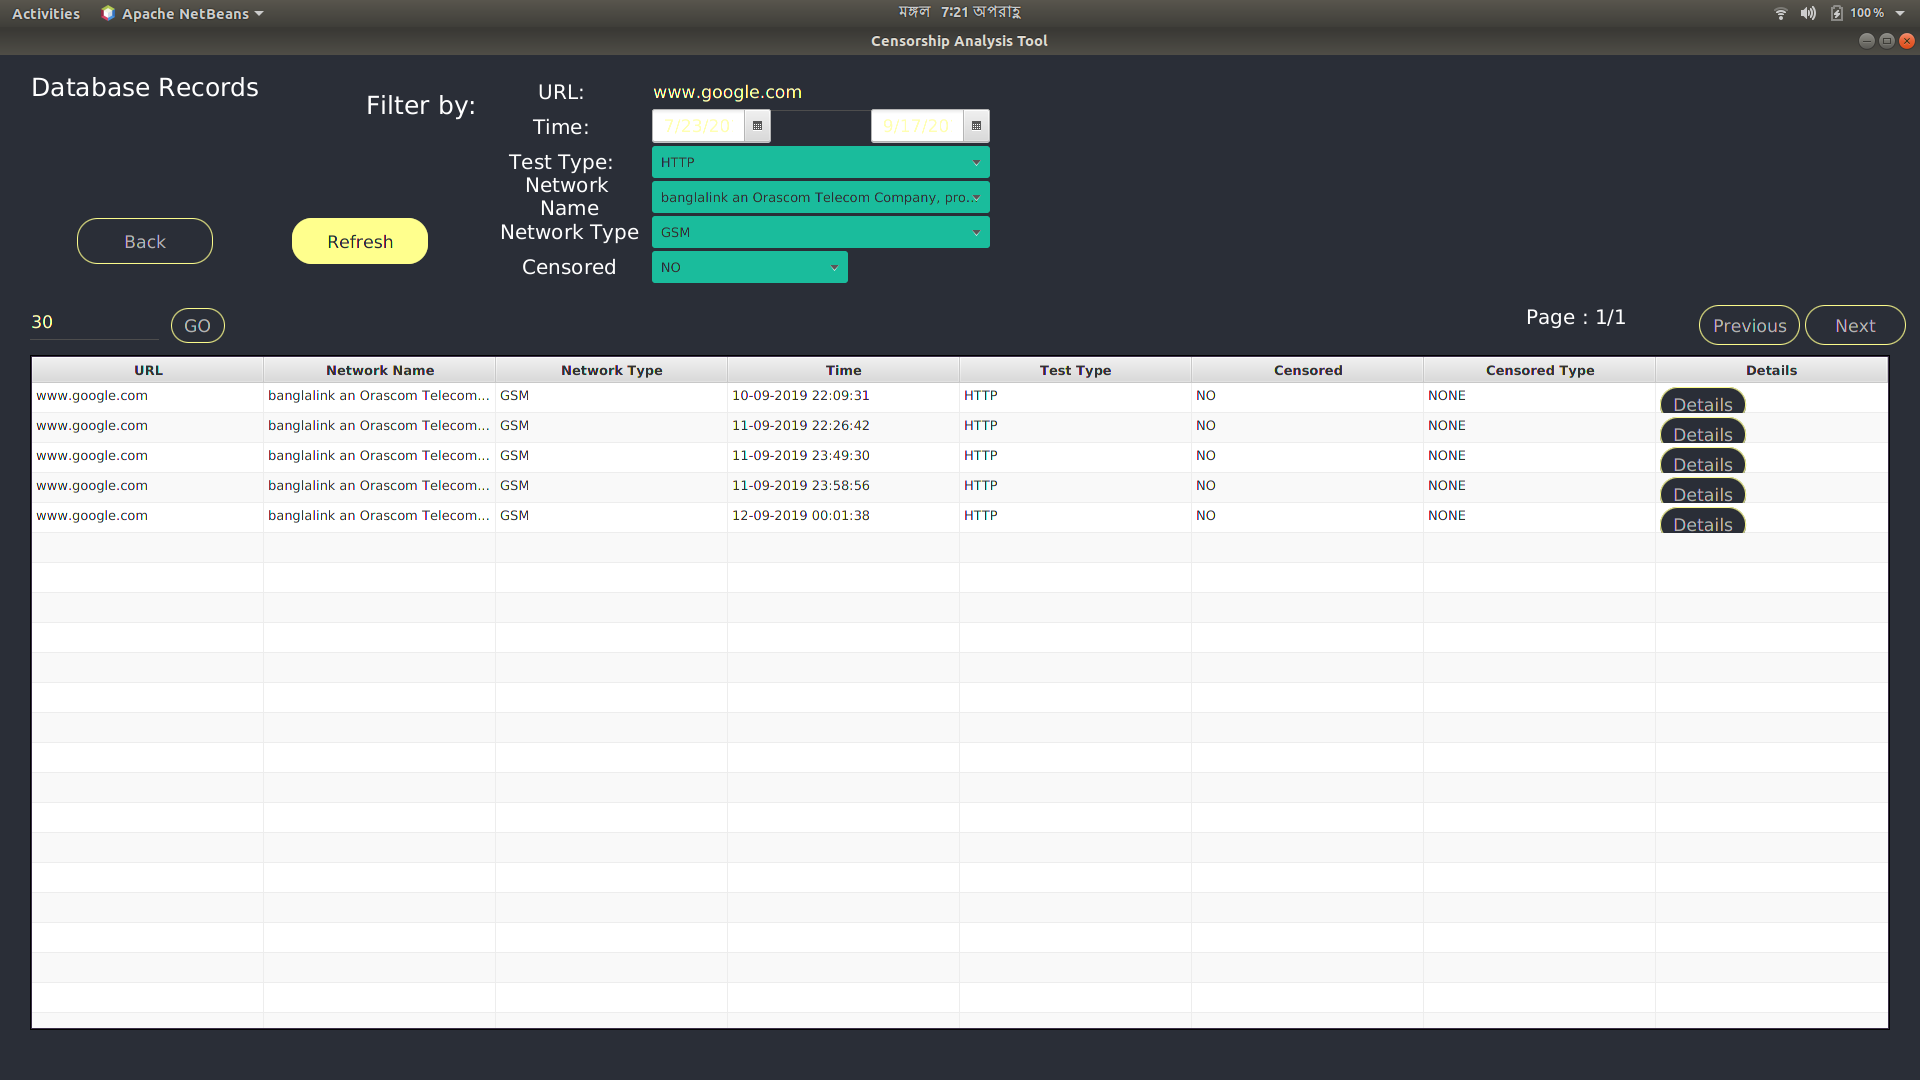
\includegraphics[width=\textwidth]{usersite/6afterfilter.png}
    \caption{After applying various filter}
    \label{fig:user6}
\end{figure}

After clicking \emph{Back} button, a user can come to home page again. 
\begin{figure}[h]
    \centering
    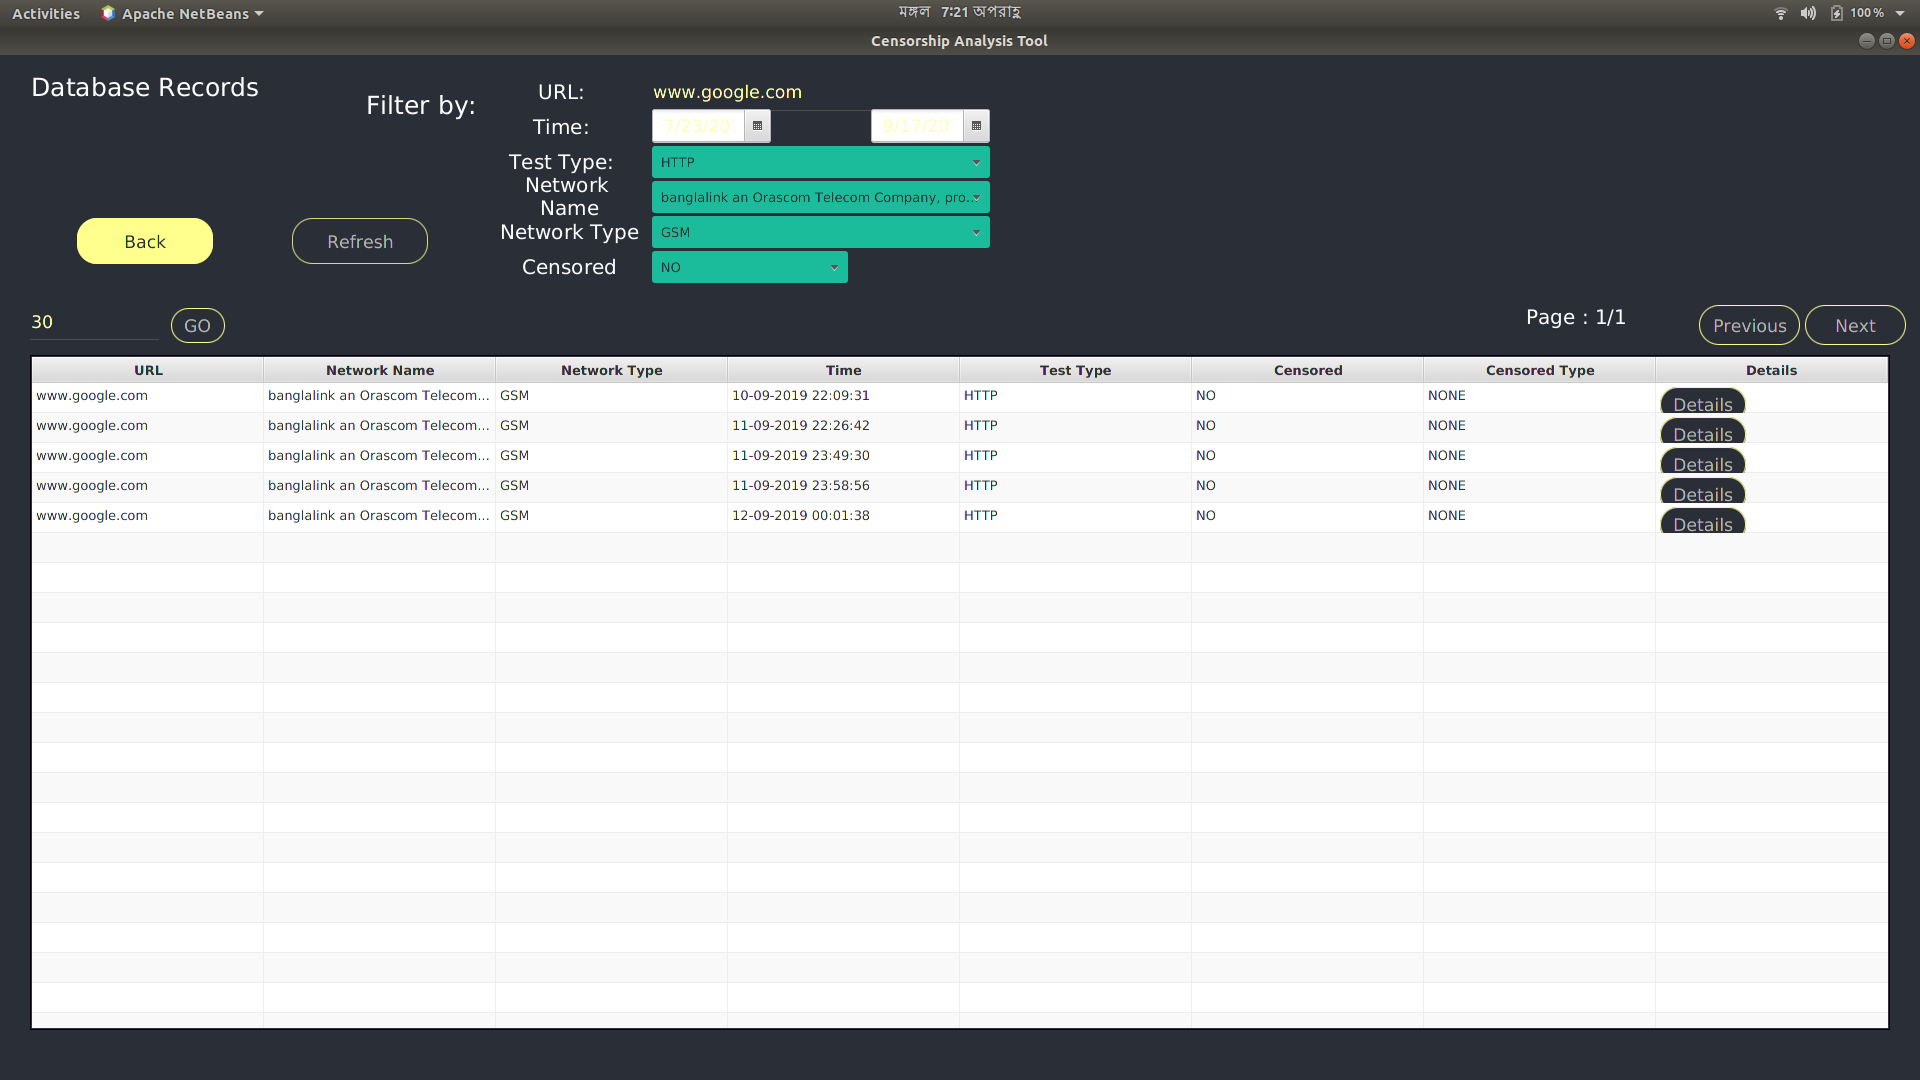
\includegraphics[width=\textwidth]{usersite/7back.png}
    \caption{Clicking back button}
    \label{fig:user7}
\end{figure}

\begin{figure}[h]
    \centering
    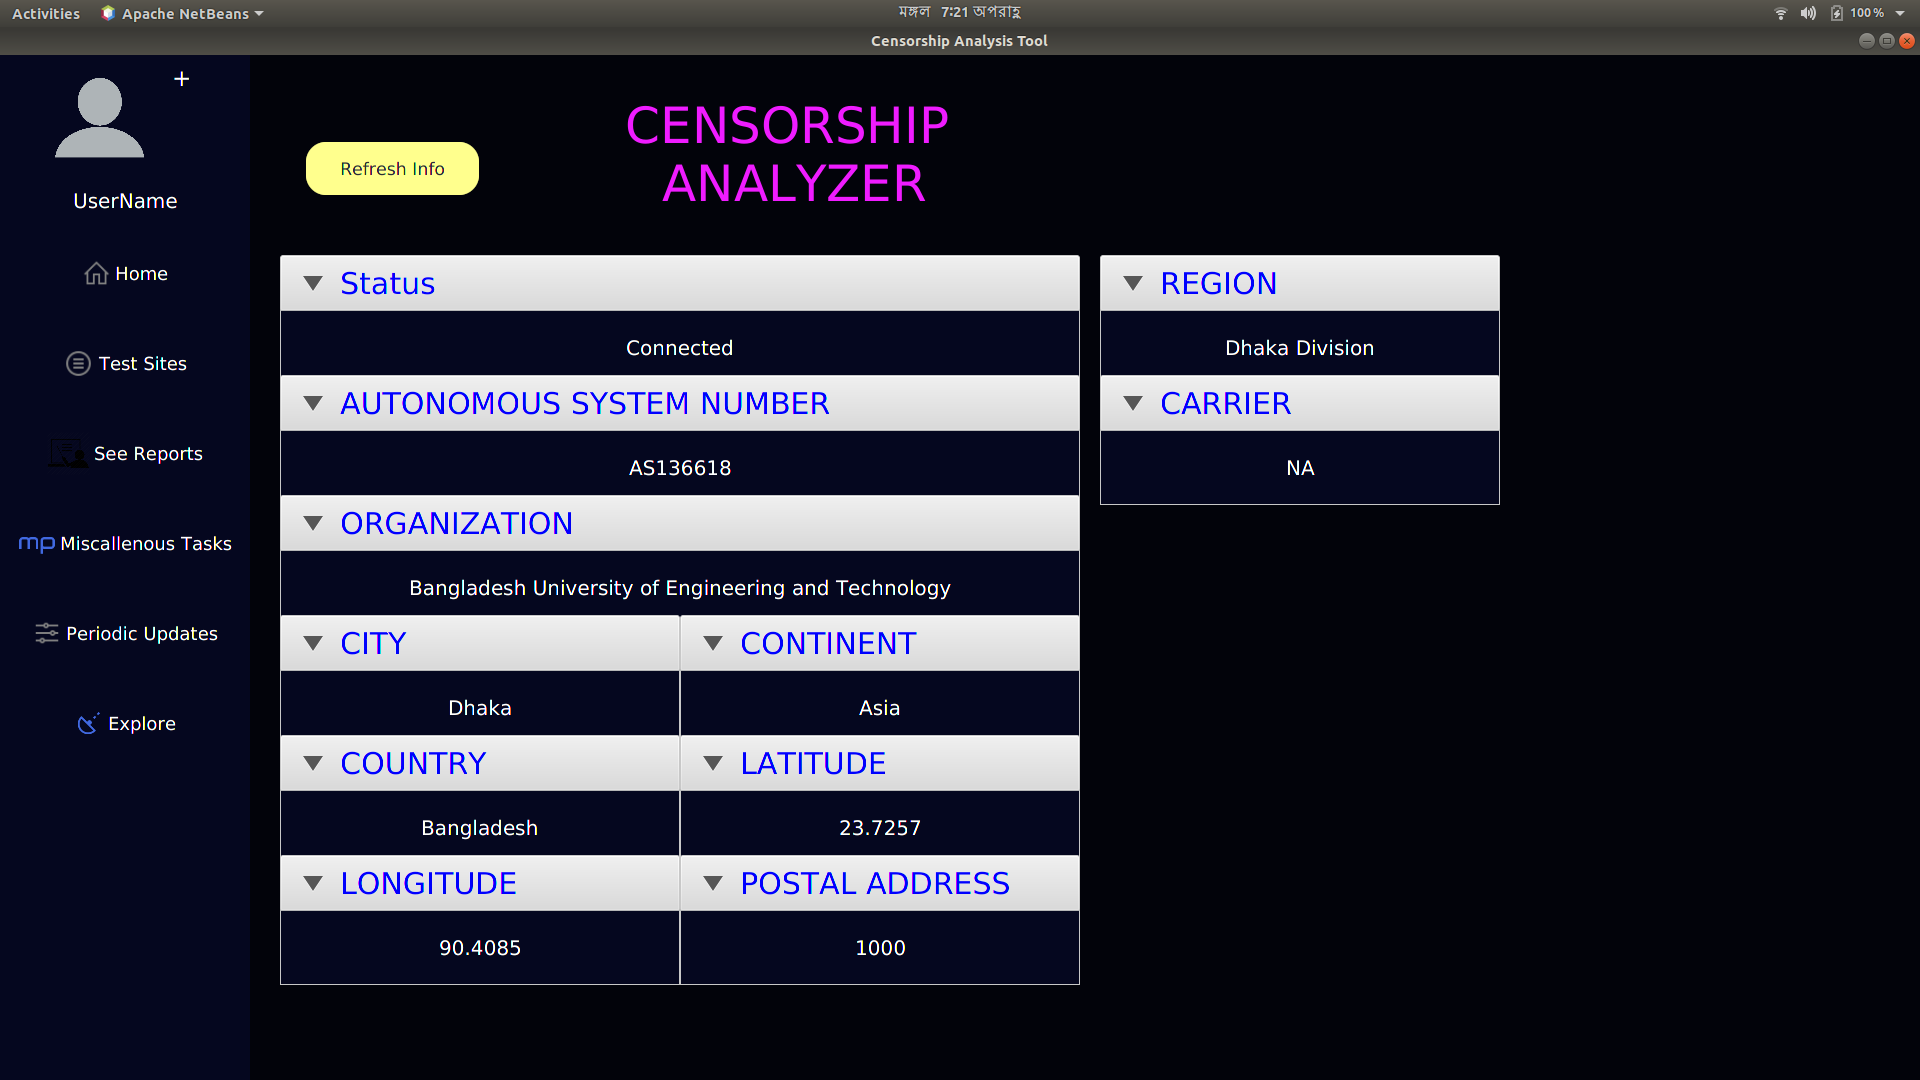
\includegraphics[width=\textwidth]{usersite/8homepage.png}
    \caption{Home page back}
    \label{fig:user8}
\end{figure}

After clicking \emph{Test Sites} a user should test single url or files of url by clicking file selector, selecting type of test and accepting all terms and condition submit the test query. He can see file's data by clicking \emph{View File} button.
\begin{figure}[h]
    \centering
    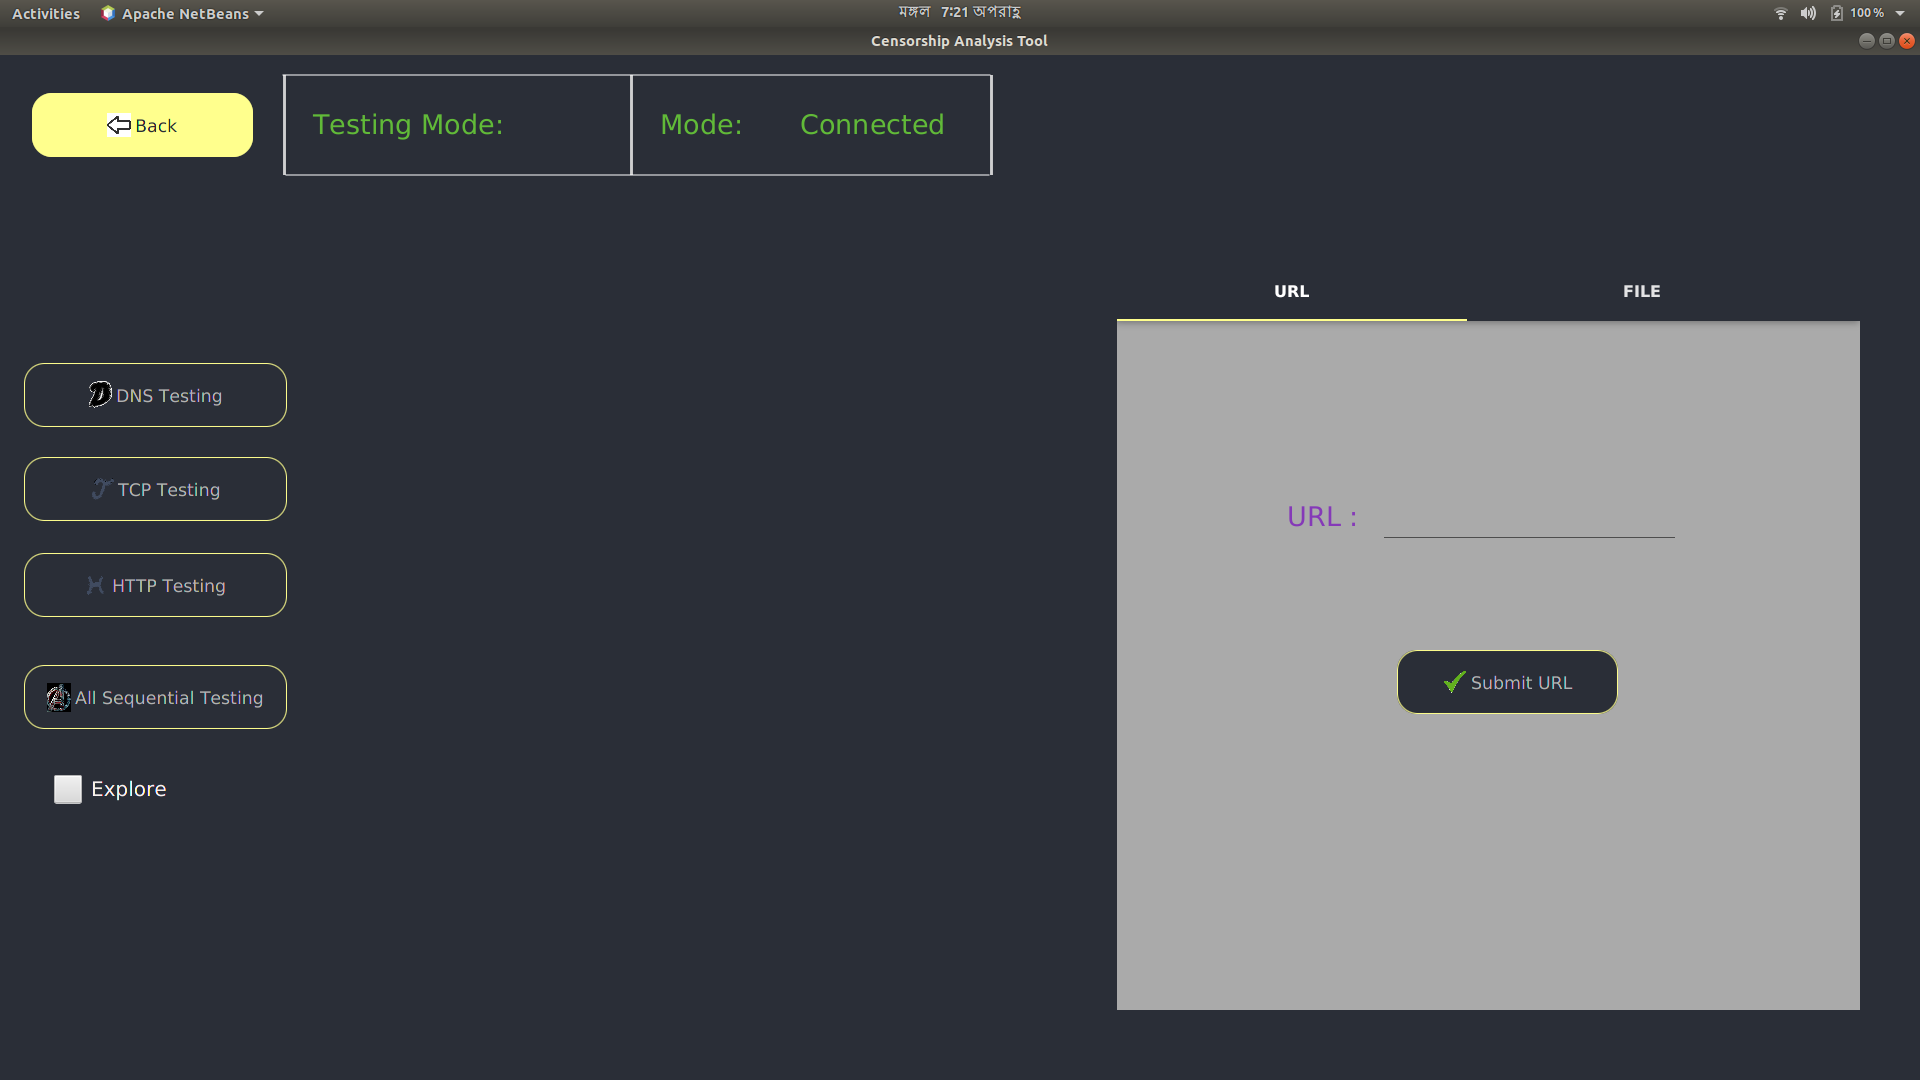
\includegraphics[width=\textwidth]{usersite/9dnstest.png}
    \caption{A sample testing window}
    \label{fig:user9}
\end{figure}

\begin{figure}[h]
    \centering
    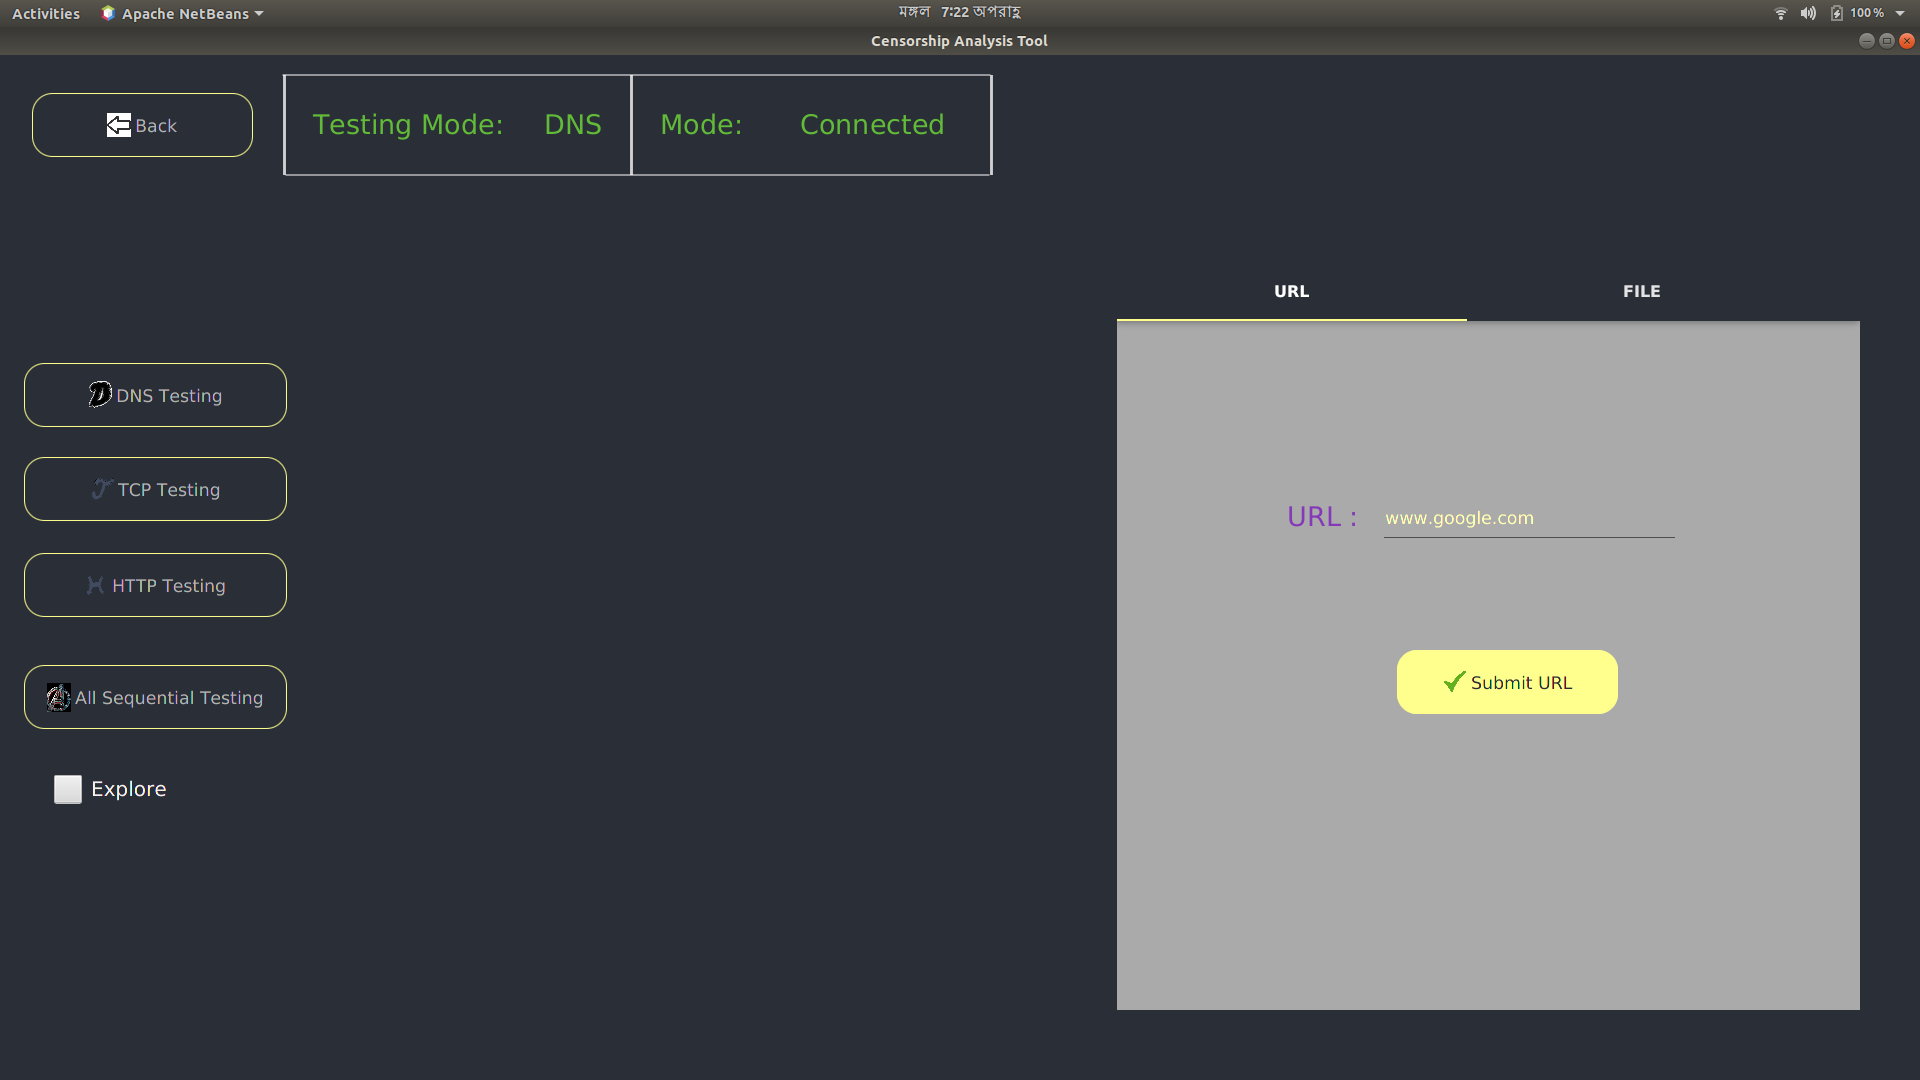
\includegraphics[width=\textwidth]{usersite/10input.png}
    \caption{Another dns test input}
    \label{fig:user10}
\end{figure}


\begin{figure}[h]
    \centering
    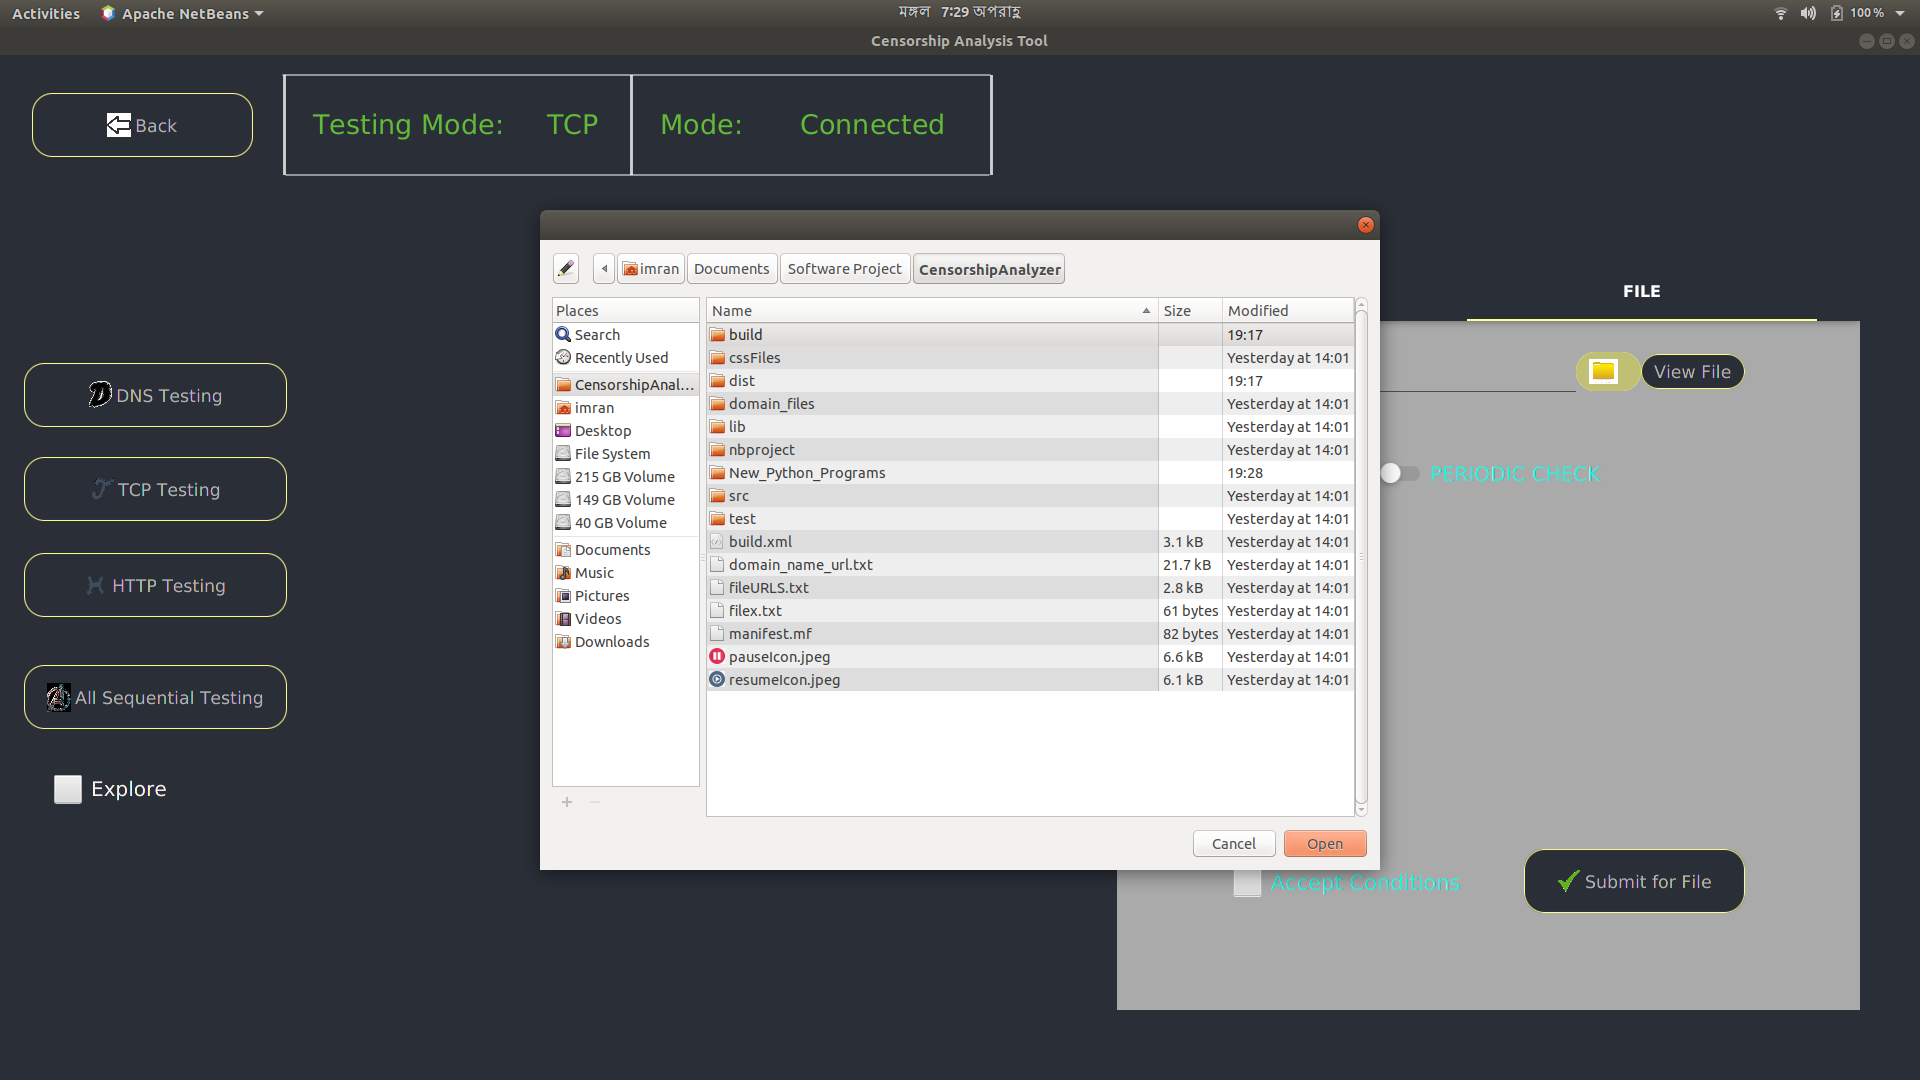
\includegraphics[width=\textwidth]{usersite/26selectfiles.png}
    \caption{File with urls can be selected to test}
    \label{fig:user25}
\end{figure}


\begin{figure}[h]
    \centering
    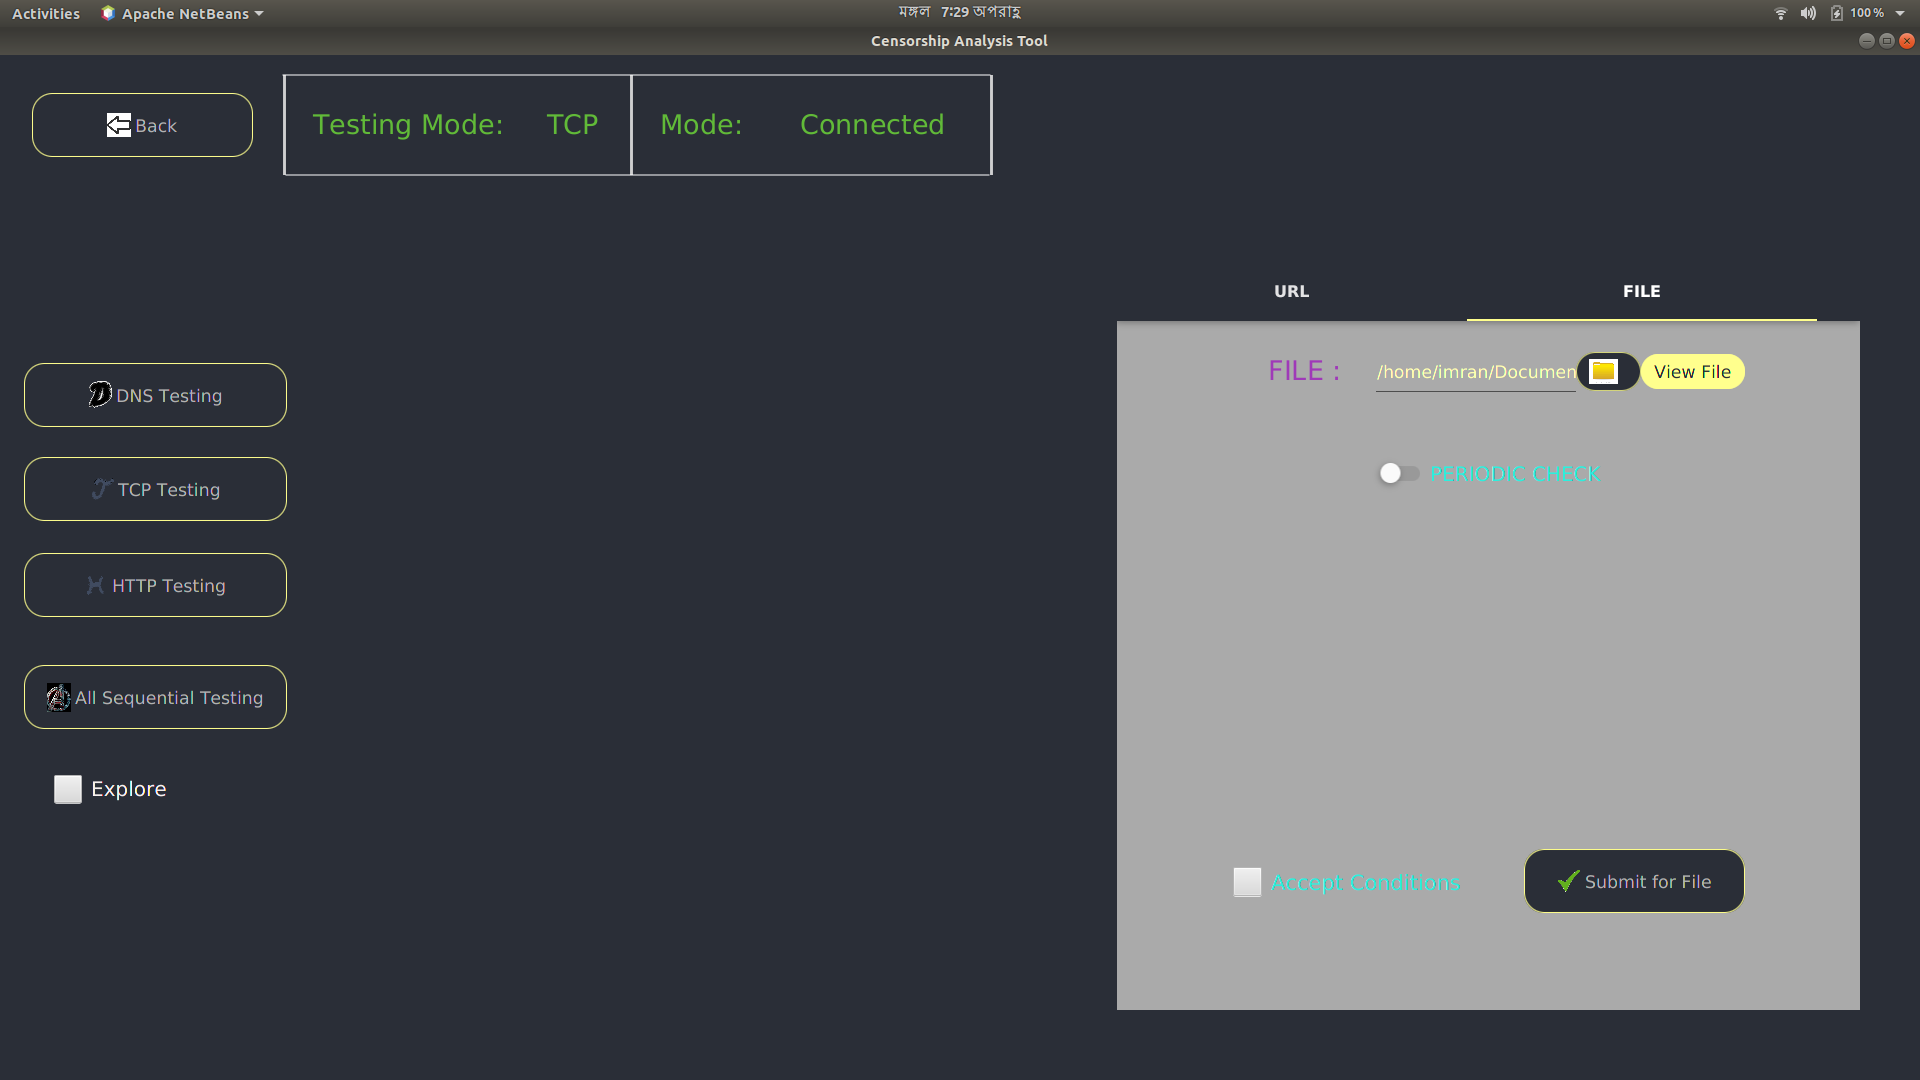
\includegraphics[width=\textwidth]{usersite/27inputfile2.png}
    \caption{Selected file url is seen}
    \label{fig:user26}
\end{figure}

\begin{figure}[h]
    \centering
    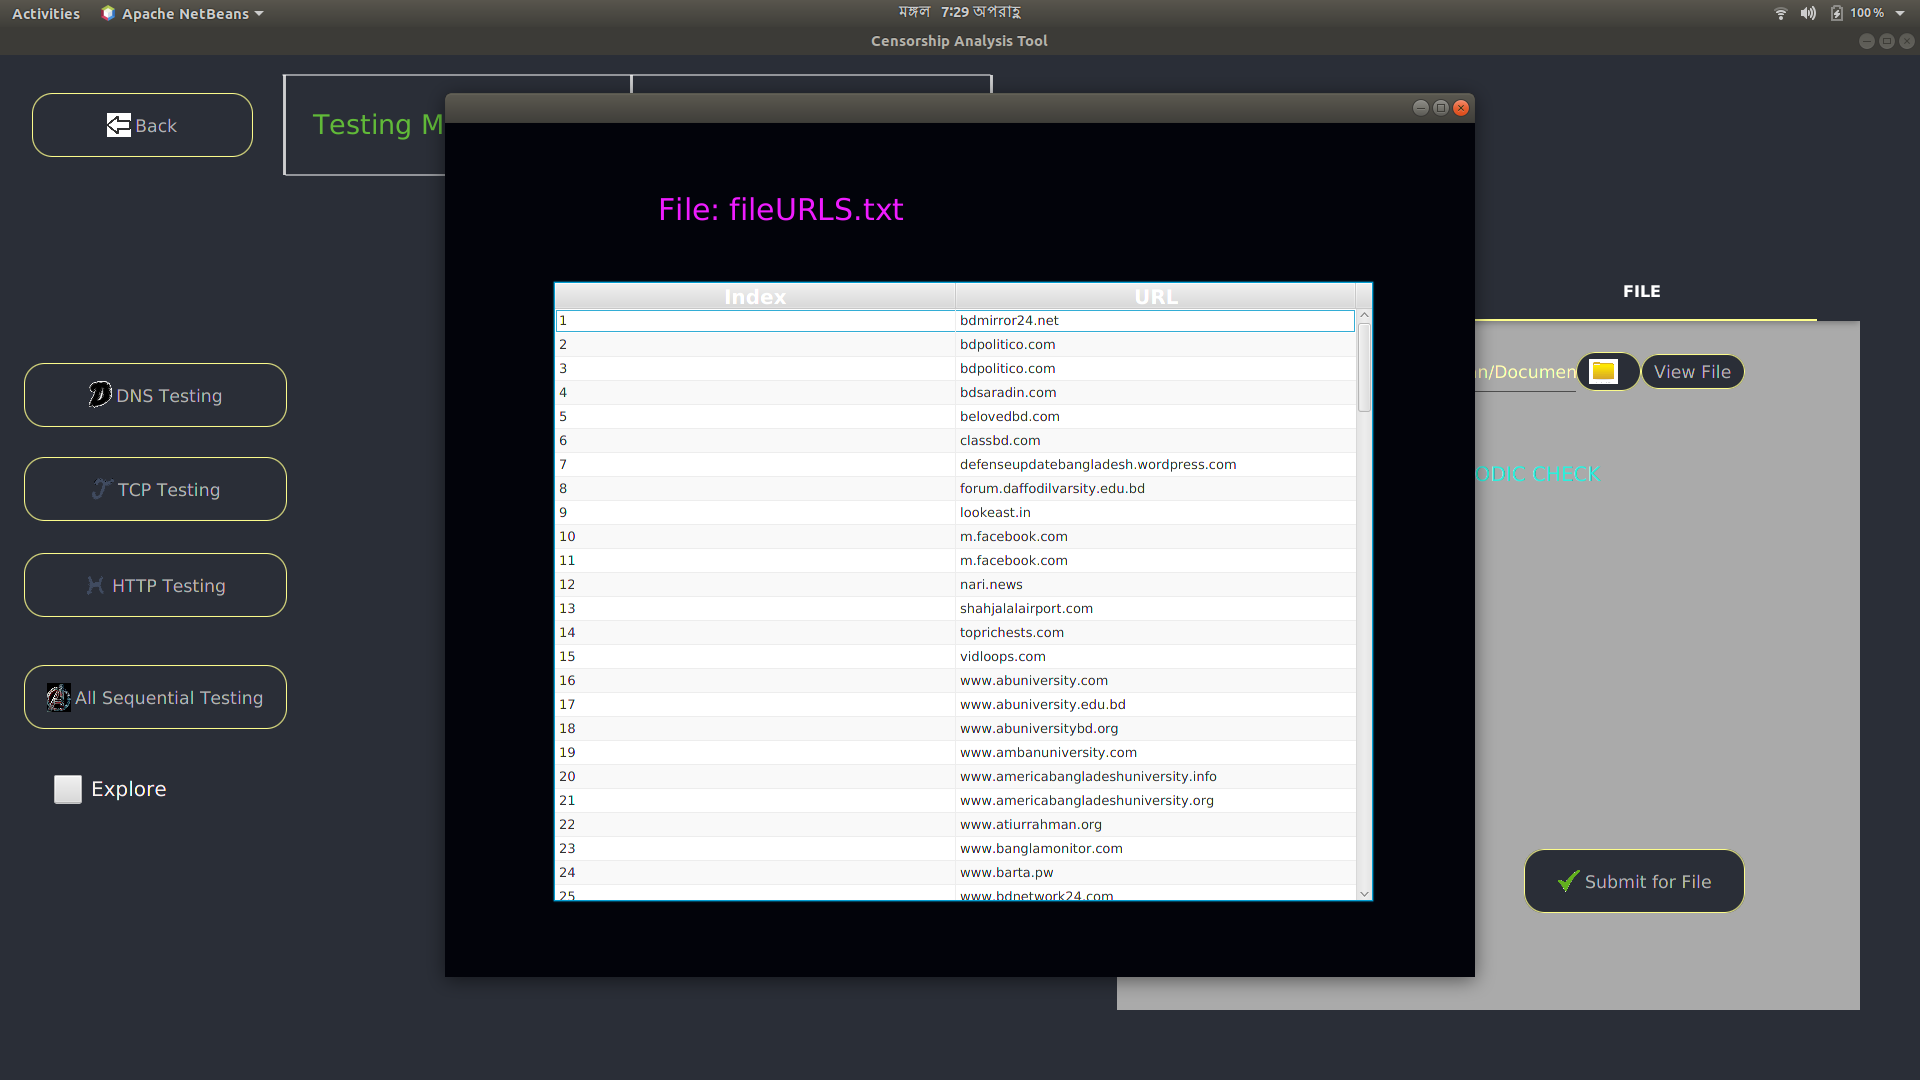
\includegraphics[width=\textwidth]{usersite/28fileread.png}
    \caption{File's url can be seen}
    \label{fig:user27}
\end{figure}



\begin{figure}[h]
    \centering
    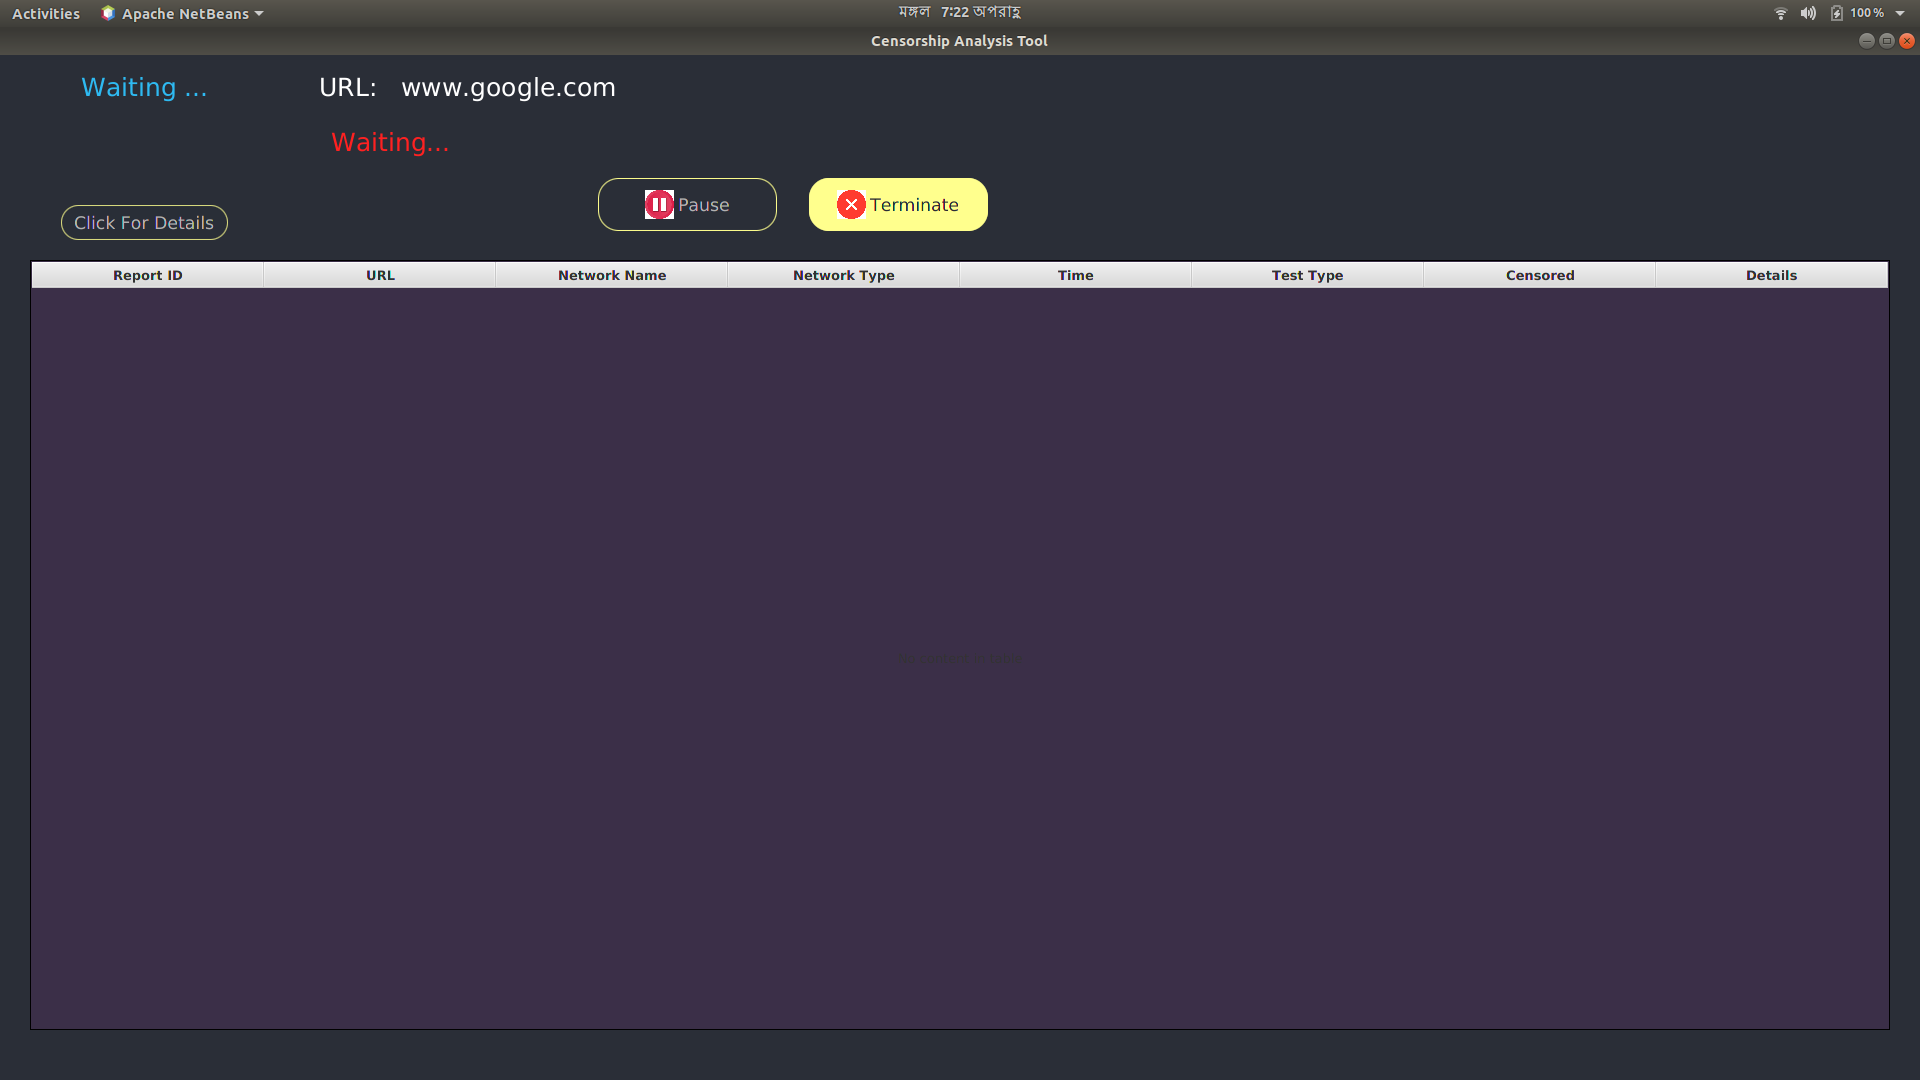
\includegraphics[width=\textwidth]{usersite/11waiting.png}
    \caption{After inserting input of testing new dynamic window appeared}
    \label{fig:user11}
\end{figure}

A user can terminate or pause the testing by clicking \emph{Terminate} and \emph{Pause} button respectively.
\begin{figure}[h]
    \centering
    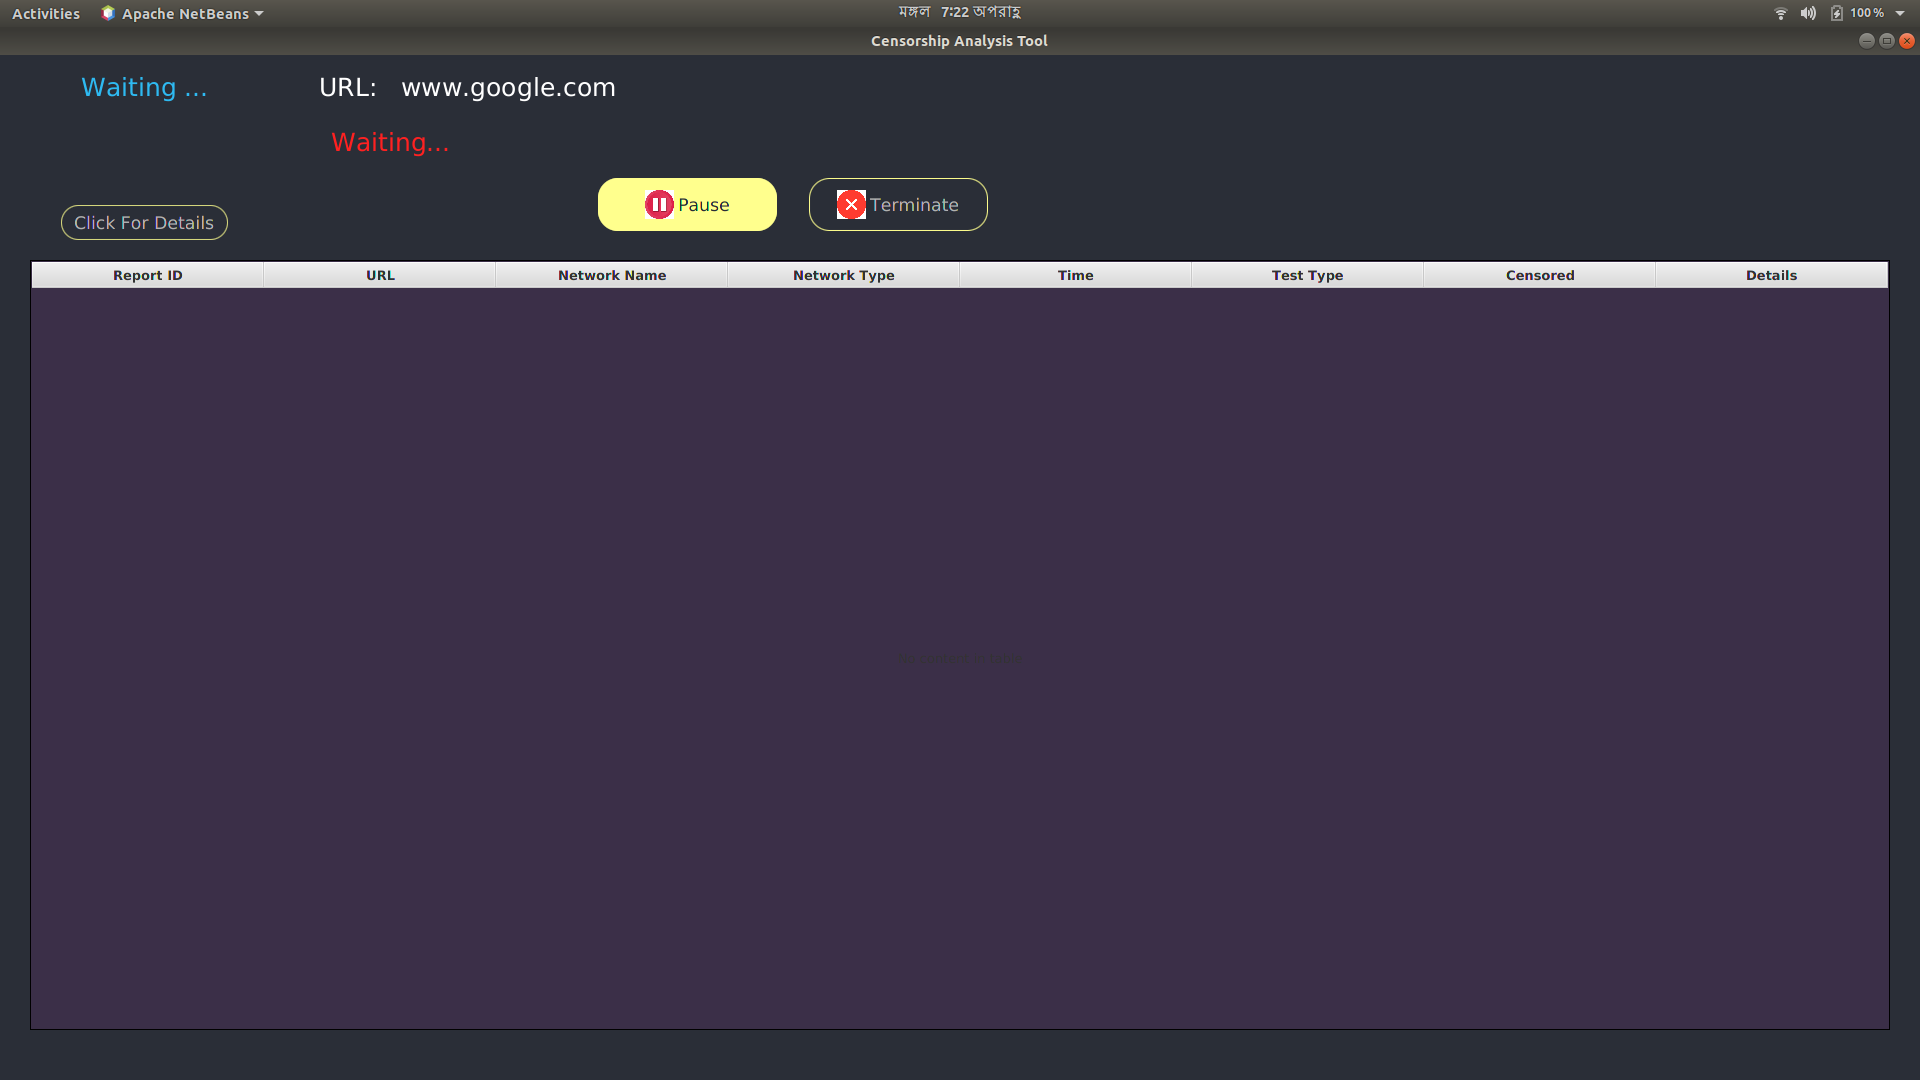
\includegraphics[width=\textwidth]{usersite/12pause.png}
    \caption{After clicking pause button}
    \label{fig:user12}
\end{figure}

\begin{figure}[h]
    \centering
    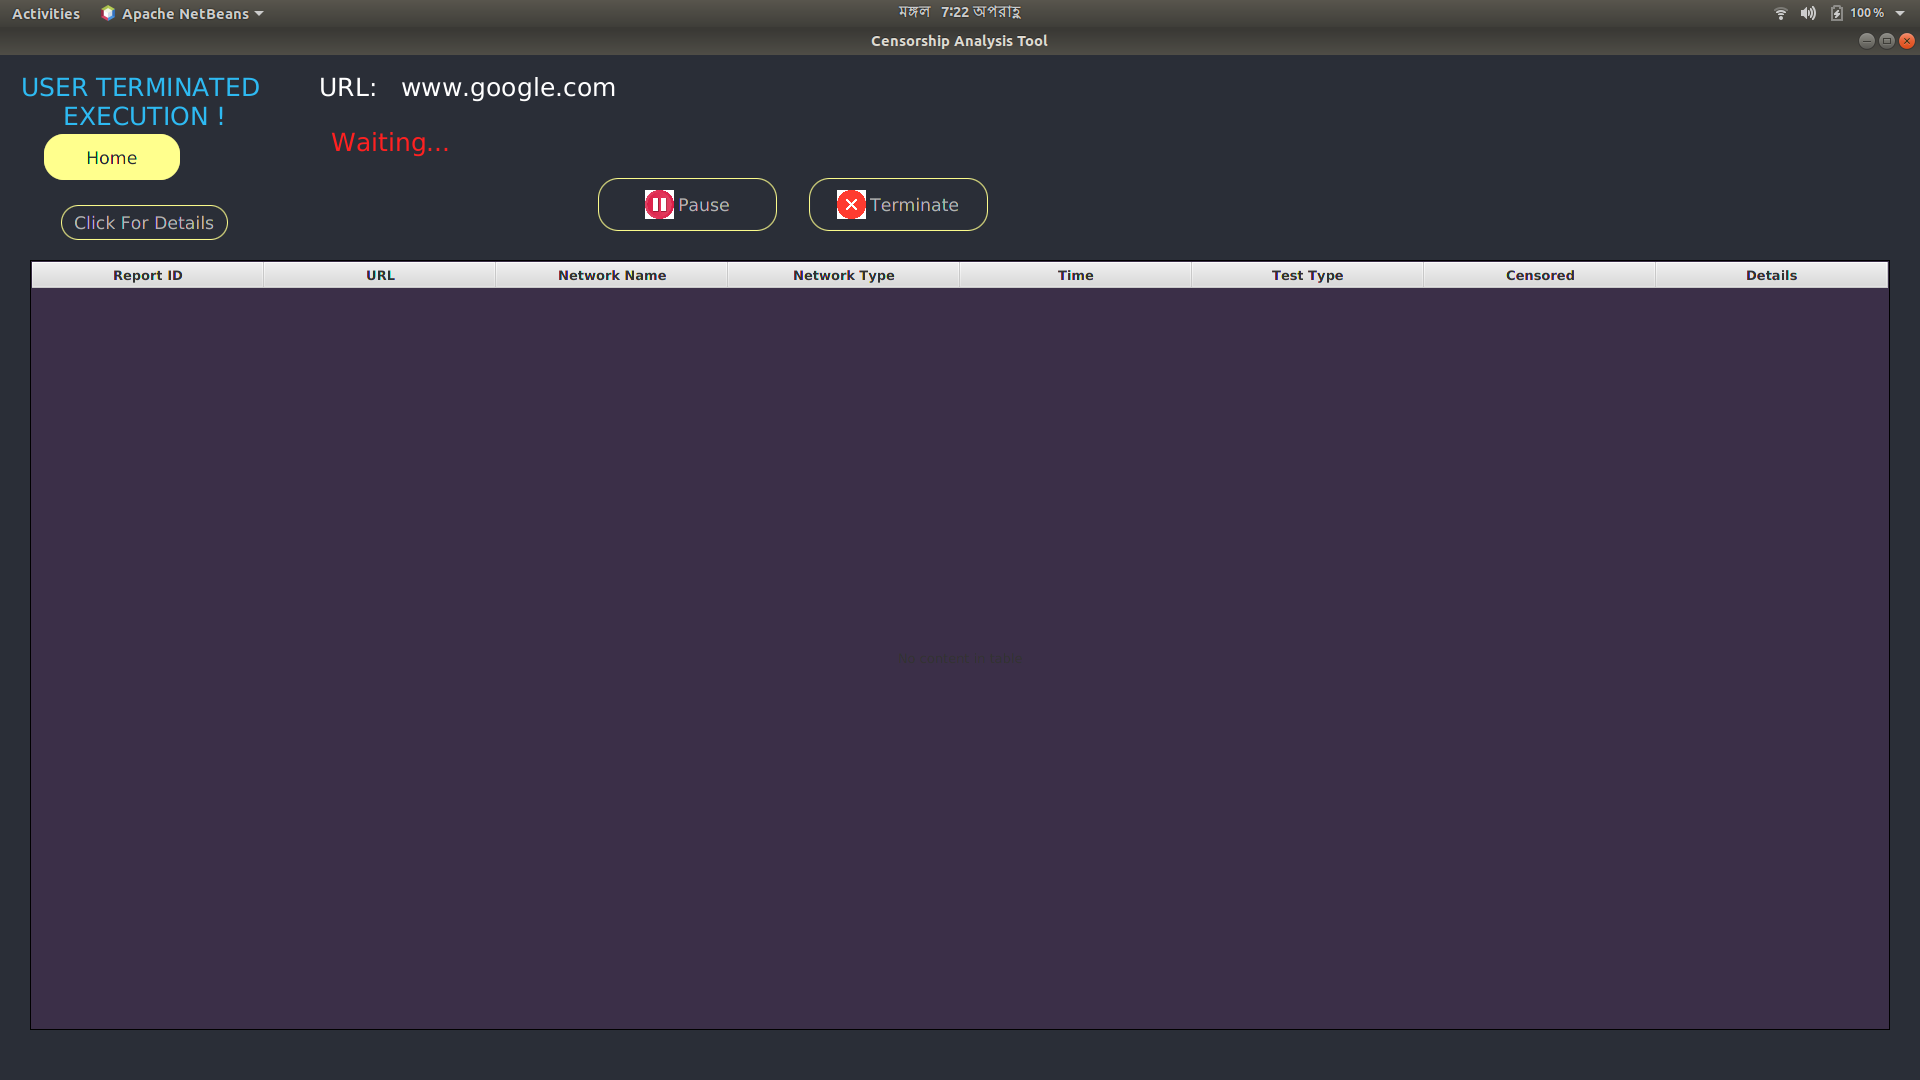
\includegraphics[width=\textwidth]{usersite/13paused.png}
    \caption{After clicking terminate button}
    \label{fig:user13}
\end{figure}

\begin{figure}[h]
    \centering
    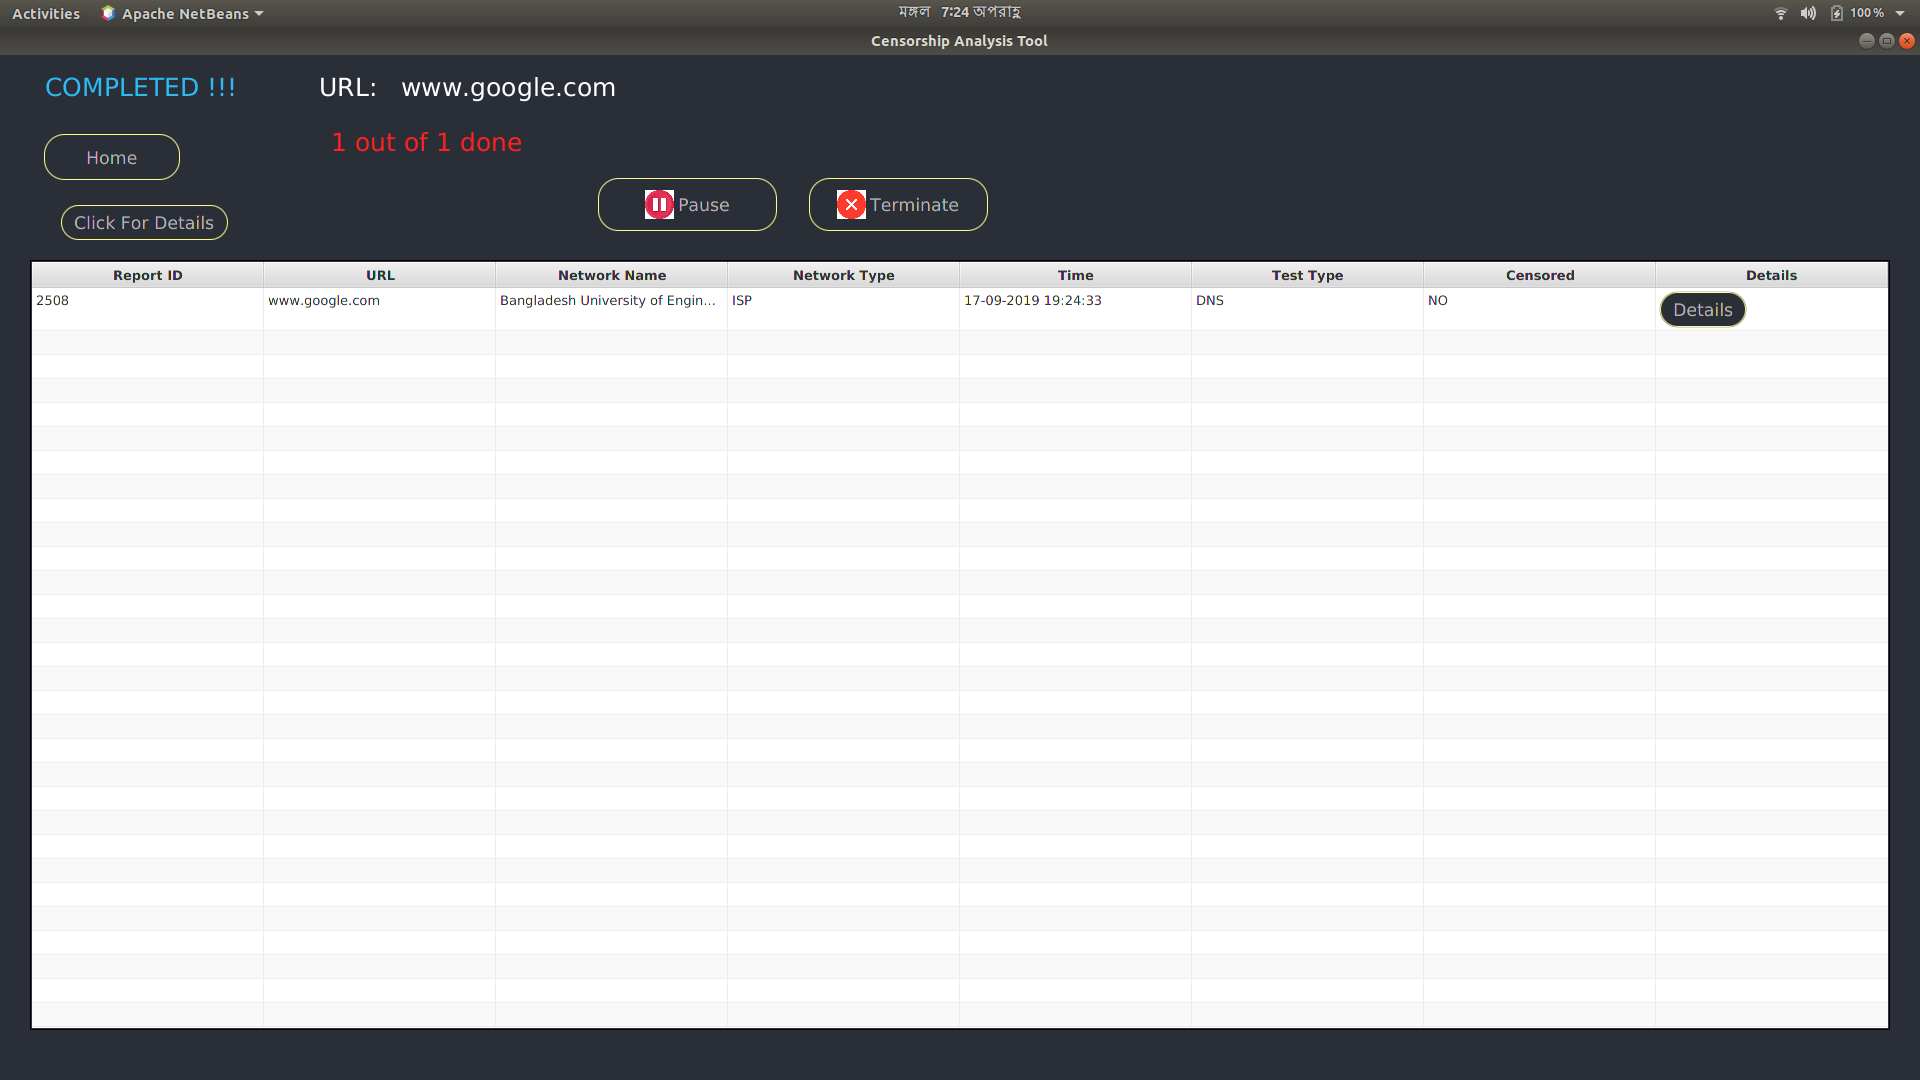
\includegraphics[width=\textwidth]{usersite/14completed.png}
    \caption{After completion of 1 test}
    \label{fig:user14}
\end{figure}

\begin{figure}[h]
    \centering
    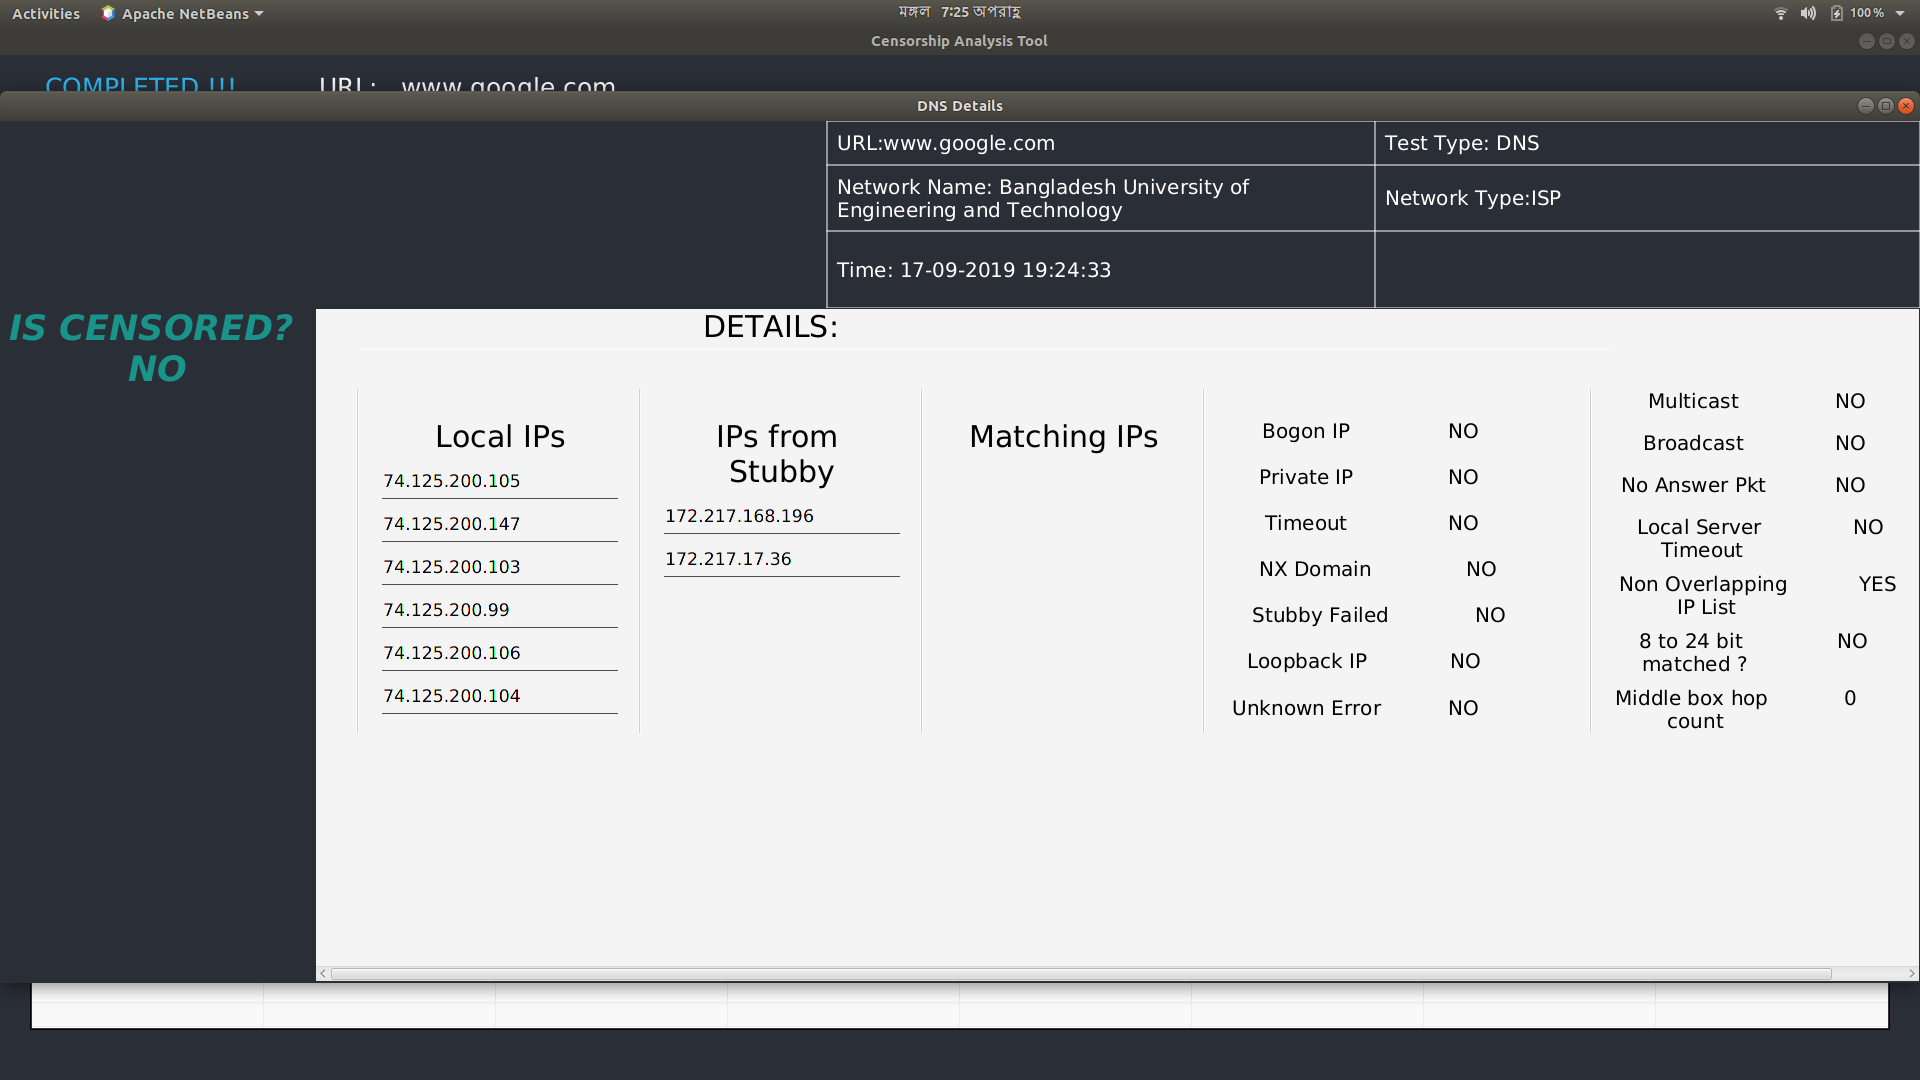
\includegraphics[width=\textwidth]{usersite/15details.png}
    \caption{After clicking details button}
    \label{fig:user15}
\end{figure}

\begin{figure}[h]
    \centering
    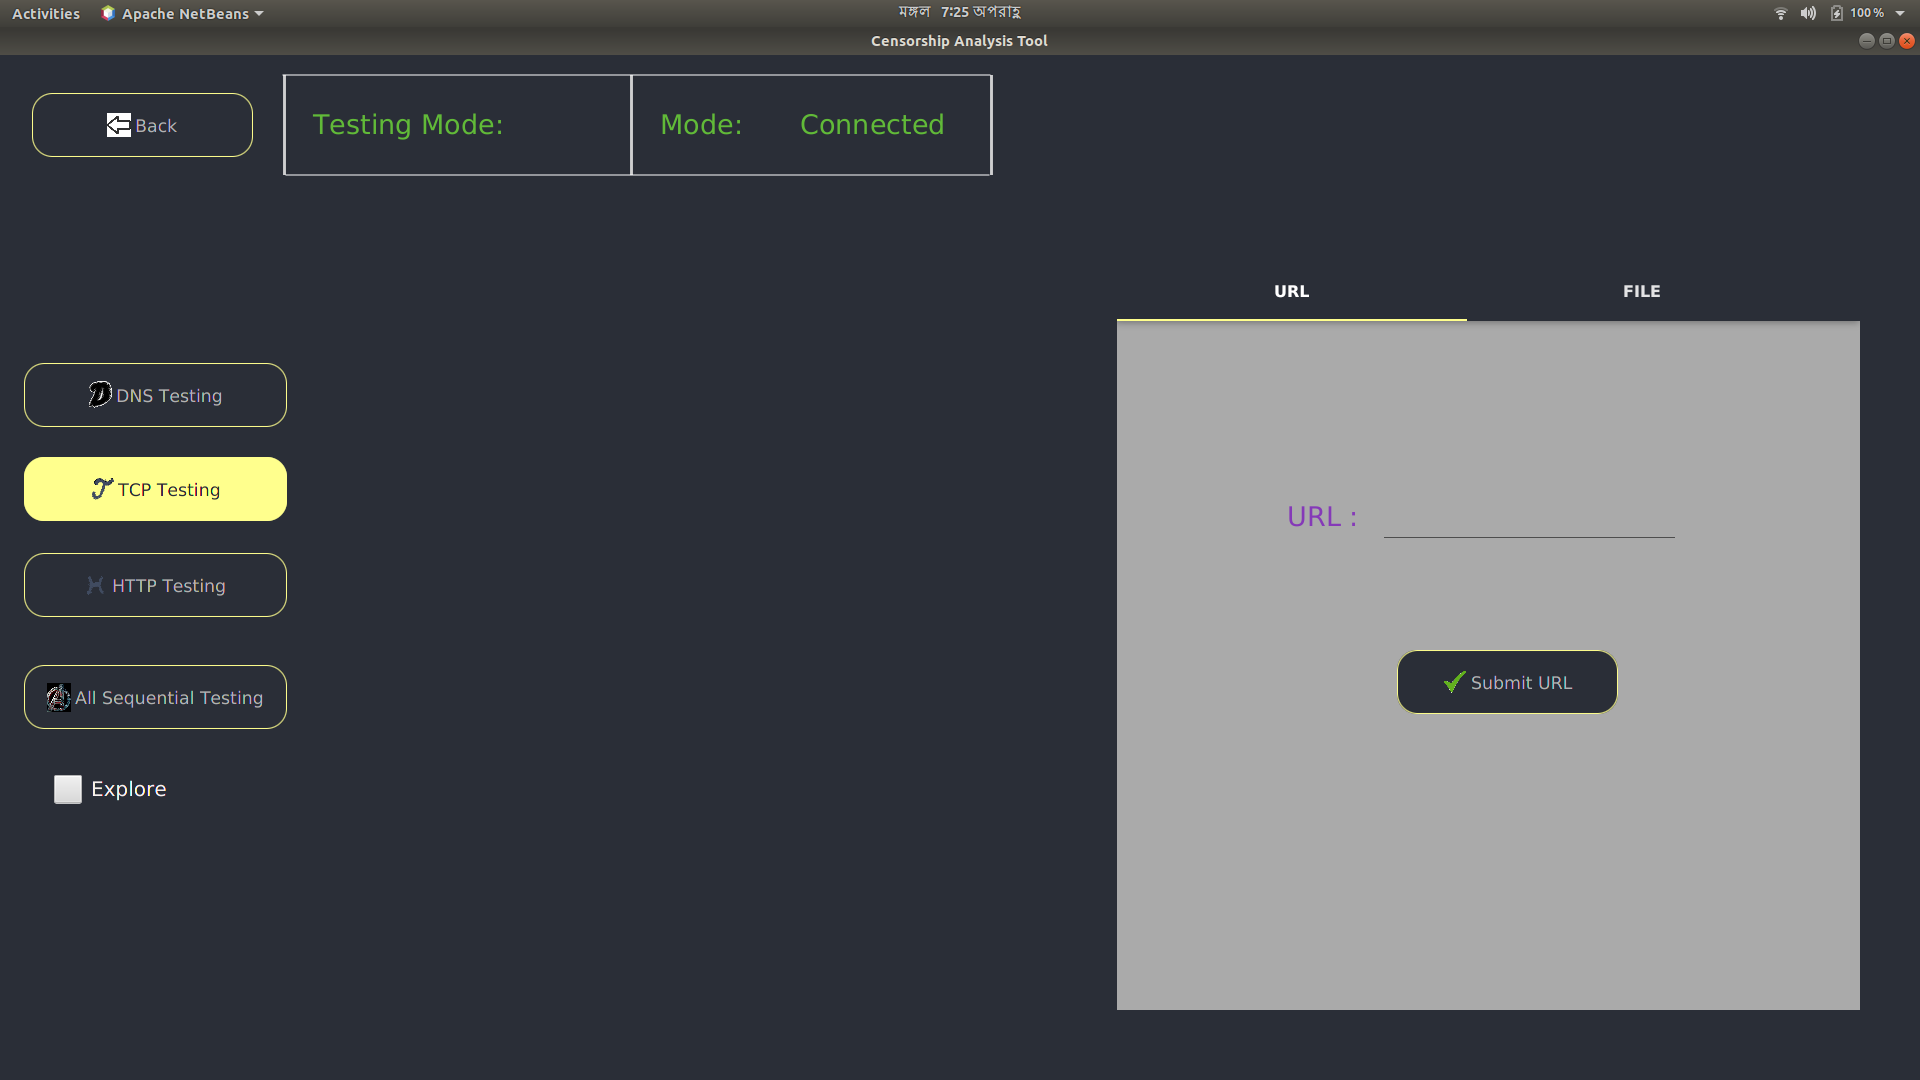
\includegraphics[width=\textwidth]{usersite/17tcptest.png}
    \caption{TCP Testing button is selected}
    \label{fig:user16}
\end{figure}

\begin{figure}[h]
    \centering
    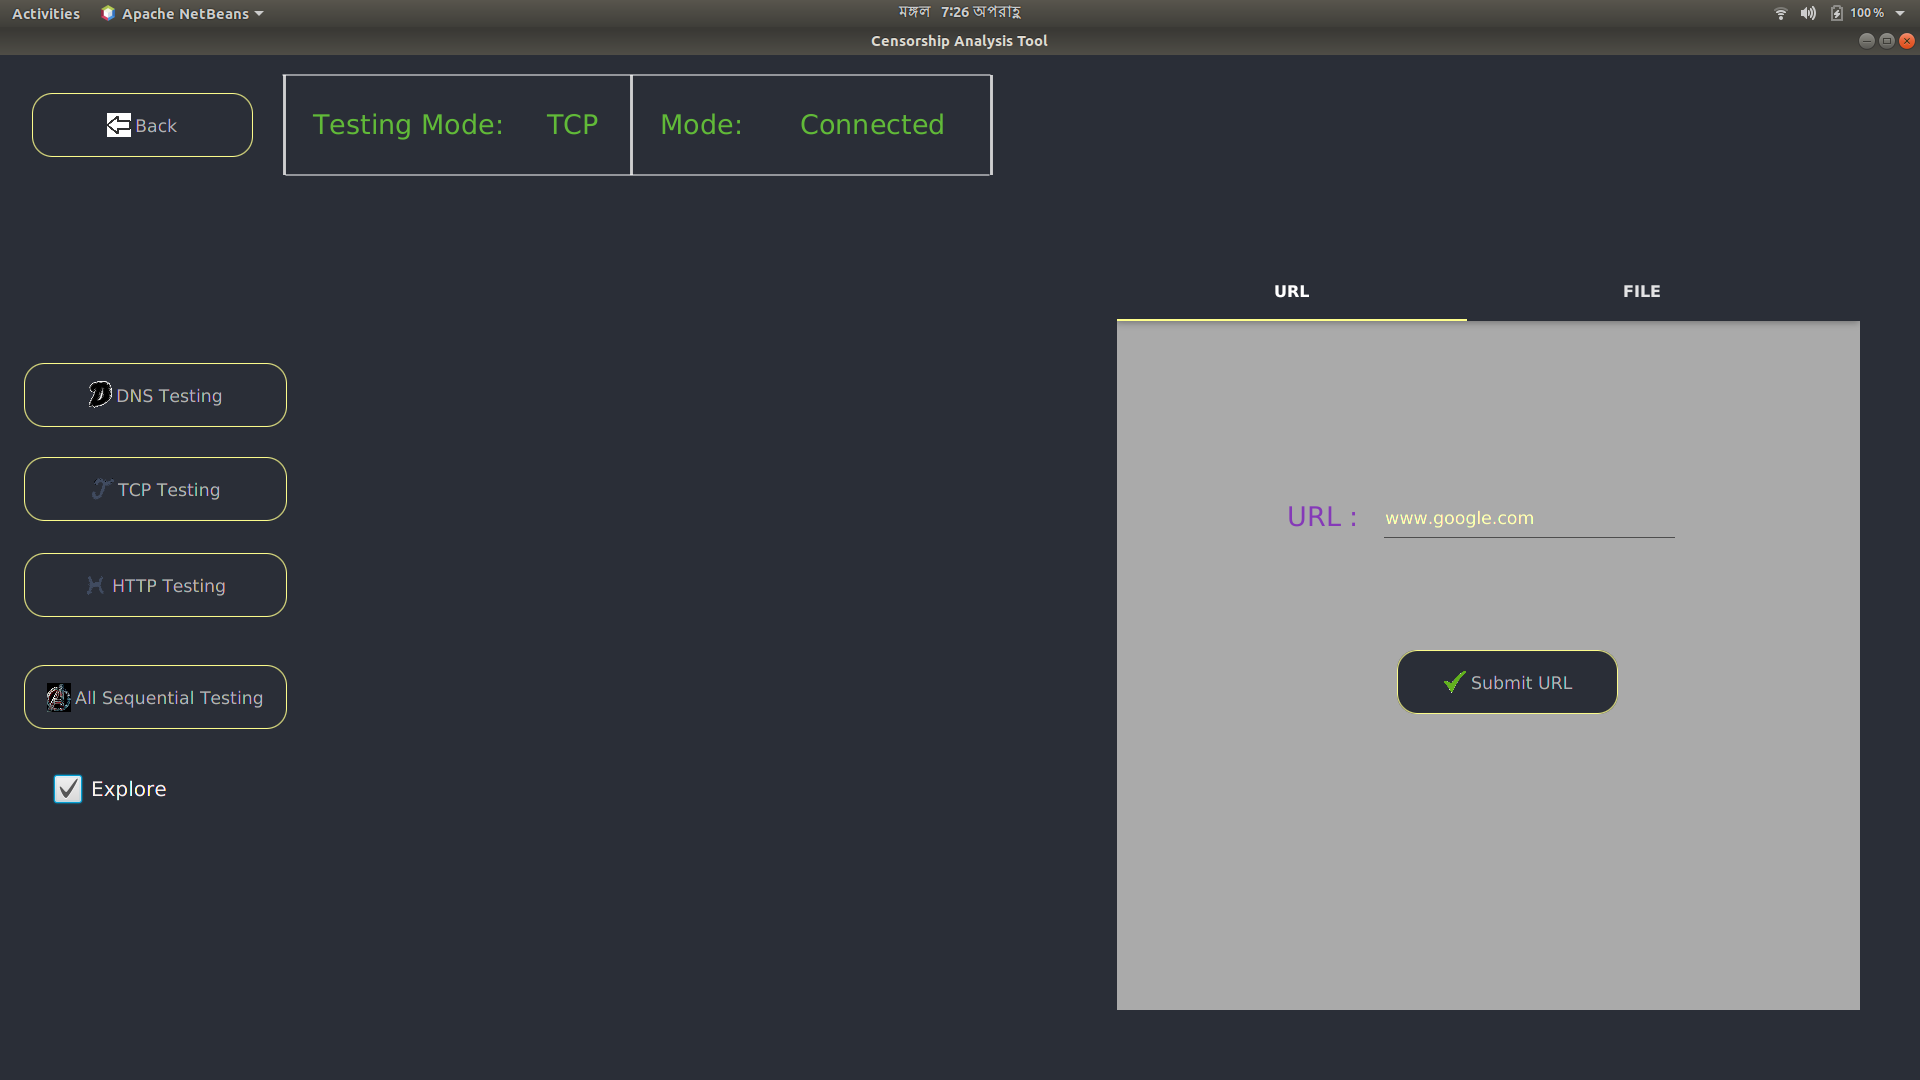
\includegraphics[width=\textwidth]{usersite/18tcptest2.png}
    \caption{TCP Testing input are given}
    \label{fig:user17}
\end{figure}

Real time underlying operation are given when a user click on \emph{Click for Details} button.

\begin{figure}[h]
    \centering
    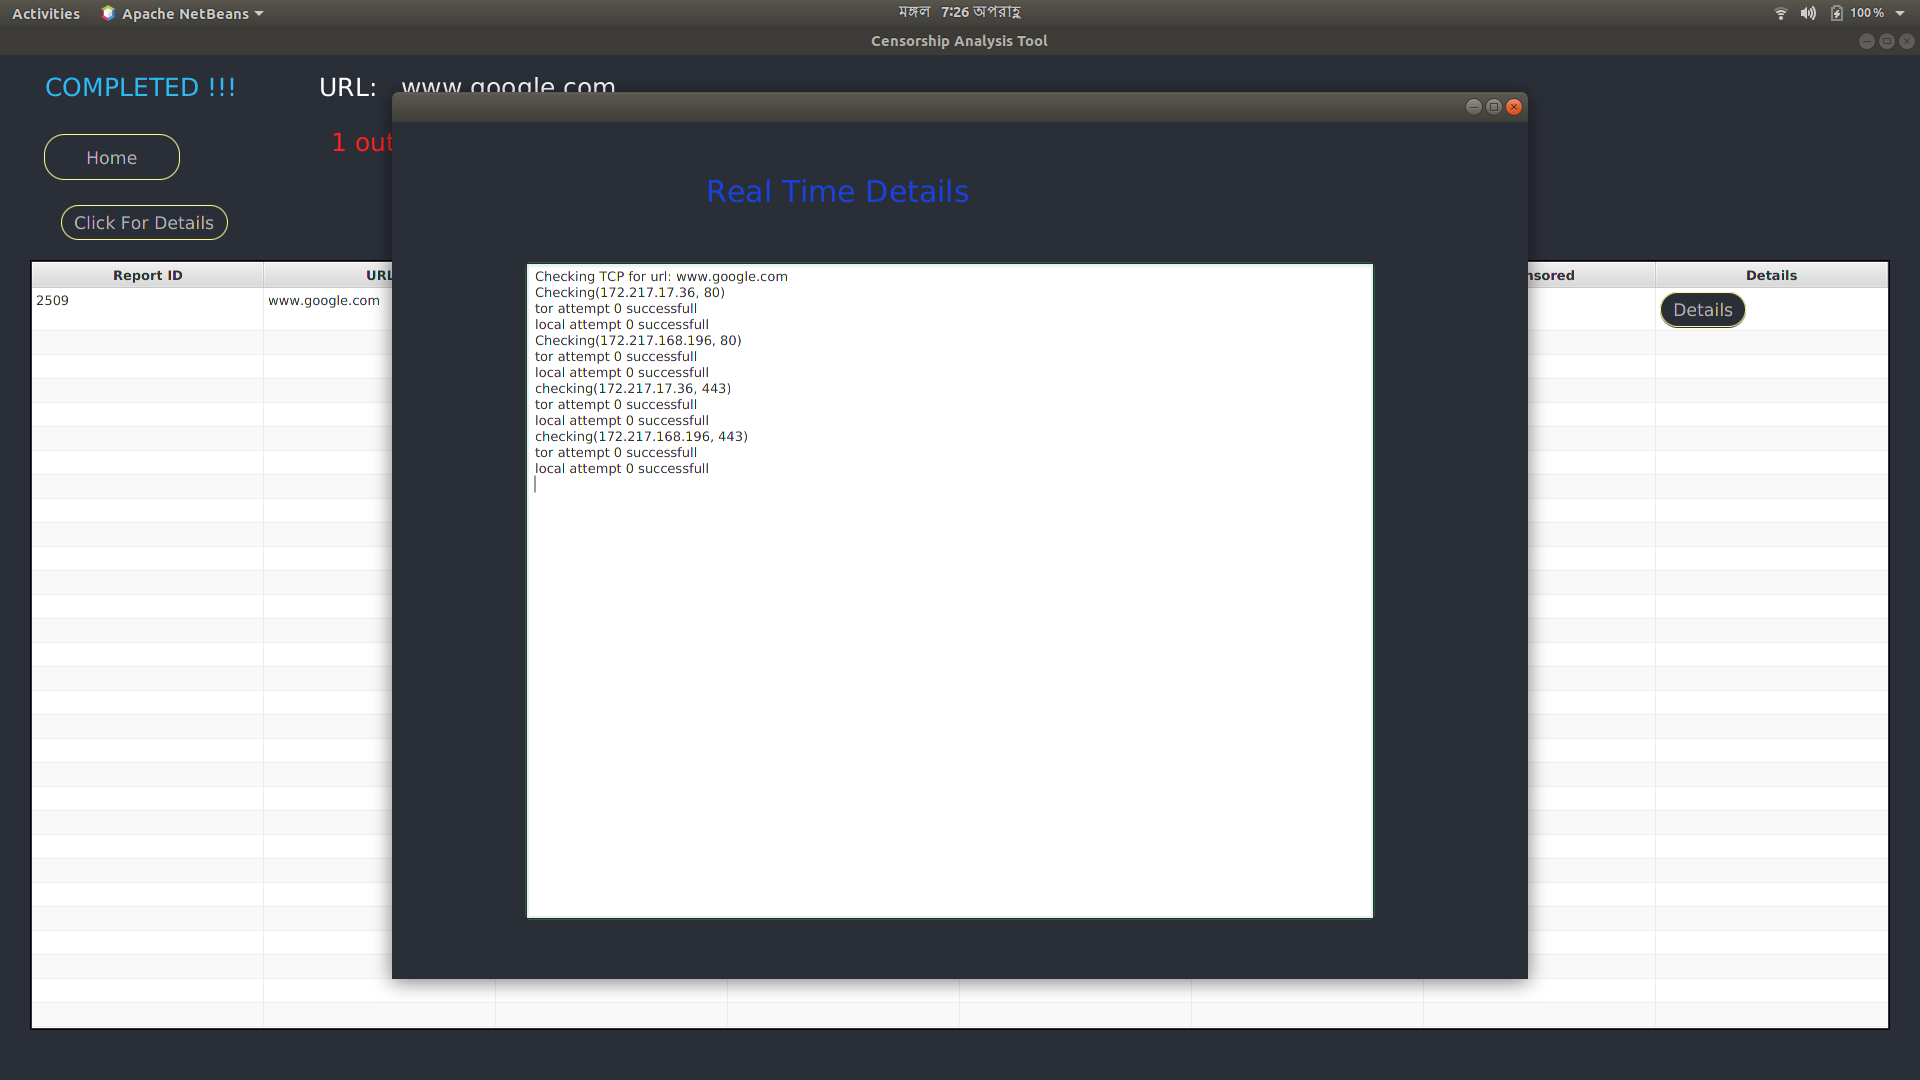
\includegraphics[width=\textwidth]{usersite/19realtime.png}
    \caption{After Click for Details button clicking real time data are shown }
    \label{fig:user18}
\end{figure}

\begin{figure}[h]
    \centering
    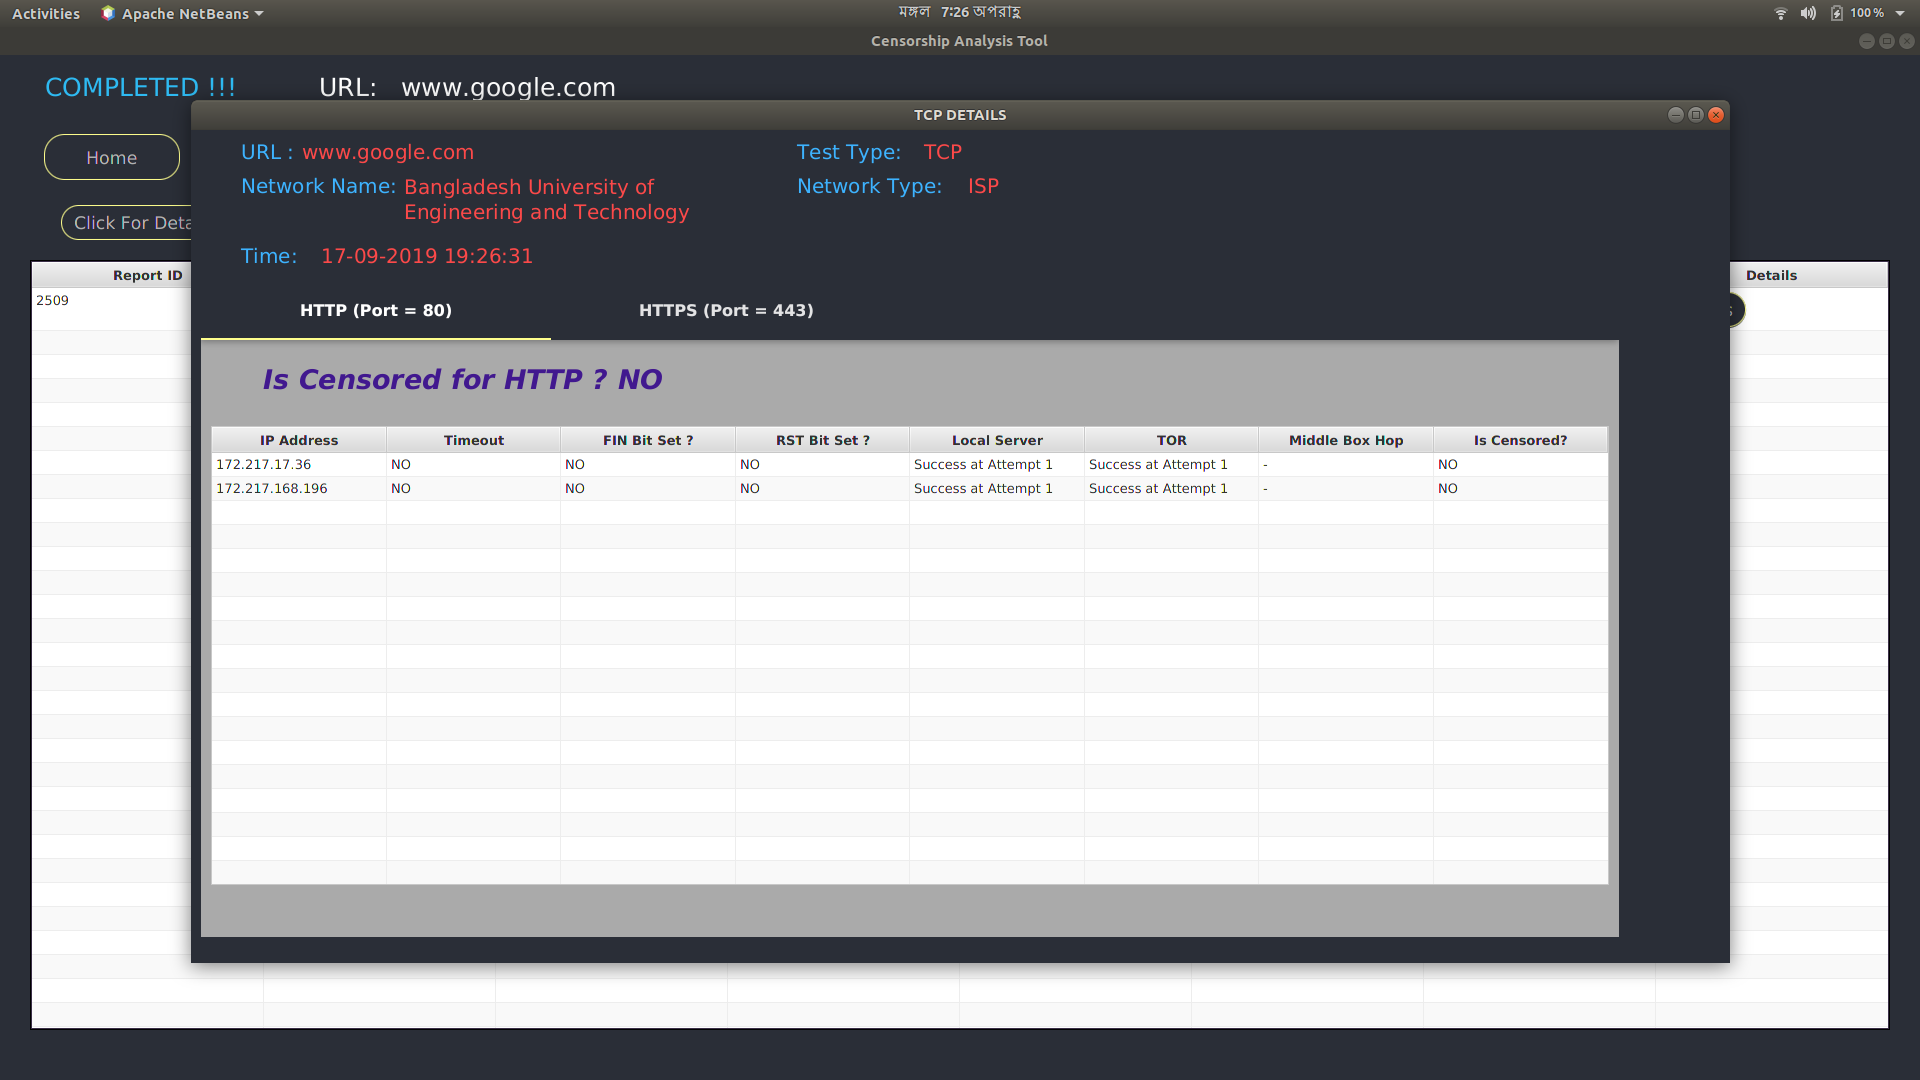
\includegraphics[width=\textwidth]{usersite/20tcpdetailshttp.png}
    \caption{HTTP port 80 details}
    \label{fig:user19}
\end{figure}

\begin{figure}[h]
    \centering
    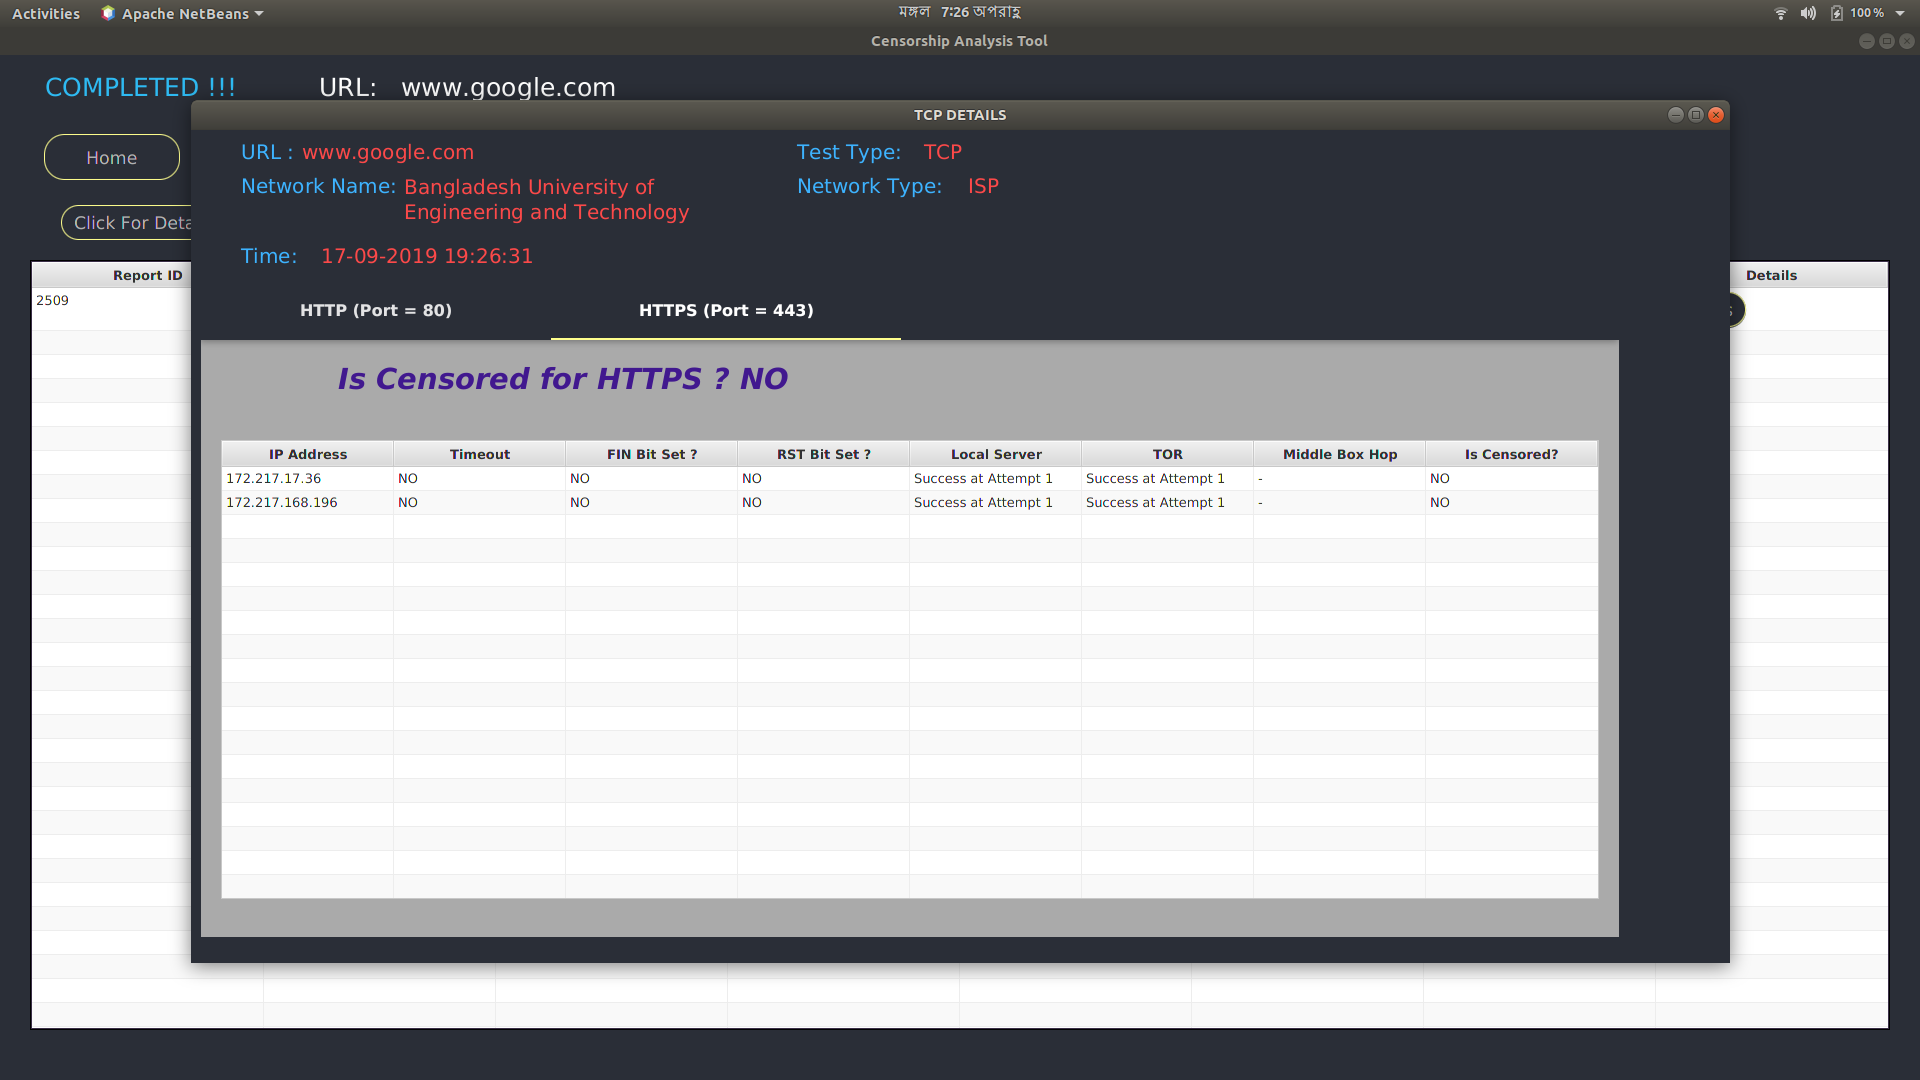
\includegraphics[width=\textwidth]{usersite/21tcpdetailshttps.png}
    \caption{HTTPS port 435 details}
    \label{fig:user20}
\end{figure}

\begin{figure}[h]
    \centering
    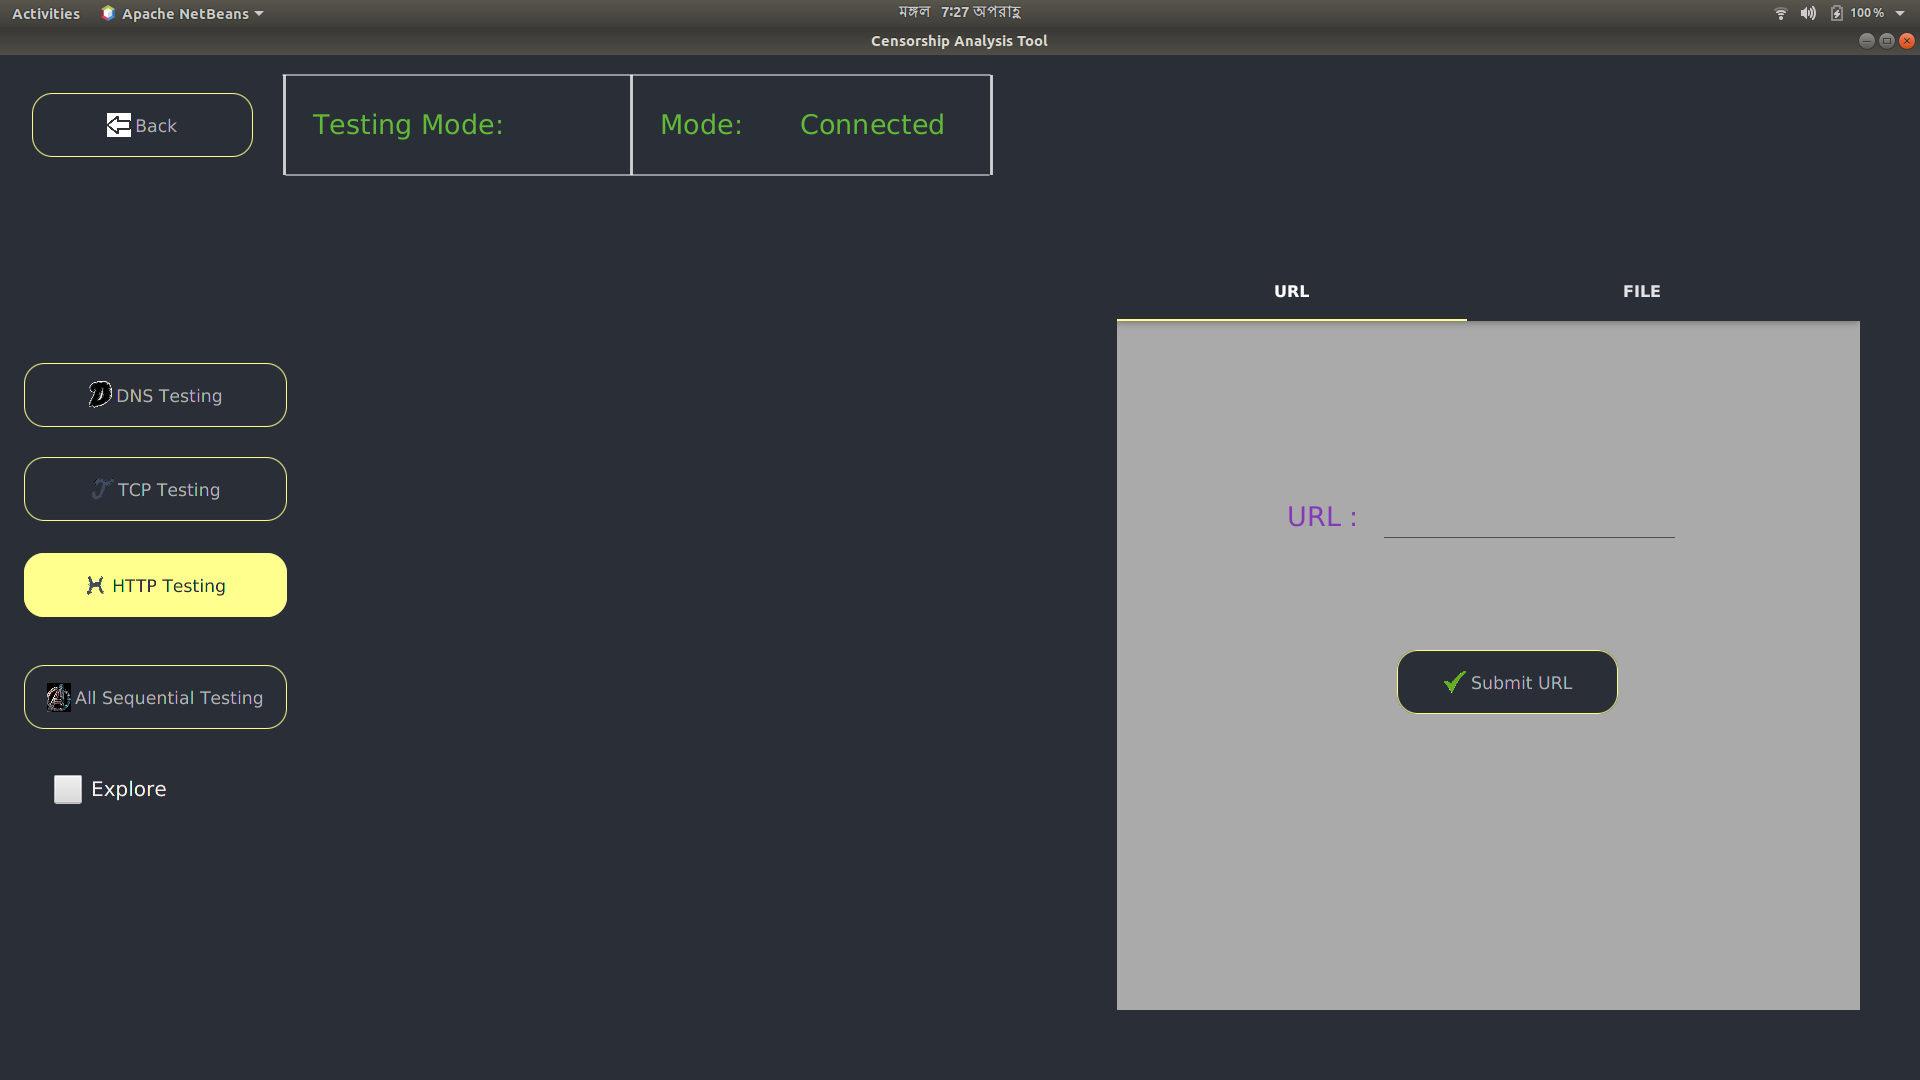
\includegraphics[width=\textwidth]{usersite/22httptest.png}
    \caption{HTTP Test button is clicked}
    \label{fig:user21}
\end{figure}

\begin{figure}[h]
    \centering
    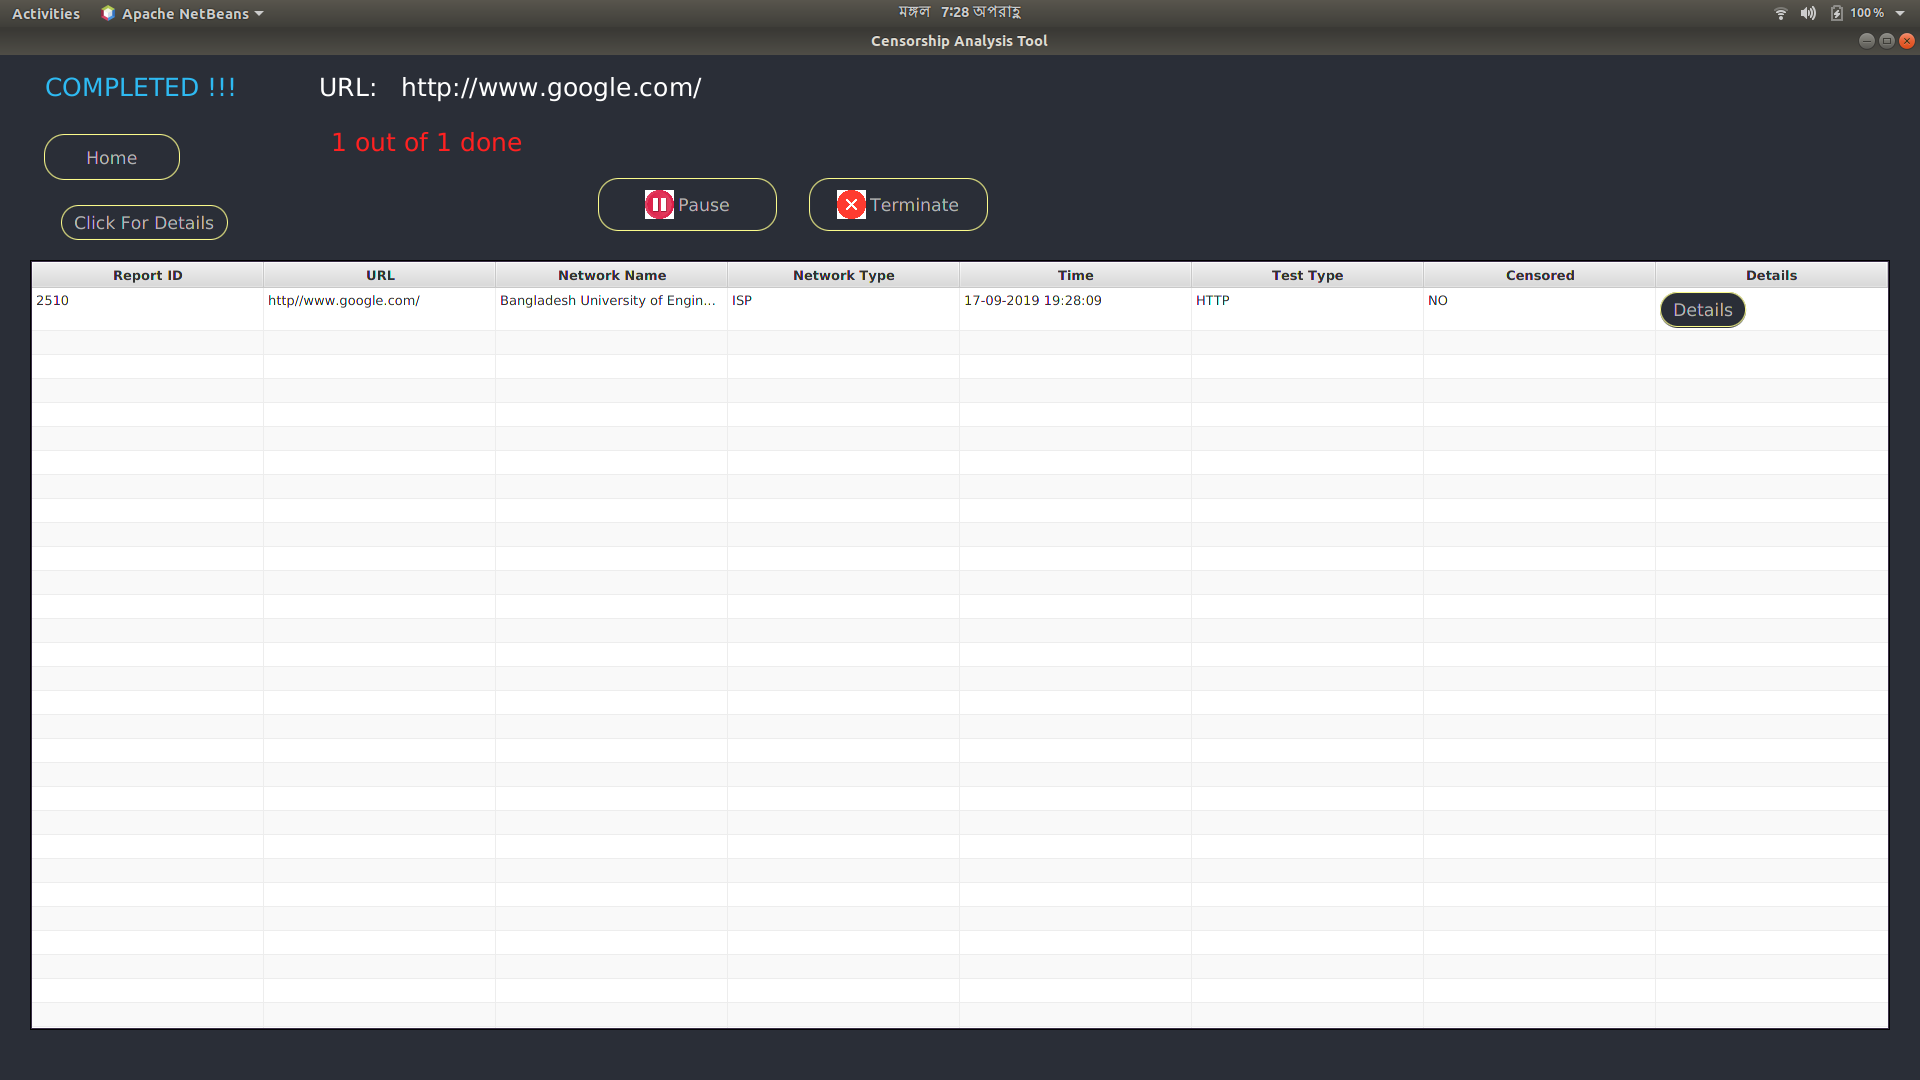
\includegraphics[width=\textwidth]{usersite/23httptestdone.png}
    \caption{HTTP Test done for 1 url}
    \label{fig:user22}
\end{figure}

\begin{figure}[h]
    \centering
    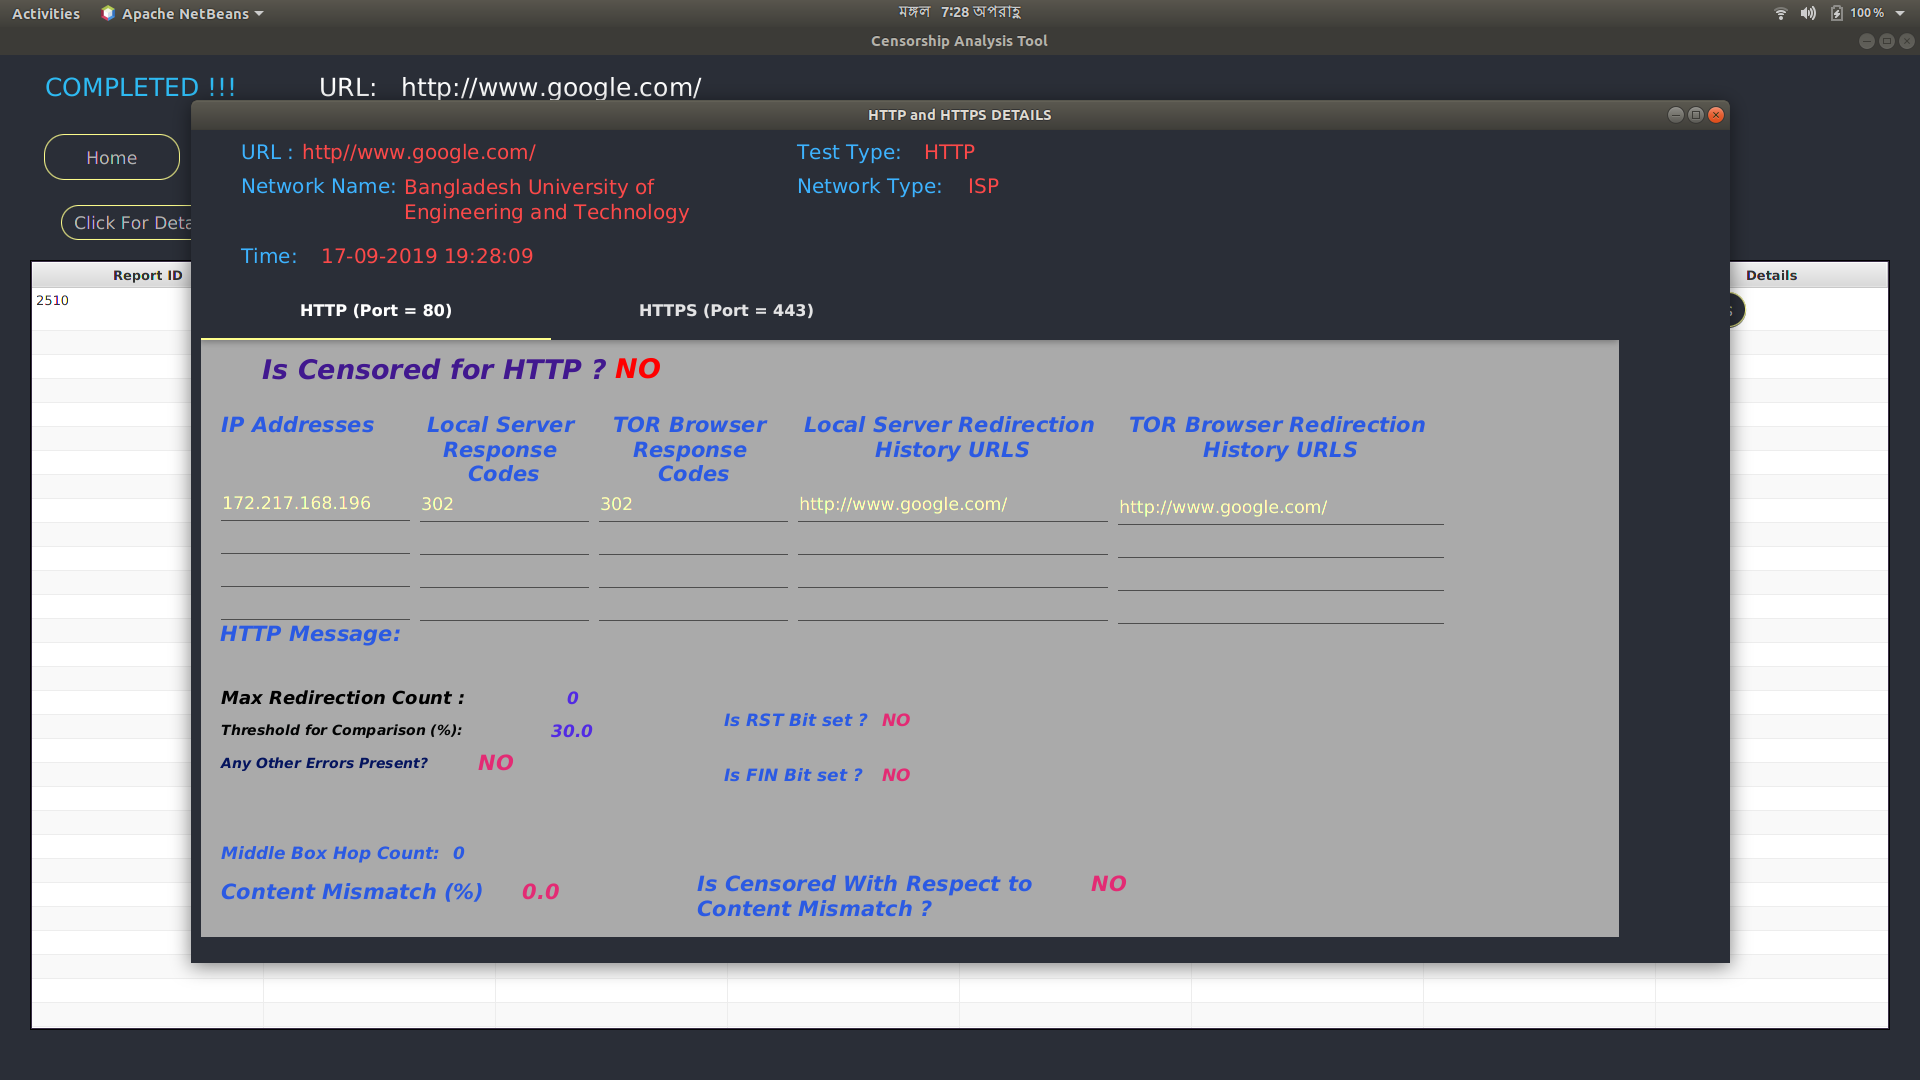
\includegraphics[width=\textwidth]{usersite/24httpdetails.png}
    \caption{HTTP port 80 details for HTTP test}
    \label{fig:user23}
\end{figure}

\begin{figure}[h]
    \centering
    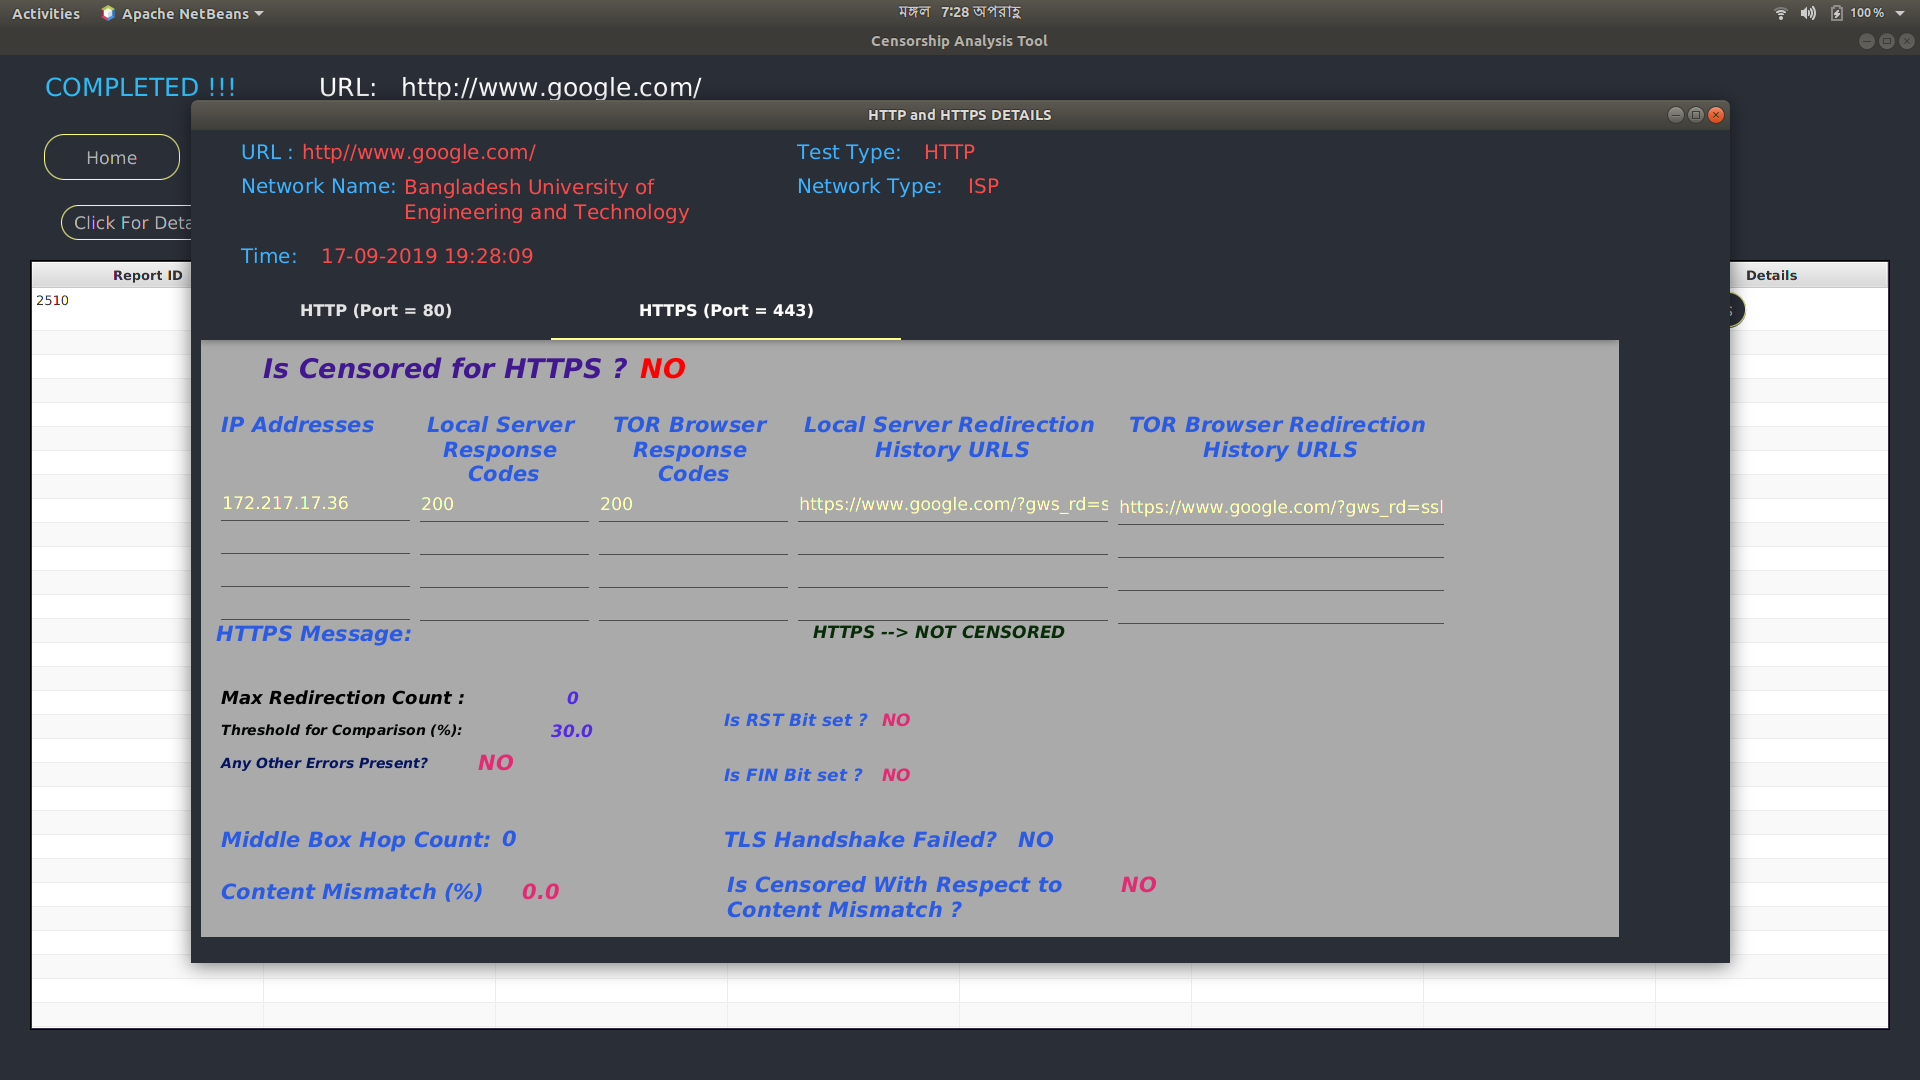
\includegraphics[width=\textwidth]{usersite/25httpsdetails.png}
    \caption{HTTPS port 435 details for HTTP test}
    \label{fig:user24}
\end{figure}

\begin{figure}[h]
    \centering
    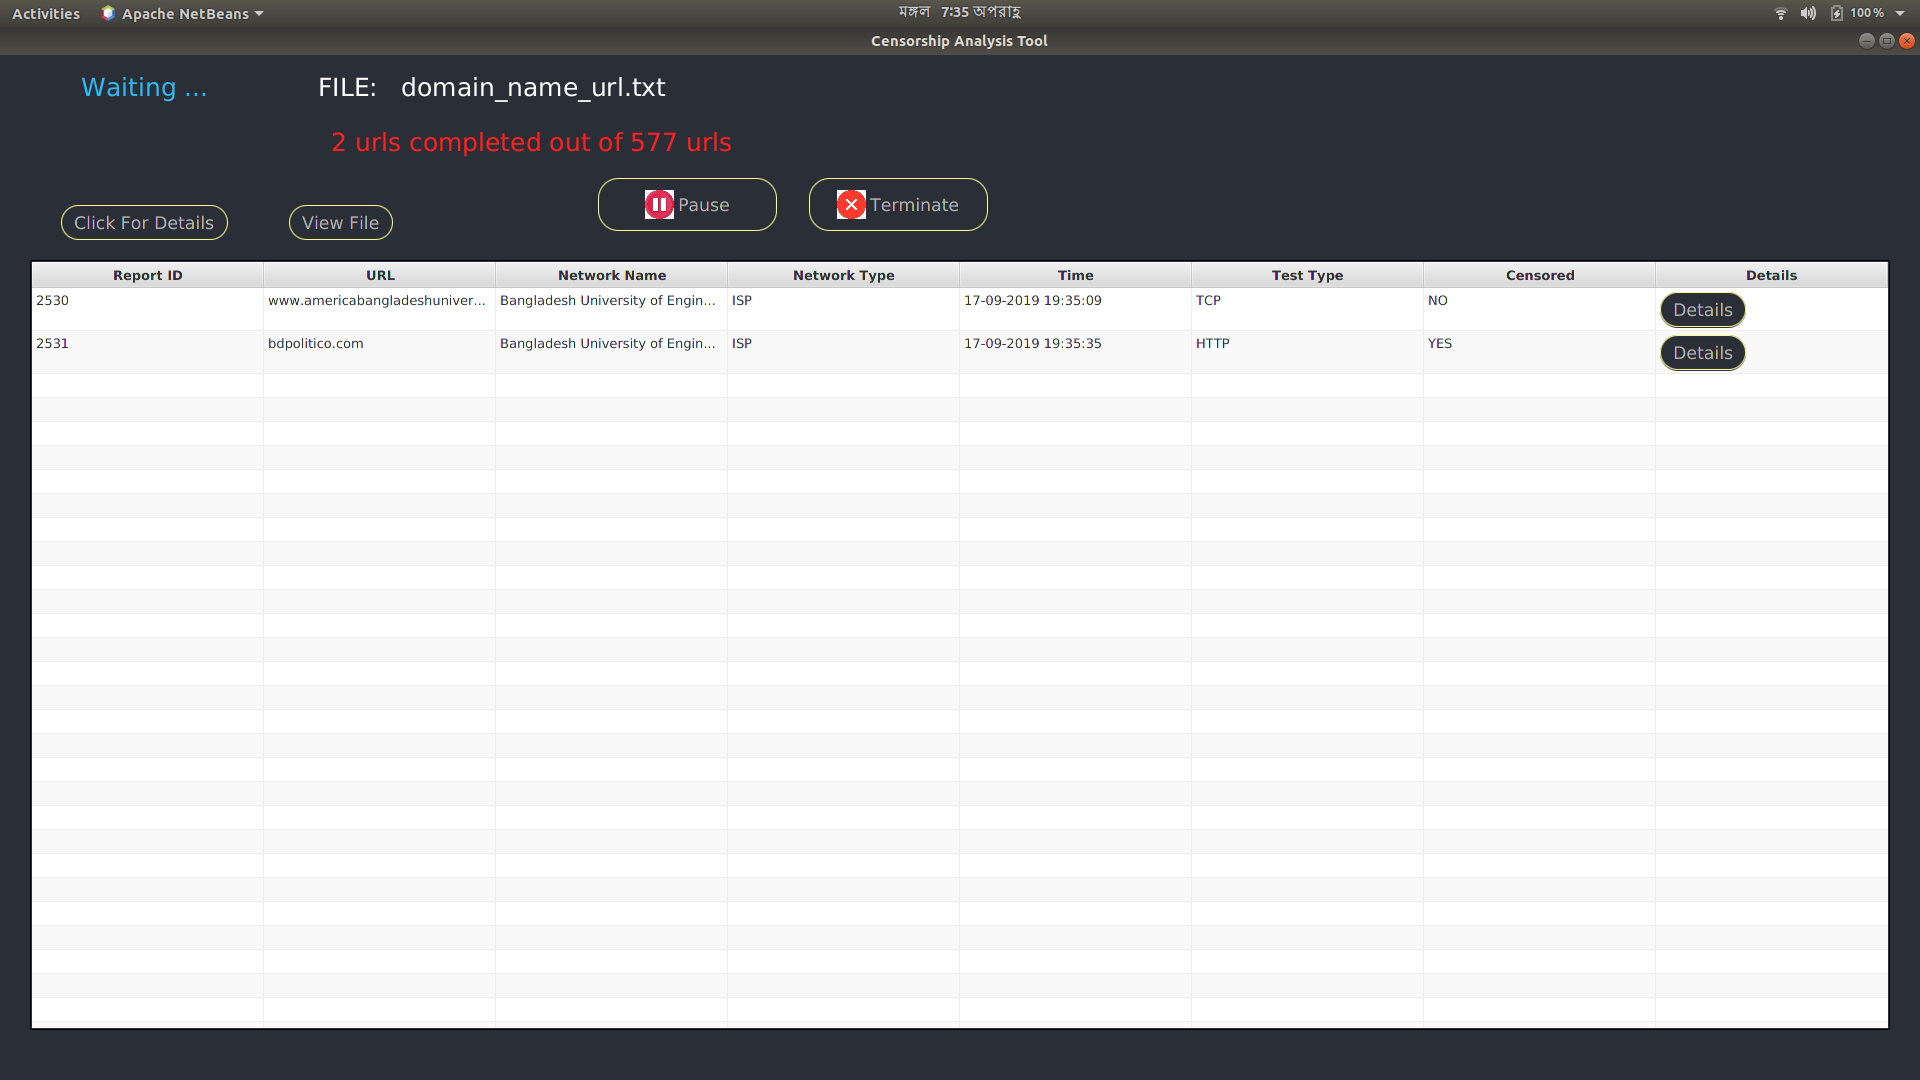
\includegraphics[width=\textwidth]{usersite/29filerunnin.png}
    \caption{A testing of file with urls started}
    \label{fig:user28}
\end{figure}


\begin{figure}[h]
    \centering
    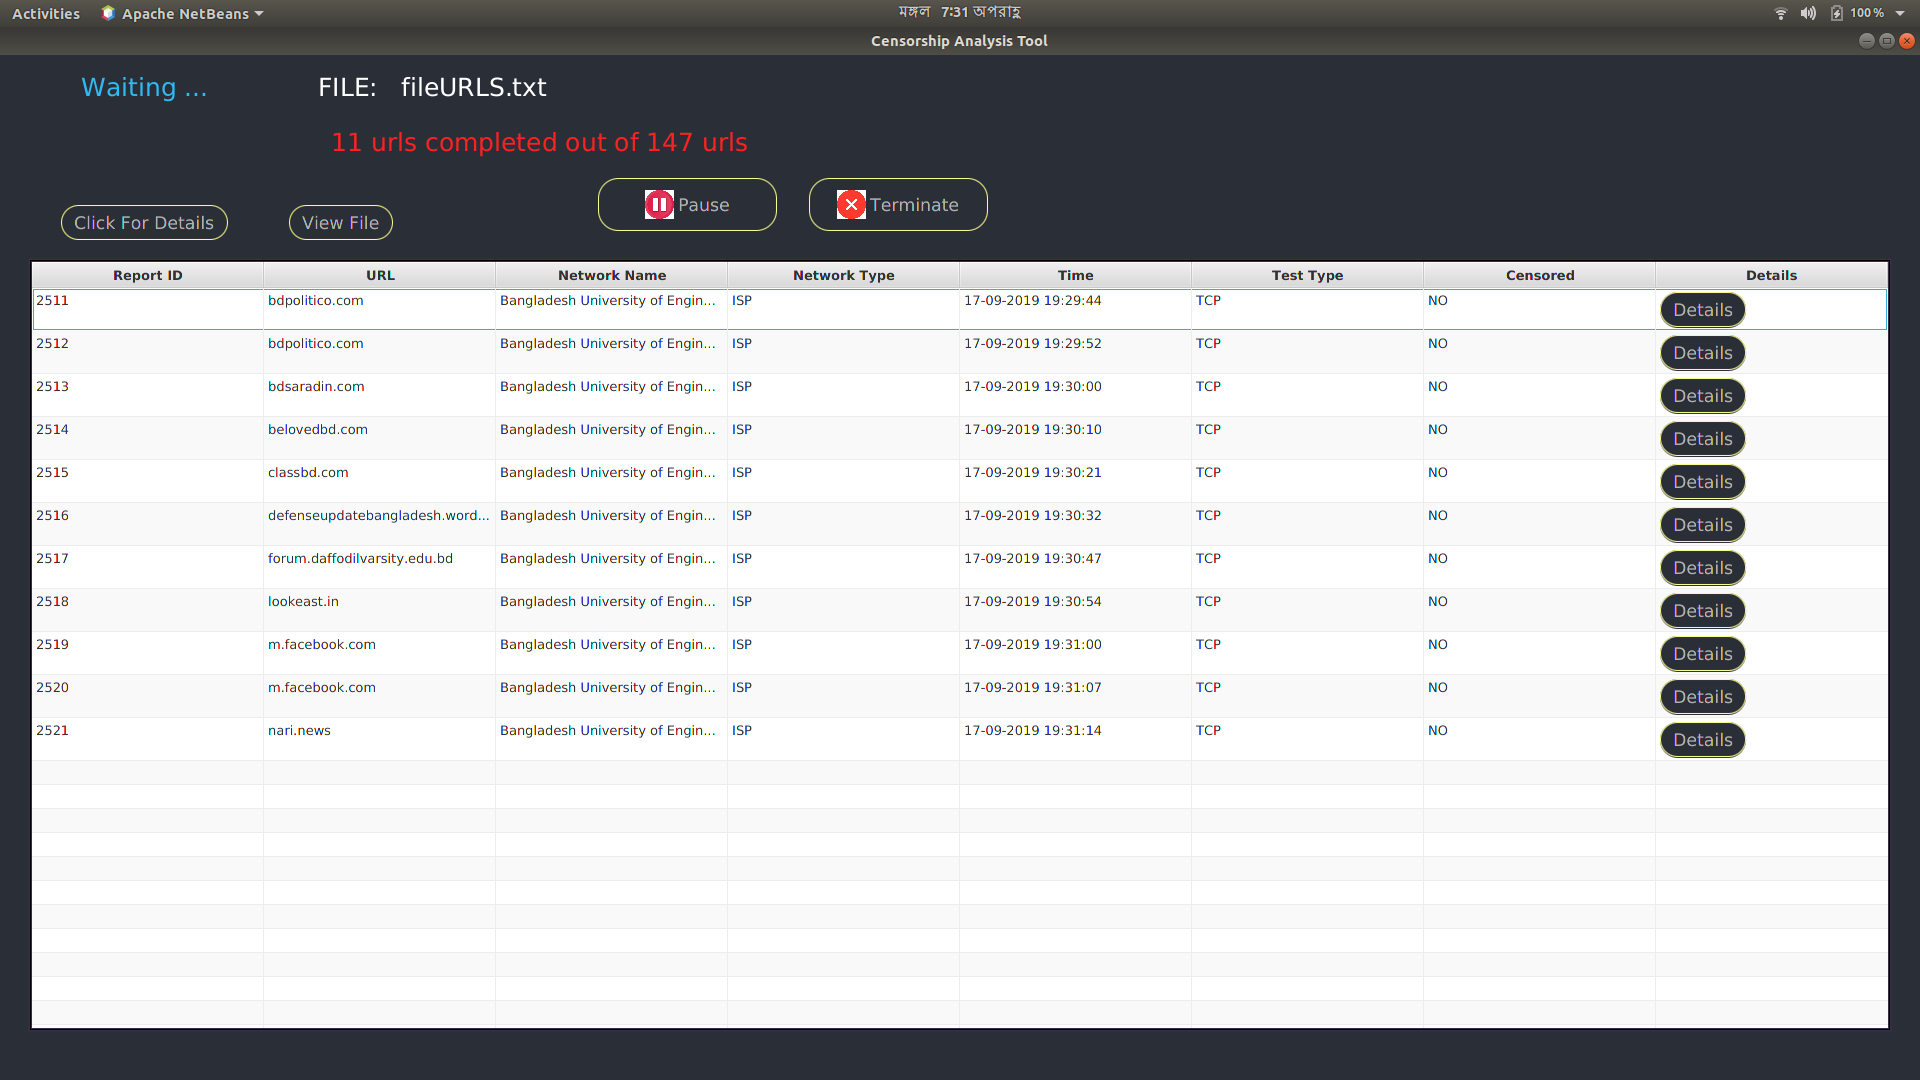
\includegraphics[width=\textwidth]{usersite/29filerunning.png}
    \caption{The testing of file with urls is going on}
    \label{fig:user29}
\end{figure}

\begin{figure}[h]
    \centering
    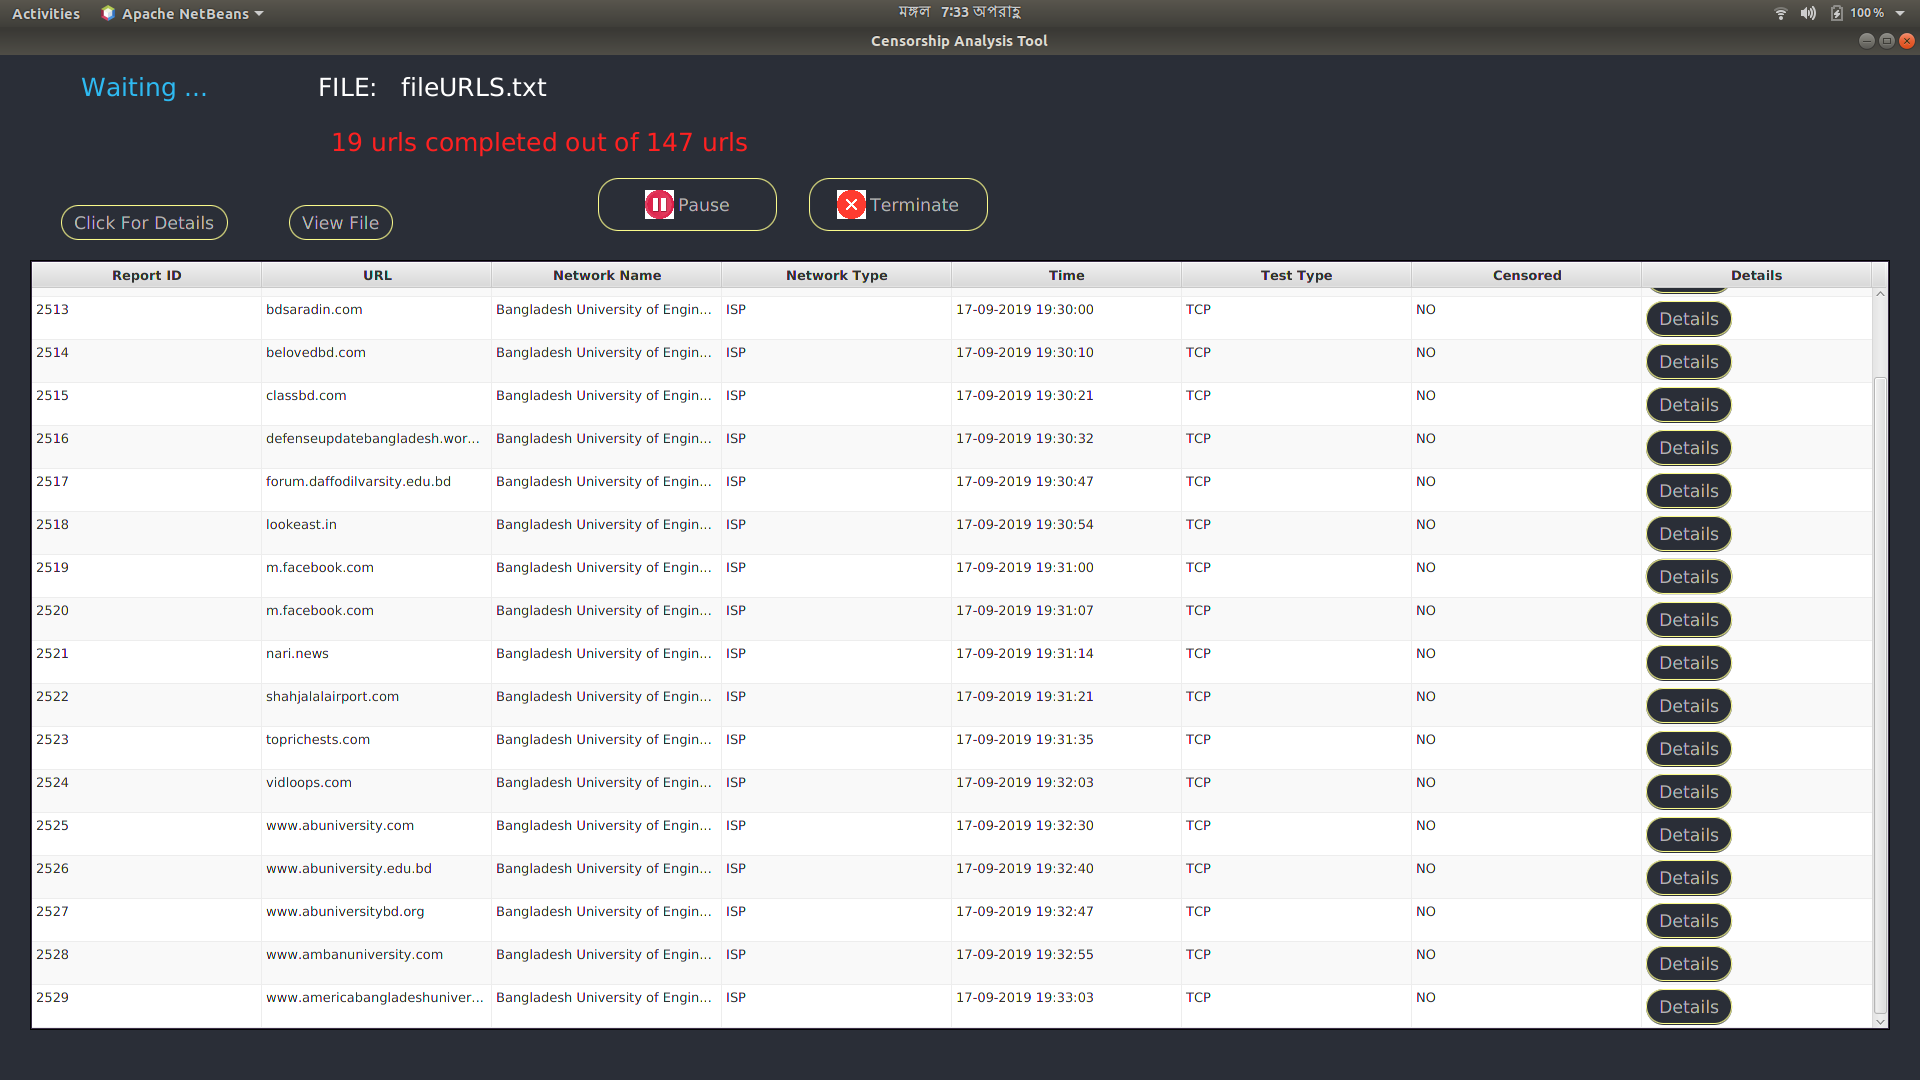
\includegraphics[width=\textwidth]{usersite/30filewaiting.png}
    \caption{The testing is going on}
    \label{fig:user30}
\end{figure}

\begin{figure}[h]
    \centering
    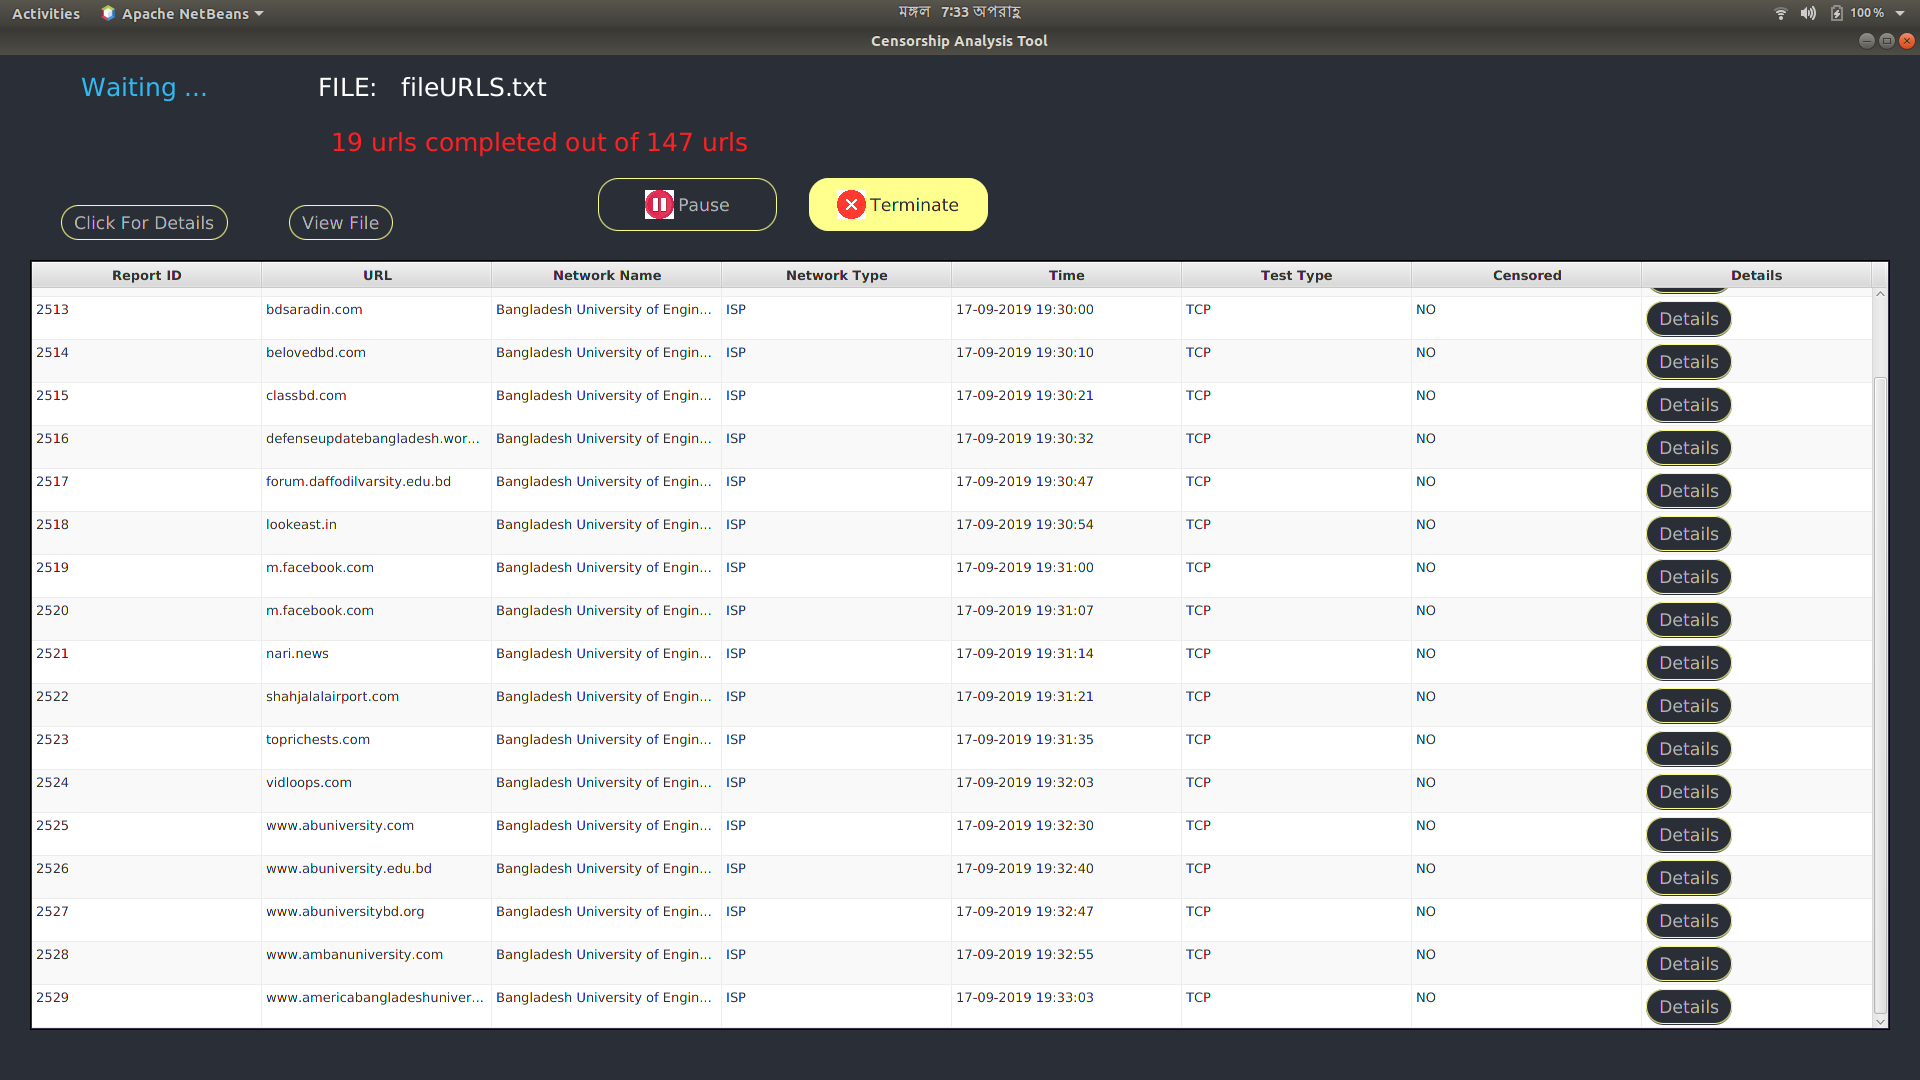
\includegraphics[width=\textwidth]{usersite/31filewaiting2.png}
    \caption{Terminating the test}
    \label{fig:user31}
\end{figure}

\begin{figure}[h]
    \centering
    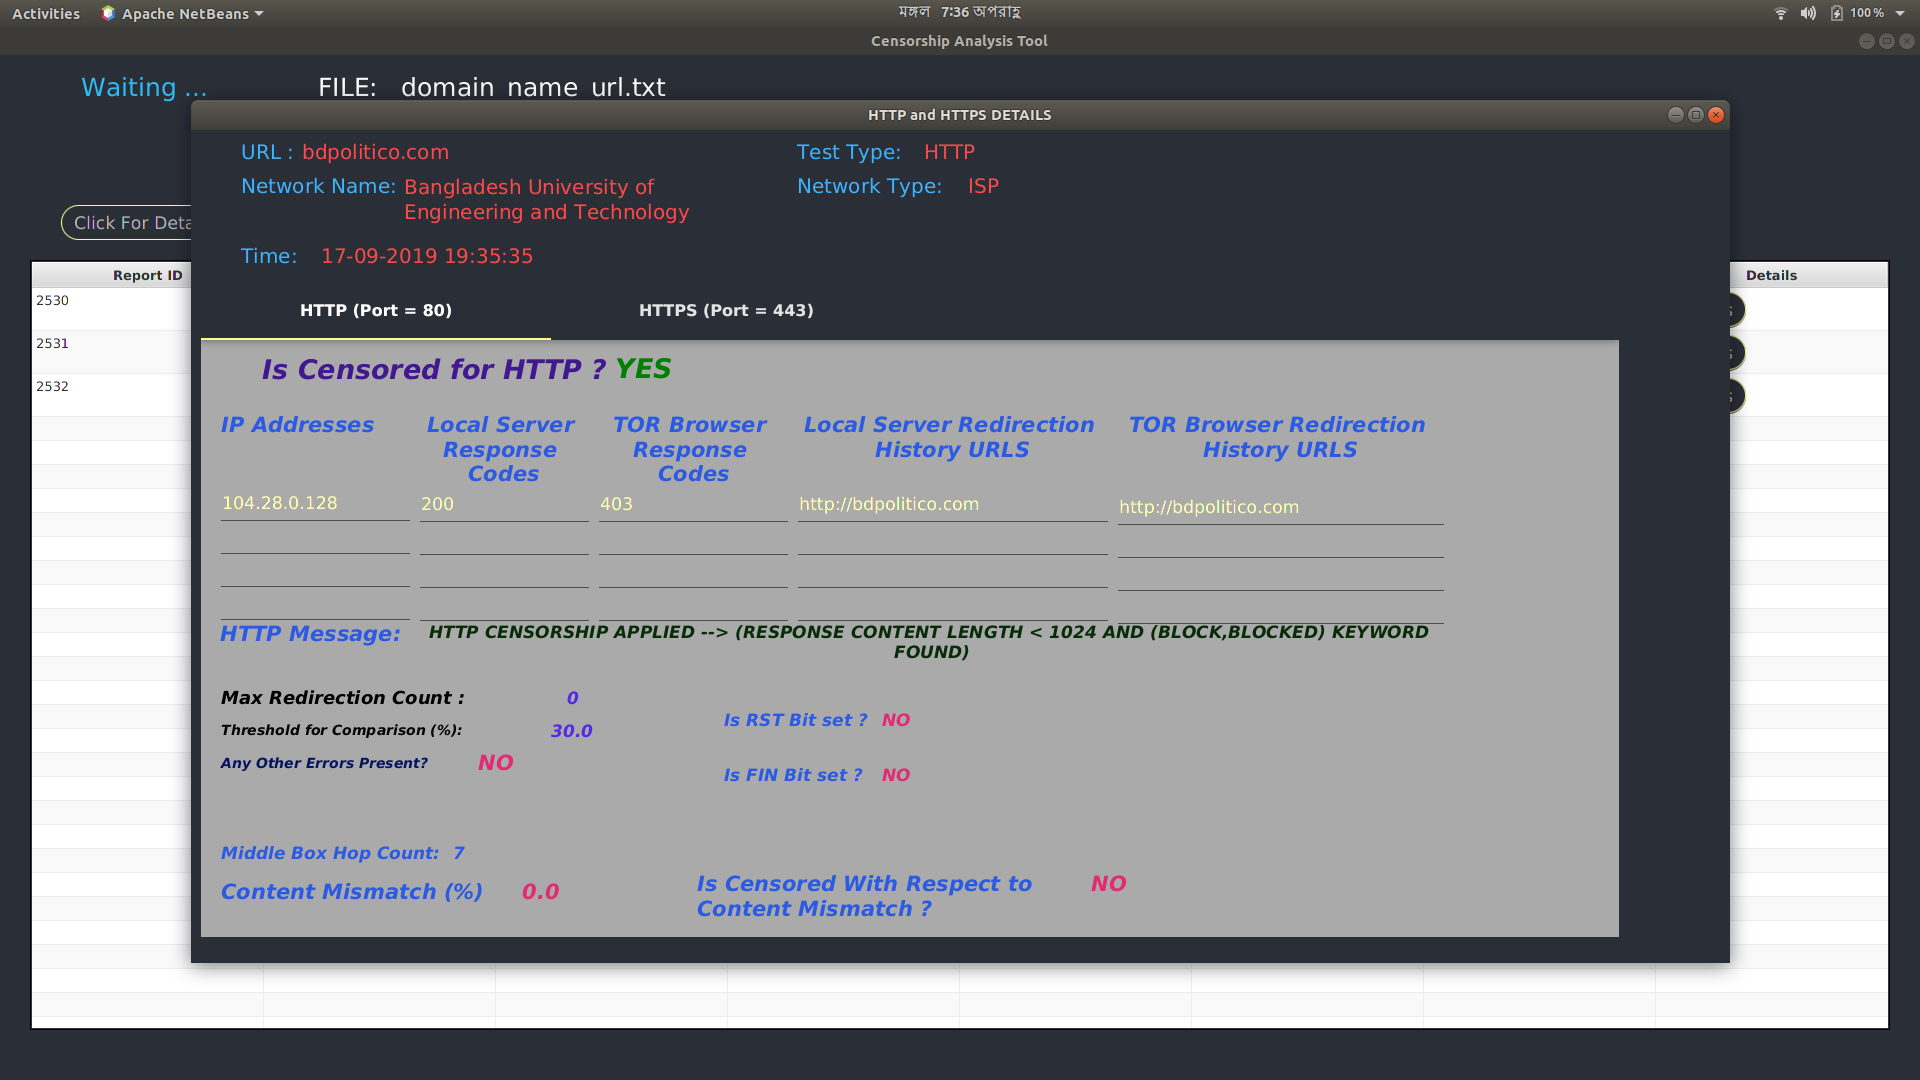
\includegraphics[width=\textwidth]{usersite/32httpdetails.png}
    \caption{HTTP port 80 data are seen}
    \label{fig:user32}
\end{figure}



\begin{figure}[h]
    \centering
    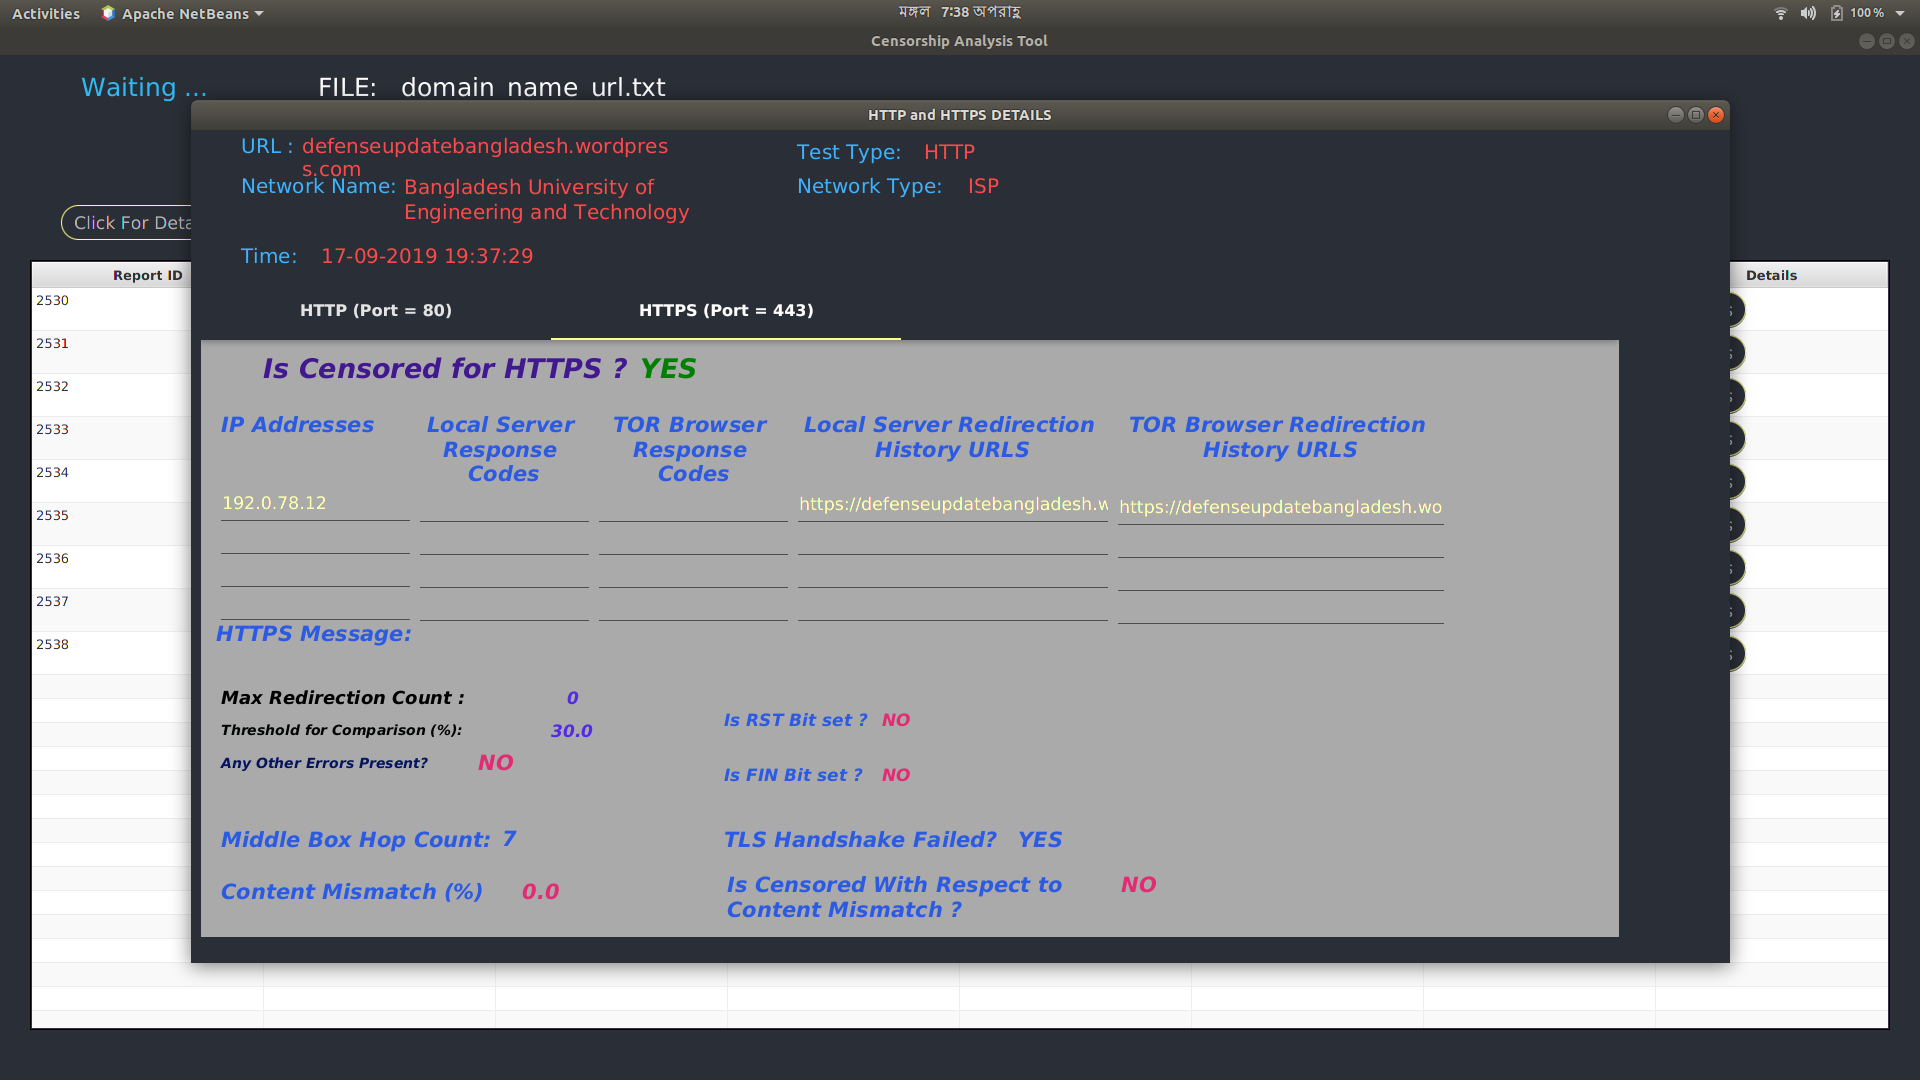
\includegraphics[width=\textwidth]{usersite/34httpsrealtime.png}
    \caption{HTTPS port 435 data are seen}
    \label{fig:user34}
\end{figure}

\begin{figure}[h]
    \centering
    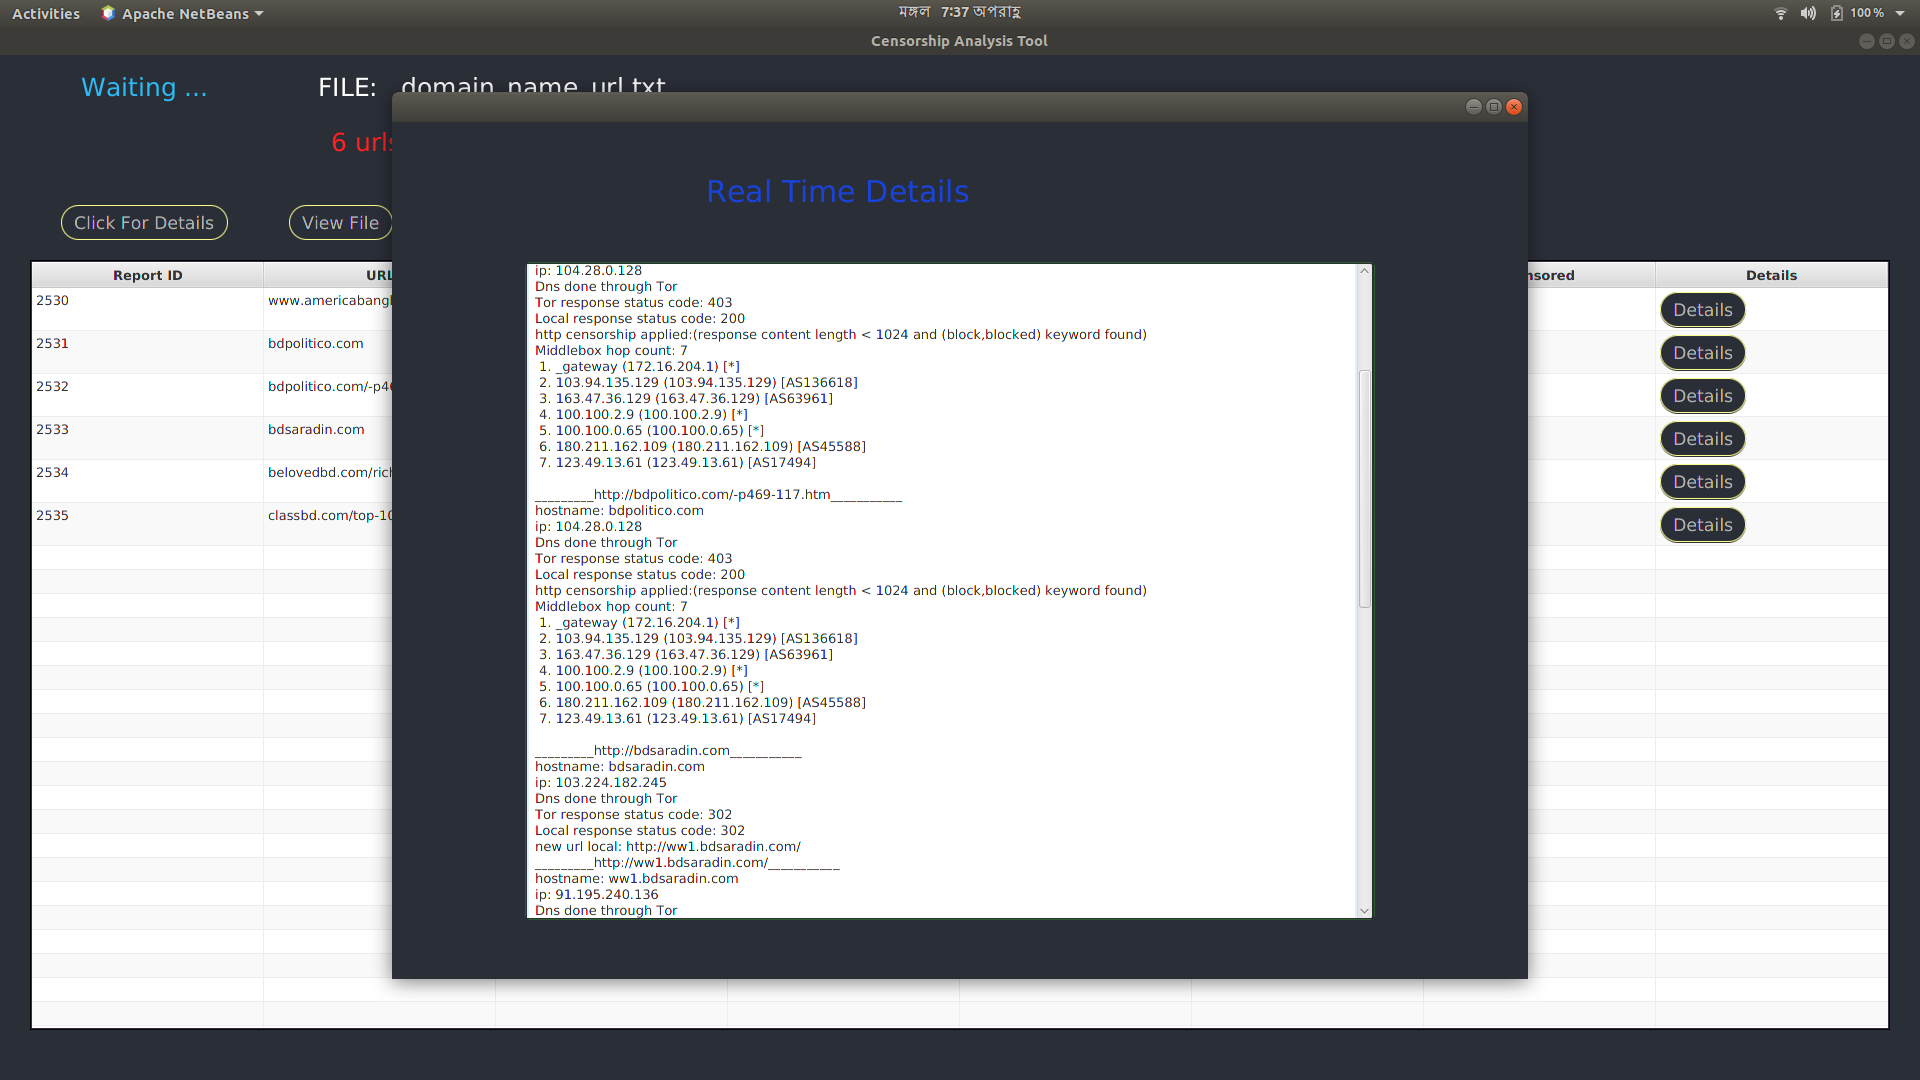
\includegraphics[width=\textwidth]{usersite/33httprealtime.png}
    \caption{HTTP real time operations}
    \label{fig:user33}
\end{figure}

\begin{figure}[h]
    \centering
    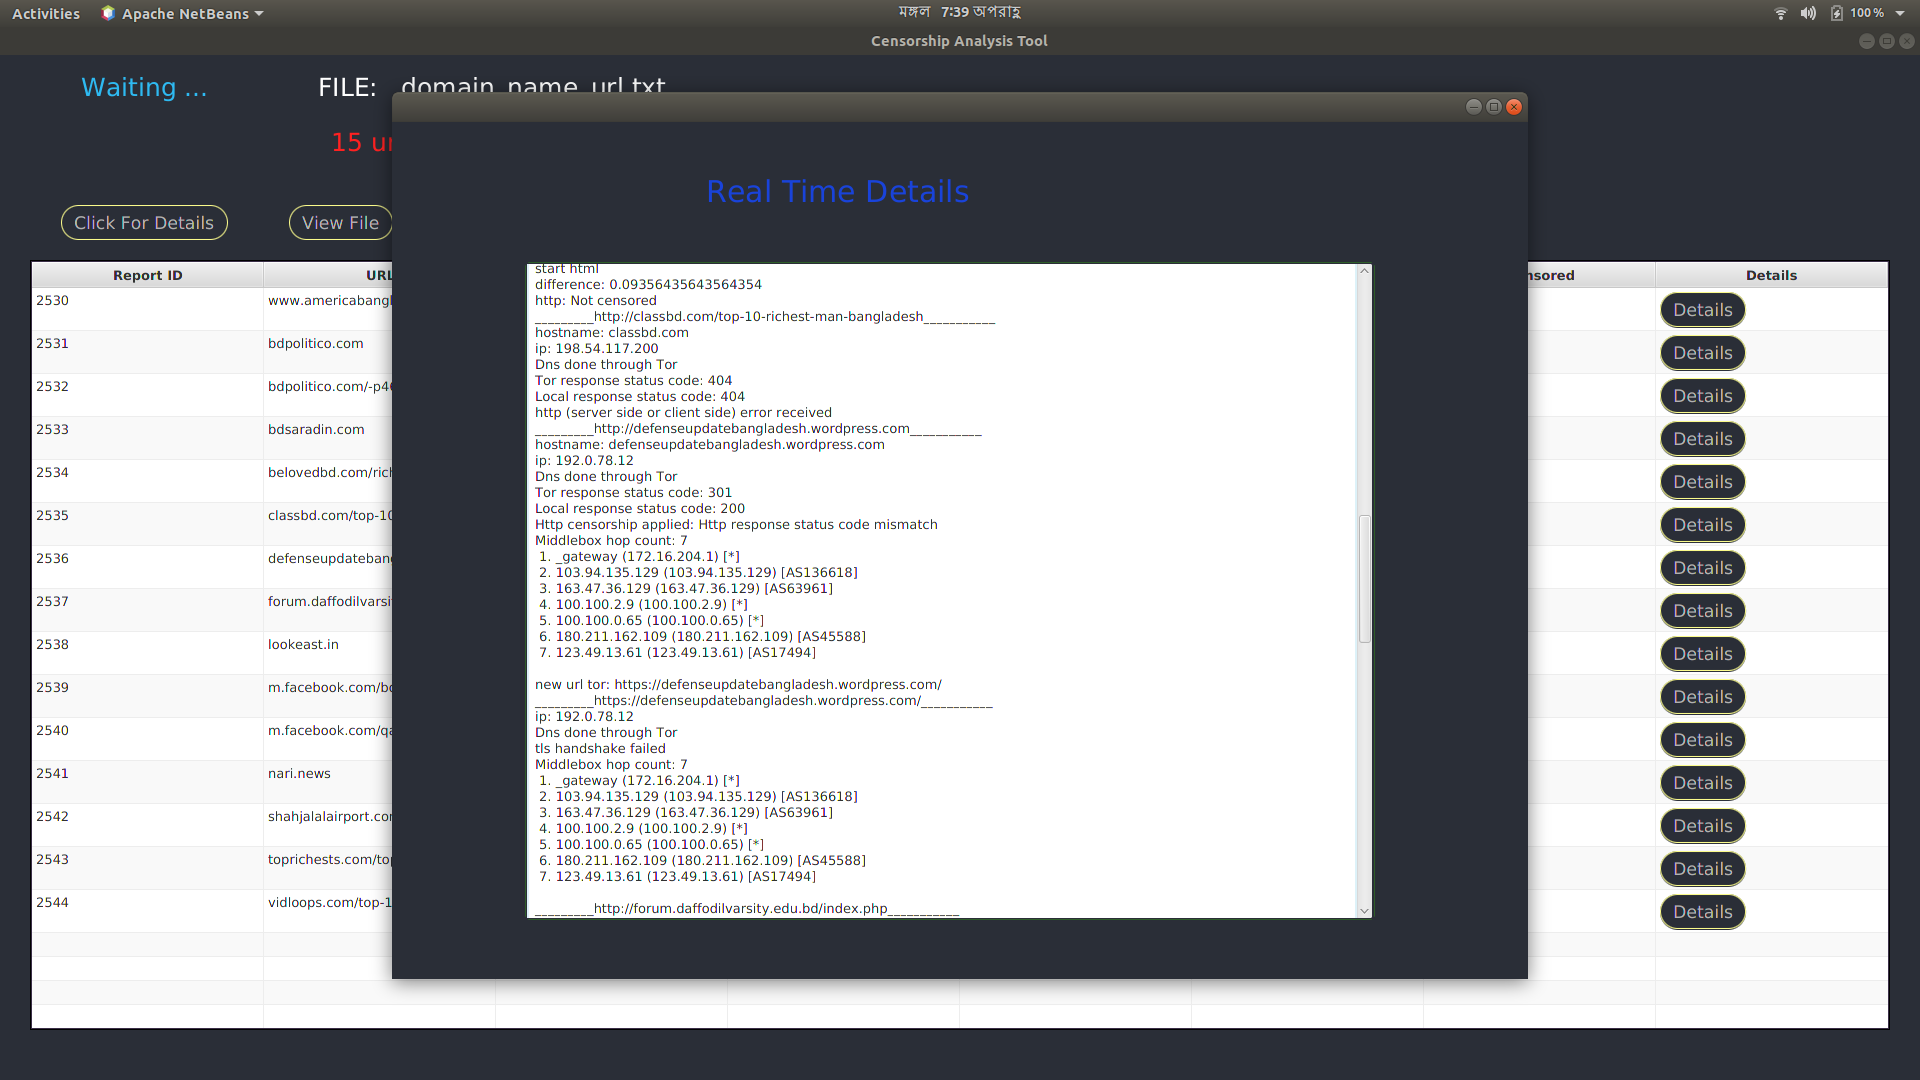
\includegraphics[width=\textwidth]{usersite/35realtimedetails.png}
    \caption{HTTP real time operations are going on}
    \label{fig:user35}
\end{figure}

\begin{figure}[h]
    \centering
    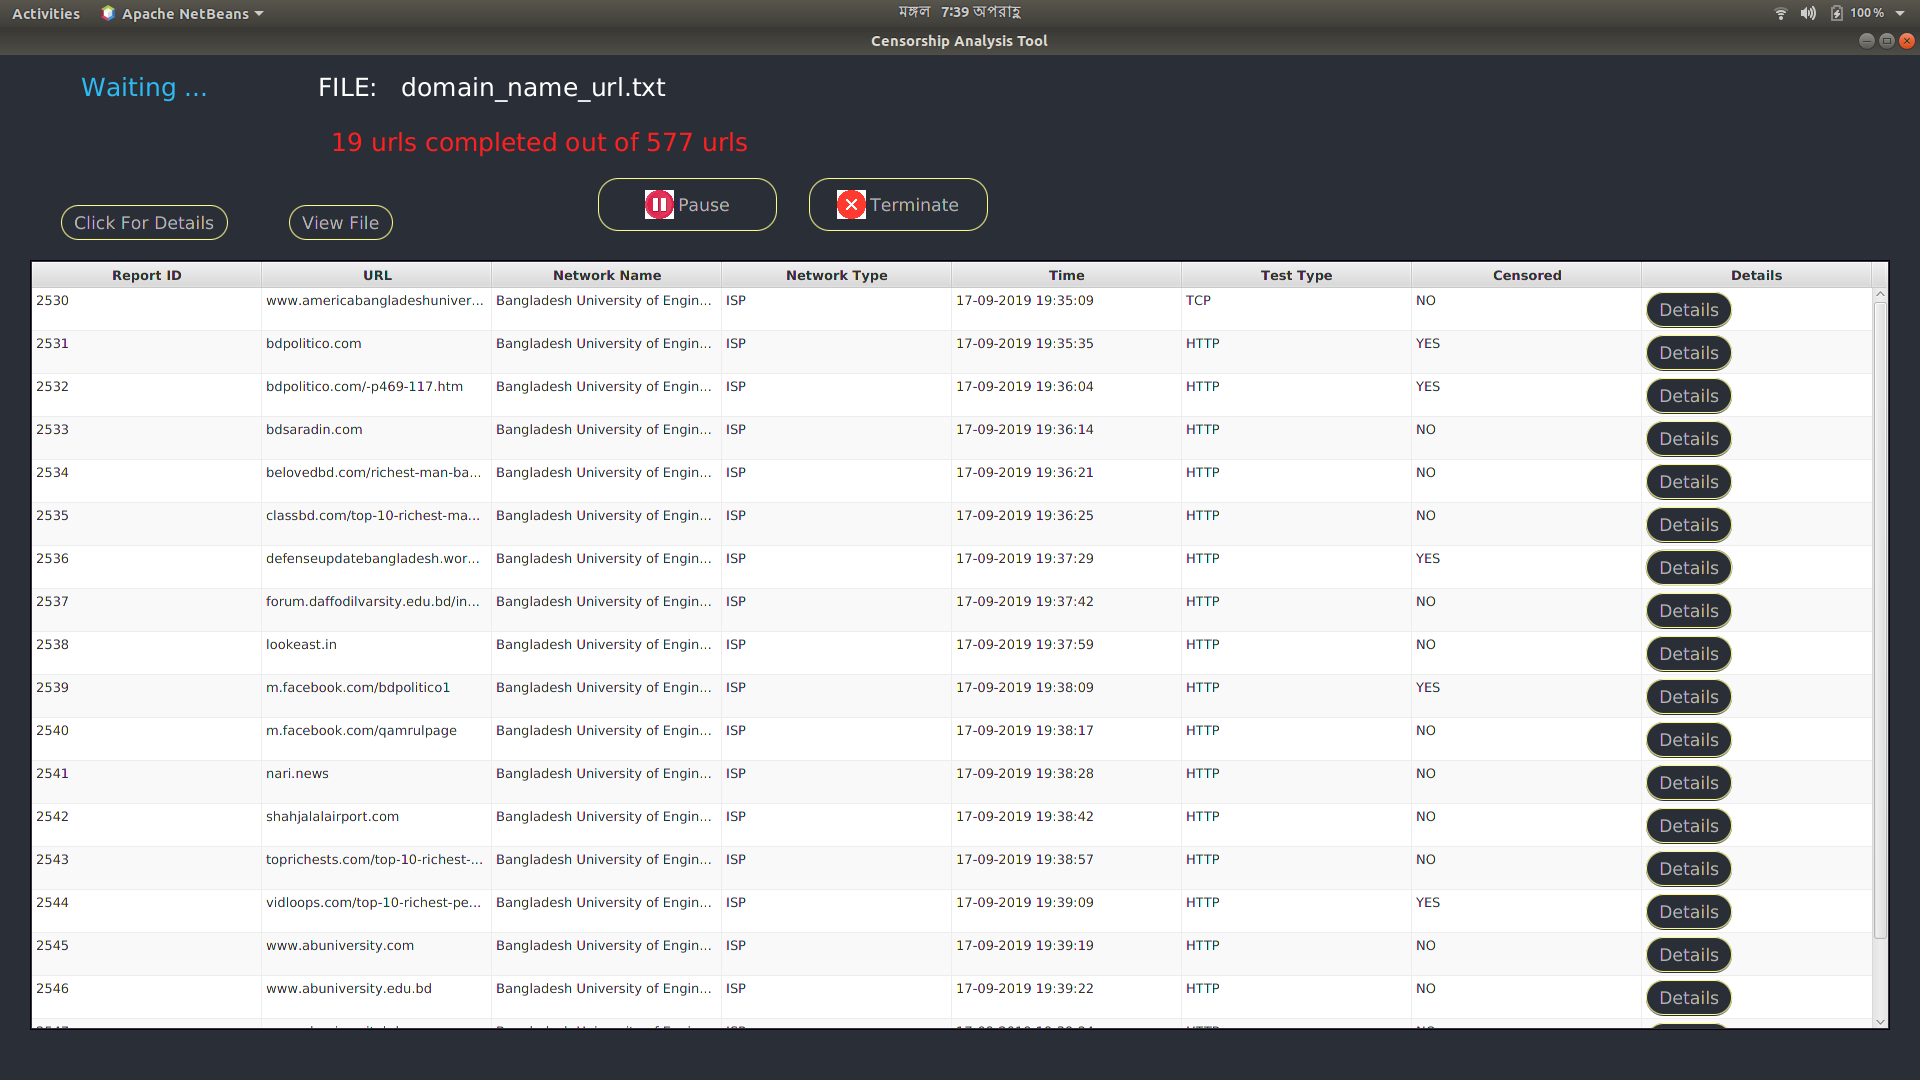
\includegraphics[width=\textwidth]{usersite/36completing.png}
    \caption{19 URLS completed out of 577}
    \label{fig:user36}
\end{figure}
